\NeedsTeXFormat{LaTeX2e}
\documentclass[a4paper,12pt,
headsepline,           % Linie zw. Kopfzeile und Text
oneside,               % einseitig
pointlessnumbers,      % keine Punkte nach den letzten Ziffern in Überschriften
bibtotoc,              % LV im IV
%DIV=15,               % Satzspiegel auf 15er Raster, schmalere Ränder   
BCOR15mm               % Bindekorrektur
%,draft
]{scrbook}
\KOMAoptions{DIV=last} % Neuberechnung Satzspiegel nach Laden von Paket helvet
\makeatletter
\newcommand\notsotiny{\@setfontsize\notsotiny{7.5}{8.5}}
\makeatother

\pagestyle{headings}
\usepackage{booktabs}
\usepackage{makecell}
\usepackage{multirow}
\usepackage{geometry}
\usepackage{adjustbox}
\usepackage{longtable}
\usepackage{caption}
\captionsetup{font=tiny}
\usepackage{anyfontsize}


% für Texte in deutscher Sprache
\usepackage[english]{babel}
\usepackage[utf8]{inputenc}
\usepackage[T1]{fontenc}
%\geometry{a4paper, margin=1in}
\geometry{a4paper, margin=1in}
\usepackage{flafter} % make sure figures do not appear before their text

\usepackage[scaled]{helvet}
\renewcommand{\familydefault}{\sfdefault} 

\usepackage{graphicx}

% Literaturverzeichnis mit BibLaTeX
% Include the natbib package
\usepackage[numbers]{natbib}

% The bibliography style
\bibliographystyle{apalike}

\usepackage[babel,english=quotes]{csquotes}
\usepackage[backend=bibtex8]{biblatex}
\usepackage[backend=biber]{biblatex}
\usepackage{placeins}
\usepackage{algorithm}
\usepackage{algpseudocode} 
\usepackage{bbm}



%%% --- The following two lines are what needs to be added --- %%%
\setcounter{biburllcpenalty}{7000}
\setcounter{biburlucpenalty}{8000}
\bibliography{bibliography}

% Alternative mit Paket-Option backend=biber und \addbibresource
% \usepackage[backend=biber]{biblatex}
% \addbibresource{bibliography.bib}

% Für Tabellen mit fester Gesamtbreite und variabler Spaltenbreite
\usepackage{tabularx} 
\usepackage{graphicx}
\usepackage{subcaption}
\usepackage{float}
% Besondere Schriftauszeichnungen
\usepackage{url}              % \url{http://...} in Schreibmaschinenschrift
\usepackage{color}            % zum Setzen farbigen Textes
\usepackage[nottoc]{tocbibind}
\usepackage{booktabs} % Für schönere Tabellenlinien
\usepackage{array}

\usepackage{amssymb, amsmath} % Pakete für Mathe-Umgebungen und -Symbole
\usepackage{todonotes}
\usepackage{setspace}         % Paket für div. Abstände, z.B. ZA
%\onehalfspacing              % nur dann, wenn gefordert; ist sehr groß!!
\setlength{\parindent}{0pt}   % kein linker Einzug der ersten Absatzzeile
\setlength{\parskip}{1.4ex plus 0.35ex minus 0.3ex} % Absatzabstand, leicht variabel

% Tiefe, bis zu der Überschriften in das Inhaltsverzeichnis kommen
\setcounter{tocdepth}{3}      % ist Standard

% Beispiele für Quellcode
\usepackage{listings}
\lstset{language=Python,
  showstringspaces=false,
  frame=single,
  numbers=left,
  basicstyle=\ttfamily,
  numberstyle=\tiny}

% hier Namen etc. einsetzen
\newcommand{\fullname}{Tanja Zast}
\newcommand{\email}{tanja.zast@uni-ulm.de}
\newcommand{\titel}{Exploratory Applications on Apple Watch Ultra Datasets in the Context of the \newline
6-Minute Walk Test}
\newcommand{\jahr}{2024}
\newcommand{\matnr}{935593}
\newcommand{\gutachterA}{Prof.\,Dr.\,Rüdiger Pryss}
\newcommand{\gutachterB}{Prof.\,Dr.\,Manfred Reichert}
\newcommand{\betreuer}{Dr. Michael Winter}

% hier die Fakultät auswählen
%\newcommand{\fakultaet}{---  Im Quellcode anpassen nicht vergessen! ---}
\newcommand{\fakultaet}{Engineering, \\ Computer Science \\ and Psychology}
%\newcommand{\fakultaet}{Mathematik und\\Wirtschafts-\\wissenschaften}
%\newcommand{\fakultaet}{Medizin}
%\newcommand{\fakultaet}{Naturwissenschaften}

% hier das Institut einsetzen
\newcommand{\institut}{Institute of Databases and Information Systems}

% Informationen, die LaTeX in die PDF-Datei schreibt
\pdfinfo{
  /Author (\fullname)
  /Title (\titel)
  /Producer     (pdfeTex 3.14159-1.30.6-2.2)
  /Keywords ()
}
\usepackage{longtable}
\usepackage{hyperref}
\usepackage{multirow}
\hypersetup{
pdftitle=\titel,
pdfauthor=\fullname,
pdfsubject={Diplomarbeit},
pdfproducer={pdfeTex 3.14159-1.30.6-2.2},
colorlinks=false,
pdfborder=0 0 0	% keine Box um die Links!
}

% Trennungsregeln
\hyphenation{Sil-ben-trenn-ung}

\begin{document}
\frontmatter

% Titelseite
\thispagestyle{empty}
\begin{addmargin*}[4mm]{-10mm}

\hfill

\includegraphics[height=1.8cm]{images/logo_uulm_sw.png}\\[1em]

{\footnotesize
%{\bfseries Universität Ulm} \textbar ~89069 Ulm \textbar ~Germany
\hspace*{115mm}\parbox[t]{35mm}{\bfseries Faculty of\\
\fakultaet\\
% TODO hier Institut anpassen
\mdseries \institut}\\[2cm]

\parbox{140mm}{\bfseries \LARGE \titel}\\[2.5em]
{\footnotesize Master Thesis at Ulm University}\\[3em]

{\footnotesize \bfseries Submitted by:}\\
{\footnotesize \fullname\\ \email}\\ \matnr\\[2em]
{\footnotesize \bfseries Reviewers:}\\                     
{\footnotesize \gutachterA\\ \gutachterB}\\[2em]
{\footnotesize \bfseries Supervisor:}\\ 
{\footnotesize \betreuer}\\\\
{\footnotesize \jahr}
}
\end{addmargin*}


% Impressum
\clearpage
\thispagestyle{empty}
{ \small
  \flushleft
  Version \today \\\vfill
  \copyright~\jahr~\fullname\\[0.5em]
% Wenn Sie Ihre Arbeit unter einer freien Lizenz bereitstellen möchten, können Sie die nächste Zeile in Ihren Code aufnehmen. Bitte beachten Sie, dass Sie hierfür an allen Inhalten, inklusive enthaltener Abbildungen, die notwendigen Rechte benötigen! Beim Veröffentlichungsexemplar Ihrer Dissertation achten Sie bitte darauf, dass der Lizenztext nicht den Angaben in den Metadaten der genutzten Publikationsplattform widerspricht. Nähere Information zu den Creative Commons Lizenzen erhalten Sie hier: https://creativecommons.org/licenses/
%This work is licensed under the Creative Commons Attribution 4.0 International (CC BY 4.0) License. To view a copy of this license, visit \href{https://creativecommons.org/licenses/by/4.0/}{https://creativecommons.org/licenses/by/4.0/} or send a letter to Creative Commons, 543 Howard Street, 5th Floor, San Francisco, California, 94105, USA. \\
  Composition: PDF-\LaTeXe
}

% ab hier Zeilenabstand etwas größer 
\setstretch{1.2}
\newenvironment{abstract}%
    {\cleardoublepage\thispagestyle{empty}\null\vfill\begin{center}%
    \bfseries Abstract\end{center}}%
    {\vfill\null}
        \begin{abstract}
        \footnotesize{This master thesis investigates the usability of data sets from the Apple Watch Ultra in the context of the 6-Minute Walk Test using machine learning techniques. The aim of the study is to evaluate the reliability and applicability of data from wearable technologies, focusing exclusively on the Apple Watch Ultra. By integrating additional health metrics such as body mass index, blood pressure and demographic variables, the predictive power of ML models in predicting health outcomes and detecting potential risks will be investigated.
        
        Key contributions include the application of various machine learning models, including supervised and unsupervised learning techniques, to analyze heart rate, energy expenditure and distance walked recorded during the 6-Minute Walk Test. The study highlights the importance of comprehensive data analysis and the potential of the Apple Watch Ultra. The results demonstrate the effectiveness of machine learning methods in improving the accuracy of health predictions and provide valuable insights into the strengths and limitations of using Apple Watch Ultra data for specific applications. 

        The complete code and all programmed models used in this study can be accessed in the GitHub repository ~\cite{githubMasterthesisjupyter_folderMain}.
        }
        \end{abstract}
        \clearpage
\newenvironment{acknowledgements}%
    {\cleardoublepage\thispagestyle{empty}\null\vfill\begin{center}%
    \bfseries Acknowledgements\end{center}}%
    {\vfill\null}
        \begin{acknowledgements}
        \footnotesize{Enormous gratitude is extended to all those who contributed to the success of this master thesis through their professional and personal support.

        Special thanks go to my supervisor Michael Winter, who provided the ideal conditions for this work. His knowledge and unwavering support at any time of day have been invaluable.

        I also extend my deep appreciation to Prof. Dr. Manfred Reichert and Prof. Dr. Rüdiger Pryss for their invaluable feedback and for serving as reviewers of this thesis. Their insights and suggestions have greatly enhanced the quality of this work.

        Additional thanks to Mathis Rost for his unwavering support, meticulous proofreading, and for challenging the methodology part of this work with critical questions.

        I am also grateful to Jonathan Wunden, Max Friemann, and especially Emma Osbourn for their constructive criticism and helpful feedback throughout this process.

        Finally, heartfelt thanks go to friends, family and Pepe for their constant encouragement, especially during challenging times when results were not as expected. Their support has been crucial in completing this journey.}
        \end{acknowledgements}
        \clearpage
\tableofcontents

\mainmatter
\chapter{Introduction}

In recent years, wearable technology has revolutionized health monitoring. Devices such as the Apple Watch, iPhone and Samsung smartphones play an important role in recording and analyzing health data. But they are also of great interest in the field of physical examinations ~\cite{healthtechmagazineLatestTrends}.

In addition to physical examinations, wearable technology also has a significant impact on the way athletes train and monitor their progress in sports and fitness. For example, the advanced sensors in these devices can track heart rate, oxygen saturation, sleep patterns and physical activity levels with high precision. This detailed monitoring allows athletes and fitness enthusiasts to gain insights into their performance, recovery and overall health ~\cite{doi:10.1177/1941738115616917}.

It was the integration of artificial intelligence (AI) into wearable technology, that has further enhanced its capabilities. AI algorithms can analyze the vast amounts of data collected by these devices to provide personalized feedback and recommendations. For example, AI can help predict potential injuries. This real-time analysis and feedback allows users to make informed decisions about their health routines ~\cite{s22186920}.

The combination of wearable technology and AI not only helps with personal health monitoring, but also opens up new possibilities for remote treatment. One example is the 6-Minute Walk Test (6MWT), which is often used to assess functional performance and predict cardiovascular and respiratory diseases. In this paper, the 6MWT is particularly emphasized as the University of Würzburg used this test for data collection with the Apple Watch Ultra. The data obtained from this test is directly incorporated into the study and is therefore an essential part of the methodology and analysis of the thesis. Patients can perform tests such as the 6MWT at home, and the data can be analyzed and shared with healthcare professionals in real time. This advance can be particularly beneficial in the treatment of chronic diseases, where continuous monitoring and timely interventions are crucial ~\cite{s22020581}.

This thesis will focus on investigating the efficiency of machine learning (ML) methods when using data collected exclusively from the Apple Watch Ultra, particularly in predicting health metrics. The key research questions guiding this study are: What data provided by the Apple Watch Ultra related to the 6MWT can be effectively utilized in ML models? Can we achieve reliable and accurate results with ML applications using only the data measured by the Apple Watch Ultra? Is the inclusion of non-Apple Watch Ultra data improving the performance and accuracy of ML models? By answering these questions, this research aims to identify the strengths and limitations of using data from wearable technologies for ML and ultimately optimize the integration of these technologies for improved health outcomes.

\section{Motivation}

The motivation behind this work is to investigate the accuracy of ML methods and clinical relevance of data from smartwatches such as the Apple Watch Ultra, particularly during the 6MWT. Many fitness enthusiasts already rely on data from these devices, but questions remain about their data reliability. Particularly in medical facilities, but also in clinical settings, this data reliability is fundamental ~\cite{b58999084d4b43b8bea456c509edf858}.

The aim of this thesis is to utilize the advanced sensors and data collection capabilities of the Apple Watch Ultra to train and test ML models. These models will predict health outcomes and identify potential health risks based on 6MWT data. The main goal is to evaluate the accuracy of the Apple Watch Ultra data and determine its utility for clinical applications.

This work builds on a detailed protocol and utilizes a dataset collected during a study involving the 6MWT. The focus is on integrating data from the Apple Watch Ultra with ML techniques to enhance health monitoring. By incorporating additional physiological and demographic variables such as blood pressure, sex and age, the predictive power and model performance will be improved.

This research also aims to close the gap in the clinical applicability of data from wearable technologies. It will collect and process data from the Apple Watch Ultra during the 6MWT to ensure it is ready for ML analysis. Both supervised and unsupervised ML models will be developed to analyze heart rates, running distances and other indicators during the 6MWT.

\section{Problem Statement and Research Question}

The aim of this research is to verify the accuracy and functionality of the Apple Watch Ultra during the 6MWT. By using ML, we hope to improve health predictions and better assess potential risks. The study addresses the research question of what data the Apple Watch Ultra provides and how this data can be used effectively in the field of supervised and unsupervised learning.

\section{Structure}

The paper is structured to systematically address the key challenges. The introductory chapter outlines the aims of the study, the problem statement and the general structure.

The second chapter contains the medical and technical background to which reference is made in the remainder of the work.

Chapter three, 'Related Work' [~\ref{cha:relatedwork}] provides an overview of the existing literature on ML in health monitoring, focusing on wearable technology and the 6MWT.

Chapter four, 'Methodology' [~\ref{cha:methods}] explains the data collection, pre-processing steps and the ML models used for analysis.

Chapters five and six, 'Example Dataset' [~\ref{cha:exampleDataset}] and 'Analyzing the Study Dataset' [~\ref{cha:studyDataSet}] discuss the structure of the collected dataset and present the initial results of the exploratory data analysis. This leads on to chapter seven, 'Implementation and Results' [~\ref{cha:results}], which covers the practical implementation of various ML models, such as linear regression, random forests and deep learning techniques. This chapter also presents the results of the model evaluations, including performance metrics and comparisons with existing methods.

Chapter eight, 'Improving Model Performance with additional Health Data' [~\ref{cha:resultsaddFeatures}] deals with specific improvements and experiments. It includes sections on distance measurement accuracy and analyzing blood pressure data, adding more measures to the dataset. Each section addresses different ways to improve data analysis and prediction accuracy.

Finally, chapter nine, 'Discussion and Further Work' [~\ref{cha:discussion}], delves into the implications of the findings, addresses the limitations of the study, and proposes suggestions for future research. Additionally, it outlines preliminary experiments and approaches for further work, including the use of a larger dataset to enhance the robustness and generalizability of the results.
\chapter{Medical and Technological Background}
\label{cha:background}

This chapter contains all the medical and technical information that can help in the further course of the work. We will cover key concepts related to heart rate, the 6MWT, body mass index, heart rate measurement with the Apple Watch and a comparison of various technical devices.

\section{Heart Rate}
Heart rate (HR) refers to the number of heartbeats per minute. When the body is at rest, this rate is called the resting heart rate. The resting heart rate is an important measure for assessing heart function and varies between individuals. It is a key indicator of cardiovascular health and physical fitness, with a normal resting heart rate ranging from 60 to 100 beats per minute ~\cite{heart}.

Various factors can affect heart rate, including age, sex, fitness level, medications, and underlying health conditions.

Even resting heart rate can differ among individuals. Women often have a slightly higher heart rate than men. Research by ~\textcite{HeartRate_study} shows that women's resting heart rates are typically 8-10 beats per minute higher than men's. For adult men, the average resting heart rate ranges from 70 to 72 beats per minute, while for adult women, it generally ranges from 78 to 82 beats per minute.

Women generally have smaller hearts than men, requiring a faster beat to circulate the same amount of blood. Additionally, studies like ~\textcite{Ryan1994GenderAA} suggest that women's heart pacemakers have a unique intrinsic rhythm, resulting in naturally faster heartbeats.

\section{6-Minute Walk Test}

The 6MWT is a practical and widely used measure of functional exercise capacity, as detailed by ~\textcite{6MWT}. 
It measures how far a patient can walk in six minutes, reflecting their ability to perform daily activities. This test provides an overall assessment of a patient’s respiratory, cardiovascular, neuromuscular, and cognitive functions. Unlike tests that measure maximal exercise capacity, the 6MWT evaluates a patient’s functional level during everyday activities ~\cite{6MWT}.

The American Thoracic Society's guidelines highlight the test's safety, ease of administration, and its better reflection of daily activities compared to other walk tests. 

The primary measurement is the 6-Minute Walk Distance (6MWD), but it also provides data on blood oxygen saturation and the patient's perception of exertion ~\cite{6MWT}.

The work by ~\textcite{6MW-ML} emphasizes the importance of accurately assessing dynamic balance ability in the elderly, critical for fall risk assessment and overall health monitoring. This research uses ML models to predict the age of elderly individuals based on their performance in the 6MWT, utilizing data from an Inertial Measurement Unit. The study collected data, extracted features related to movement and balance, and trained ML models like Random Forest (RF) and Gradient Boosting Machine (GBM) to predict the participants' ages. The combined features from both  Instrumented Timed Up and Go and 6MWT yielded the best performance, indicating a strong correlation between the Digital Biomarker Analysis and the chronological age. The study concludes that ML-enhanced 6MWT could be effective tools for Digital Biomarker Analysis assessment.

~\textcite{6MWtech} provide a systematic review of various studies using sensor technologies to monitor the 6MWT. The review covers studies from 2016 to 2021 and includes diseases like multiple sclerosis, pulmonary diseases, heart diseases, brain injuries, bone diseases, and kidney diseases. Most studies used motion and inertial sensors in devices, with some employing Diffusion Tensor Imaging and GPS technologies. The review highlights the importance of medical collaboration and the potential of sensor technologies for remote and continuous monitoring of 6MWT performance, enhancing patient care and disease management.

The paper by ~\textcite{ROMERO2022107020} outlines a methodology to predict 6MWT outcomes in Chronic Obstructive Pulmonary Disease patients using clinical and cardiopulmonary parameters without performing the test physically. The study collects data such as anthropometric data, spirometry parameters, and physiological data. It uses analytical techniques to extract heart rate variability indices from Electrocardiogram (ECG) data, incorporating these into a predictive model. The model employs lasso regularization for feature selection and ordinary least squares regression for final formation. Individual models estimate 6MWT outcomes like total distance walked, maximum heart rate achieved, and heart rate recovery, and a Bayesian network couples these models for simultaneous estimation. The models show moderate to strong correlations between predicted and actual measures, suggesting potential for remote patient monitoring and personalized care in Chronic Obstructive Pulmonary Disease patients where physical performance tests are not feasible.

\section{Body Mass Index}

The body mass index (BMI) is a widely used and straightforward index that calculates the ratio of weight to height to categorize individuals into different weight statuses. This method offers a quick way to assess potential health risks associated with body fat.

The World Health Organization (WHO) provides a standardized table and formula for BMI categorization, which has been instrumental in this research ~\cite{whoHealthyLifestyle}. The table below summarizes the WHO BMI categories:

\begin{table}[ht]
    \centering
\begin{tabular}{|l|r|}
\hline
\textbf{BMI} &  \textbf{nutritional status}  \\ \hline
< 18.5            &   underweight\\ \hline
18.4 - 24.9       &   normal weight \\ \hline
25.0 - 29.9       &   pre-obesity \\ \hline
30.0 – 34.9       &   obesity class I \\ \hline
35.0 – 39.9       &   obesity class II \\ \hline
> 39.9            &   obesity class III \\ \hline
\end{tabular}
\caption{WHO BMI categorization}
\label{table:BMI}
\end{table}

According to WHO guidelines, BMI categories help in identifying individuals at risk for health issues such as cardiovascular diseases, diabetes, and other conditions related to overweight and obesity ~\cite{whoHealthyLifestyle}. In this work, the guidelines of table ~\ref{table:BMI} are used to analyze the health risk of the participants and to add an additional health factor that can be quickly evaluated.

The formula for calculating BMI is the following:

\begin{equation}
    BMI = \frac{\text{weight (kg)}}{\text{height (m)}^2}
\end{equation}

This formula divides a person's weight in kilograms by the square of their height in meters, resulting in a value that can be used to determine their BMI category. By applying this formula, we can categorize individuals and assess their potential health risks based on the standardized BMI ranges provided by the WHO.

\section{Heart Rate Measurement with Apple Watch}

The Apple Watch uses advanced technology to measure heart rate. This section explains how the Apple Watch measures heart rate and the functionalities of these measurements ~\cite{AppleSupport120277}.

The main technology used in the Apple Watch for heart rate measurement is photoplethysmography. This technique works on the principle that blood reflects red light and absorbs green light. In detail it uses green LED lights and light-sensitive photodiodes to detect blood flow in the wrist. The green LEDs flash hundreds of times per second, allowing the Apple Watch to measure heart rate by observing changes in light absorption caused by blood flow. The optical heart sensor can measure heart rates between 30 to 210 beats per minute, adjusting the LED brightness and sampling rate for accuracy, even with low signal levels.

\FloatBarrier
\begin{figure}[h!]
\centering
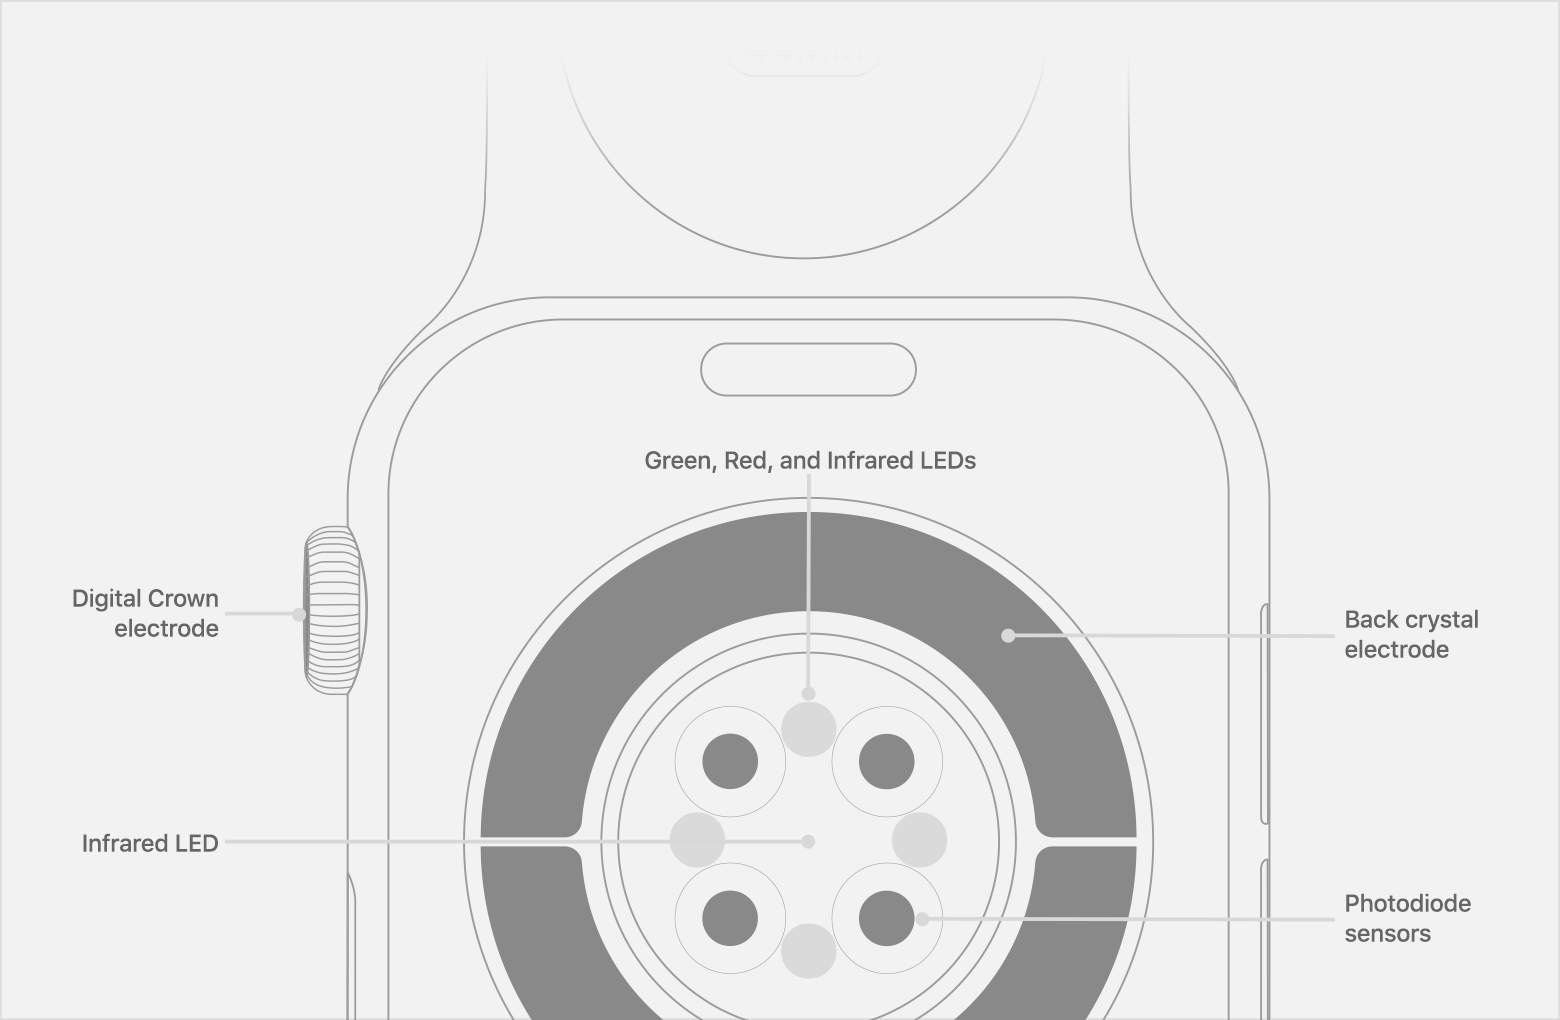
\includegraphics[width=0.85\textwidth]{Master Thesis/Plots/apple-watch-series6-measure-sensors.png}
\caption{Diagram of the Apple Watch sensors}
\label{fig:applewatch}
\end{figure}
\FloatBarrier

Figure ~\ref{fig:applewatch} shows the back of an Apple Watch, highlighting its sensors and components. It includes the 'Digital Crown Electrode' on the side and the 'Back Crystal Electrode' underneath for taking ECG readings. The Infrared LED, used for background heart rate measurement and notifications, is located around the sensor area. The central optical heart sensor, with green, red, and infrared LEDs, is essential for detecting blood flow and measuring heart rate. Photodiode sensors nearby detect reflected light from the skin to calculate heart rate. This setup enables the Apple Watch's comprehensive health monitoring features.

Besides using green LED lights, the optical heart sensor can also use infrared light for heart rate measurement. This mode is generally used for background heart rate monitoring and notifications. During active sessions such as workouts and Breathe sessions, the green LEDs are used to calculate metrics like walking average and heart rate variability ~\cite{AppleSupport120277}.

Starting with the Apple Watch Series 4 and including all models of the Apple Watch Ultra, the device features built-in electrodes in the 'Digital Crown' and the back of the watch. These electrodes measure electrical signals across the heart. When used with the Heart Rate app or the ECG app, placing a finger on the Digital Crown creates a closed circuit between the heart and both arms, capturing electrical impulses across the chest.

To use the electrical heart sensor for heart rate measurement, open the 'Heart Rate' app and place a finger on the 'Digital Crown'. This method provides a faster and more accurate reading, capturing data every second instead of every five seconds. Recorded data in the Health app will show 'ECG' in the 'Heart Rate' context ~\cite{AppleSupport120277}.

\section{Comparison to other Technical Devices}

The table below shows the performance of various fitness trackers in terms of distance and step count accuracy, as well as their battery life ~\cite{nytimesBestFitness}:

\FloatBarrier
\begin{table}[h!]
\centering
\begin{tabular}{|>{\raggedright}p{4cm}|>{\raggedright}p{2.5cm}|>{\raggedright}p{2cm}|>{\raggedright\arraybackslash}p{2cm}|}
\hline
\textbf{Product} & \textbf{Distance accuracy (miles)$^1$} & \textbf{Step count accuracy (\%)$^2$} & \textbf{Remaining battery life (48h)} \\
\hline
Amazfit Band 7 & $\downarrow$ 0.09 & $\uparrow$ 2 & 90\% \\
\hline
Apple Watch SE & $\downarrow$ 0.04 & $\uparrow$ 0.50 & 9\% (after 18 hours of testing) \\
\hline
Fitbit Charge 5 & $\downarrow$ 0.01 & $\uparrow$ 2 & 70\% \\
\hline
iPhone 15 & n/a & n/a & 0\% (after 20 hours of testing)\\
\hline
iPhone 13 mini & n/a & n/a & 0\% (after 17 hours of testing)\\
\hline
\multicolumn{4}{l}{\footnotesize{$^1$ According to 1-mile treadmill test (but without iPhone 13 mini and 15).
$^2$ \% error}}
\end{tabular}
\caption{Fitness tracker performance}
\end{table}
\FloatBarrier

The Fitbit Charge 5 stands out for its high accuracy in both distance and step counts, and a decent remaining battery life. The Apple Watch SE also performs well in terms of tracking accuracy but has a significantly shorter battery life compared to the other devices.

The data for the iPhone 13 mini and iPhone 15, while included for comparison, are marked as 'n/a'. This is because the rest of the table uses general values for continuous fitness tracking, and specific data for these values is not available. Although it is technically possible to obtain this information from our existing data, doing so would result in inconsistent references across the table.

In this study, we focus exclusively on the Apple Watch Ultra, emphasizing the new generation's capabilities in health monitoring and prediction through the use of ML, what we will define more detailed later. The aim of this study is to evaluate the accuracy and reliability of the Apple Watch's measurements and to explore both its potential and limitations.
\chapter{Related Work}
\label{cha:relatedwork}

This chapter presents important work in the areas of machine learning, 6MWT and the use of ML with wearable devices. A lot of research is being done in these areas and there are many exciting developments and discoveries. ML is a rapidly growing field and 6MWT has also been studied a lot for its medical and fitness applications. The combination of machine learning with wearable devices, especially the Apple Watch Ultra, particularly for the 6MWT, is a new and promising area of research.

We will focus on how ML can be applied to the 6MWT using the Apple Watch Ultra.  A more detailed related work part is already shown in chapter ~\ref{cha:background}.

This chapter presents a selection of papers that have contributed to these topics. By looking at the methods used in previous research, we will provide a basis for understanding the current state of knowledge. We will also explain how our work differs and what new contributions we aim to make.

\section{Classification and Regression Tasks for Apple Watch Data}

In ML, classification and regression are fundamental tasks within supervised learning. Supervised learning involves training a model on labeled data, where the model learns from input-output pairs. Classification predicts discrete, categorical labels, such as determining if an individual is a subject or a patient, while regression predicts continuous values, such as estimating the age based on heart rate data. These methods can be interrelated, where regression models are used for classification by converting categories into numerical values and applying thresholds to determine the classes ~\cite{bishop2006pattern}.

Previous studies have utilized various ML models to predict health outcomes from wearable sensor data. These models include Support Vector Machines (SVM), random forests, and neural networks. For example, ~\textcite{Bailey} used SVMs to classify cardiovascular risk based on heart rate variability data. An SVM is a supervised learning model that classifies data by finding the optimal hyperplane that separates different classes in a high-dimensional space.

The study by ~\textcite{Bailey} aims to develop and evaluate the accuracy of a method using the inertial measurement unit of a consumer-grade smartwatch to predict gait outcomes using regression-based ML techniques. An inertial measurement unit measures and reports a body's specific force, angular rate, and sometimes the surrounding magnetic field, using a combination of accelerometers, gyroscopes, and magnetometers. Regression models are particularly effective for predicting continuous values such as stride time, stride length, stride width, and walking speed.

The work of ~\textcite{Bailey} additionally uses extreme gradient boosting, another regression techniques. Extreme gradient boosting is a ML algorithm that handles complex, non-linear relationships well and is robust against overfitting, which occurs when a model learns the training data too well, including its noise and outliers, leading to poor generalization to new data ~\cite{Stojancic}. Similarly, the kernel SVM captures non-linear relationships in data effectively, making it useful for predicting complex patterns.

Compared to ~\textcite{Bailey} work, our study extends the research to different populations, from younger adults to older adults, to further refine the models. Additionally, the study explores the real-world application of the smartwatch-based model in the context of the 6MWT. This investigation assesses the model's effectiveness under varying environmental conditions, providing a broader understanding of its applicability and reliability in diverse scenarios.

\section{Pain Level Prediction with ML}

The work of ~\textcite{Stojancic} explores the potential of using the Apple Watch to predict pain levels in individuals with sickle cell disease during vaso-occlusive crises in a day hospital setting. This study develops and evaluates specific ML algorithms for this purpose, including multinomial logistic regression, gradient boosting, and random forest.

Multinomial logistic regression is chosen for its simplicity and effectiveness in handling multi-class classification problems. It extends logistic regression to scenarios where the dependent variable has more than two categories, making it suitable for predicting various pain levels.

Gradient boosting is an ensemble learning technique that builds models sequentially, with each new model correcting errors made by the previous ones. It is particularly powerful for handling complex, non-linear relationships in data.

Random forest, another ensemble learning method, is used primarily for its robustness and ability to manage high-dimensional data effectively. It constructs multiple decision trees during training and merges them to improve predictive performance and control overfitting.

The evaluation metrics employed in the study of ~\textcite{Stojancic} include accuracy, f1-score and root-mean-square error. Accuracy measures the proportion of correct predictions, the f1-score balances precision and recall, providing a single metric that considers both false positives and false negatives, and RMSE assesses the model's prediction error by calculating the square root of the average squared differences between predicted and actual values.

In our work, the focus is on increasing the sample size while minimizing the data measuring process due to the 6MWT interval for each subject. This approach aims to investigate whether it is possible to avoid class imbalance (where some classes have significantly more samples than others) while simultaneously improving model accuracy. Addressing class imbalance is crucial because it can lead to biased models that perform poorly on underrepresented classes. By expanding the dataset and optimizing the data collection process, this thesis seeks to enhance the reliability and precision of the predictive models while using similar metrics to the work of ~\textcite{Stojancic}.

\section{Deep Learning for Sleep Stage Classification}

The wok of \textcite{9754876} aims to develop a practical deep learning model for classifying sleep stages into four categories: wake, Rapid Eye Movement (REM), N1/N2 (light sleep stages), and N3 (deep sleep stage), using heart rate and acceleration data from consumer wearable devices.

The research of ~\textcite{9754876} uses a Gated Recurrent Unit (GRU)-based deep neural network model. GRUs are a type of recurrent neural network architecture specifically designed to capture temporal dependencies in sequential data. This characteristic is crucial for classification tasks where the temporal order of data points significantly impacts the outcome.

The model architecture comprises three bidirectional GRU layers. Bidirectional GRUs process the input data in both forward and backward directions, which allows the model to consider the entire sequence of data from both past and future contexts. This bidirectional approach enhances the model's ability to learn temporal dependencies more effectively, thereby improving classification accuracy.

To ensure a robust evaluation of the model's performance, our work employs a leave-one-subject-out validation and cross validation strategy. In the leave-one-subject-out validation method, the data from each subject is used exactly once for testing, while the data from all other subjects is used for training. This approach helps mitigate the risk of overfitting. By validating the model in this manner, we can ensure that the performance metrics reflect the model's ability to generalize across different subjects.

\newpage
This chapter has summarized some key papers and their main findings, describing the methods used and the contributions to the field of wearable device sensor data analysis. 

Our aim in this work is to demonstrate the significance and novelty of our approach, which combines the 6MWT with the advanced features of the Apple Watch Ultra and powerful machine learning techniques.
\chapter{Methodology}
\label{cha:methods}
In this chapter, we define all the methods and metrics that will be used in the later parts of this thesis. Our goal is to examine a diverse range of techniques to determine what works well and what does not, providing a comprehensive evaluation.

We will explore several prominent classification and regression techniques, including SVM, artificial neural networks, decision trees, and clustering. 

\section{Machine Learning}

In the context of ML, we start with a dataset \( X \) comprising various input-output pairs \((x, y)\). We hypothesize that there exists an underlying function \( f \) which accurately maps any input \( x \) to its corresponding output \( y \). Mathematically, this relationship is expressed as \( f(x) = y \). While the exact form of \( f \) is unknown, we attempt to approximate it with a function \( \hat{f} \). This approximation \( \hat{f} \) is then used to predict outputs \( \hat{y} \) for new inputs \( \hat{x} \).

To assess the performance of our approximation \( \hat{f} \), we employ a loss function \( L(y, \hat{y}) \), which quantifies the discrepancy between the true output \( y \) and the predicted output \( \hat{y} \) ~\cite{murphy2013machine}. The primary objective during the training phase of a machine learning model is to minimize this loss function over the training data, thereby improving the accuracy of our predictions.

The ultimate goal is to ensure that our model makes accurate predictions for new, unseen inputs ~\cite{murphy2013machine}. ML methodologies are broadly classified into two main categories.

\section{Supervised Learning}
The first is called predictive or supervised learning. Here, the goal is to figure out how to map inputs $x$ to outputs $y$, using examples where we already know the answers. We call these examples the training set $D$, and we label it as 
$D = \{(x_i, y_i)\}_{i=1}^N$,
where $N$ is how many data points we have.

In the simplest form, each input 
$x_i$ is a list of numbers, like someone's height and weight. We call these numbers features or attributes. But $x_i$ could be something more complex, like a picture or a sentence. The output 
$y_i$ could be something simple like a category, such as 'male' or 'female', or it could be a number, like for example someone's income level. When $y_i$ is a category, we call the problem classification. When $y_i$ is a number, it's called regression. There is also a special kind called ordinal regression, where the categories have a natural order, like grades from A to F ~\cite{murphy2013machine}.

\section{Classification}

When we have two classes, we usually have \( y \in \{0, 1\} \). This is called binary classification. If we have more than two classes, say \( C \) $\in \mathbb{N}$ classes, then \( y \in \{1, \ldots, C\} \), which is known as multiclass classification ~\cite{murphy2013machine}.

Sometimes, things can belong to more than one class at the same time. For example, someone can be both tall and strong. We call this multi-label classification. Mostly, we focus on predicting one class out of many, which is the multiclass classification ~\cite{murphy2013machine}.

In simple words, classification is about guessing which group, or class, something belongs to, so mathematically
\begin{equation}
    \hat{f}(x) = \underset{y \in Y} \arg \max p(y|x)
\end{equation}
Where $p(y|x)$ represents the probability distribution of the output $y$ given the input $x$ ~\cite{murphy2013machine}.

\subsection{Support Vector Machine}

SVMs are used to classify new given data by finding a hyperplane which separates the training set into different classes.\\ 
In the simple case of a SVM we only have two labels i.e. $Y \in \{0,1 \}^N$ and the space for our training data is given by $[X , Y] \in \mathbb{R}^d \times \{0,1 \}$, where $X$ is our training dataset and $Y$ the target space. The goal of the SVM is now to find a vector $w \in \mathbb{R}^d$ and a offset $b \in\mathbb{R}^d $ s.t. 
\begin{equation}
    \mathrm{sign}(w^T x_i +b) = y_i \qquad i \in \{1, \dots, d\}
\end{equation}
Therefore $w^T x + b = 0$ describes a hyperplane in $\mathbb{R}^d$. \\
In addition we want the hyperplane as far away as possible of both classes of the data.

More precise we want,
\begin{equation}
    (w,b) = \underset{(w,b)}{\mathrm{argmax}} \left (  \min_{(x,y)} \frac{w^T x + b}{ \lVert w \rVert} y \right )
\end{equation}

To optimize this is not easy at all,
therefore we define our minimum distance as $\kappa$. Which means that
\begin{equation}
    \kappa \leq (w^T x + b)y \text{ } \forall x \in X  \iff 1 \leq \left(\frac{w^T x}{\kappa} + \frac{b}{\kappa}\right)y \text{ } \forall x \in X 
\end{equation}
Therefore it is sufficient to optimize $\mathrm{argmax}_w \frac{1}{\lVert w \rVert}$ with the constraint $ 1 \leq (w^T x + b)y$. This can be optimized with help of Lagrange multipliers and gradient descent ~\cite{10.1023/A:1009715923555}. For technical reasons we optimize an equivalent problem, which is given by, 
\begin{equation}
    \underset{(w,b)}{\mathrm{argmin}} \frac{1}{2} \lVert w \rVert^2 \text{ with } 1 \leq (w^T x + b)y \text{ } \forall x \in X 
\end{equation}

Using the Lagrange multipliers method we obtain a linear combination with gives us the best possible hyperplane ~\cite{10.1023/A:1009715923555}. This can be expressed by, 
\begin{equation}
    w^T z + b = \sum_{(x,y)}  y \alpha_x  x^T z +b
\label{eq:SVM}    
\end{equation}
Where $z$ is a new data point and the $\alpha_x$ are the Lagrange multipliers. Note that our hyperplane is only depending on our training data. \\


\FloatBarrier
\begin{figure}[h!]
    \centering
    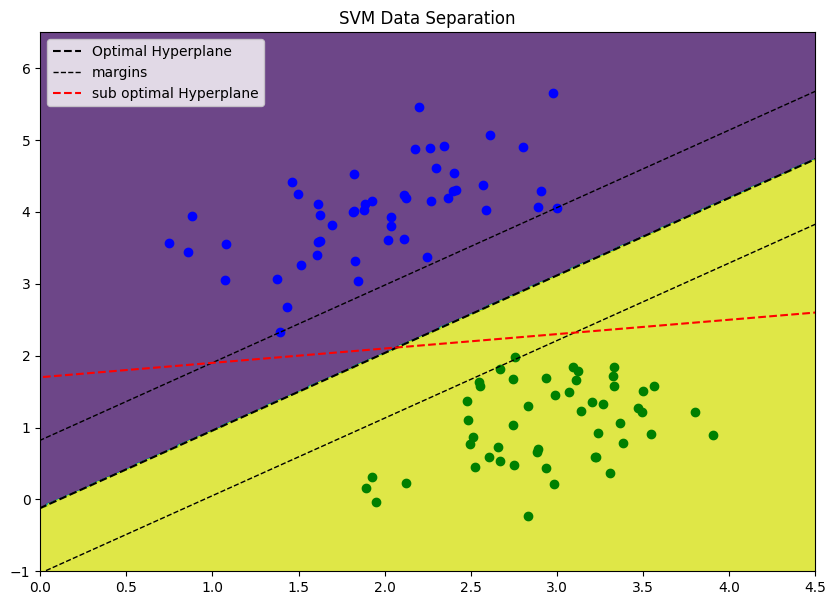
\includegraphics[width=0.7\textwidth]{Master Thesis/Plots/SVM.png}
    \caption{SVM linear dividing the space in to two regions to classify new data. The black line is the best possible line resulting out of a SVM.}
    \label{fig:SVM1}
\end{figure}
\FloatBarrier

Figure ~\ref{fig:SVM1} is an example of how SVM could look like in a visual case.

What is the approach if we have more than two classes? The solution for this problem is to use multiple SVMs, which then in combination can distinguish a single class. 
There are two common approaches: 'one-against-all' and 'one-against-one' ~\cite{PMID:18244442}.
In the one-against-all approach we need $m$ classifier for $m$ classes. The $i$-th classifier separates the $i$-th class from the remaining other $m-1$ classes. \\
The one-against-one approach is to use a classifier to linear separate all pairs of classes. This would need $\frac{m(m-1)}{2}$ classifier and is therefore computational more costly.

\subsection{Ensemble Learning}

In case of a classification task we can train multiple computational efficient, non deterministic models and make a majority vote for the label of a data point. Let $h_1, h_2, \cdots , h_t$ be such classifiers. With $h_{i \in \{1, \dots, t\}}: X \rightarrow Y$, where $X$ is our training dataset and $Y$ is our target space, we can express the majority vote $V(x)$ as 
\begin{equation}
    V(x) = \max_{y \in Y} (h_1(x), h_2(x) , \dots , h_t(x) )
\end{equation}

This diversity of the weak classifiers can lead to astonishing results ~\cite{book}. Examples for weak classifiers are RF and AdaBoost which are both really popular in practice ~\cite{book}.\\
To illustrate why Ensemble Learning can produce excellent results, consider the following example. 
\subsubsection{Wisdom of the Crowd}
Let $Y = \{0,1\}$, let $x_i \in X$ $\subset \mathbb{R}$ be a data point with label $y_i$. Let $\{h_1, \dots , h_t \} = \mathcal{H}$ be the set of classifiers. We assume that,
\begin{equation}
    P(h(x) = y) > \frac{1}{2} \text{ } \forall h \in \mathcal{H}
\label{eq:crowd}    
\end{equation}
Which means that a classifier will be correct more than half of the time.
We then see with Hoeffdings inequality ~\cite{book}, which is given by:
let $X_1, \dots, X_n $ be i.i.d. and there exist $a,b \in \mathbb{R}$ such that $a< X_i <b$, then 
\begin{equation}
    P \left[ \lvert \sum_{i=1}^n (X_i - \mathbb{E}[X_i])\rvert > \epsilon  \right] < 2 \exp \left ( - \frac{2n\epsilon^2}{(b-a)^2} \right )
\label{eq:Hoeffding}    
\end{equation}
that for large enough $t$ the majority vote will be most likely correct. Therefore consider the random variable $h_i$ with 
\begin{equation}
    h_i = 
    \begin{cases}
    1,& \text{if } h_i(x) = y\\
    0,              & \text{otherwise}
\end{cases}
\end{equation}
Since equation \eqref{eq:crowd} holds, we know there exists a $\delta > 0$ with 
$P(h_i) = \frac{1}{2} + \delta = \mathbb{E}[h_i]$. We now want to know what the probability is that the majority vote makes the correct decision i.e. $P\left [\sum_i^t h_i > \frac{t}{2} \right ]$. Taking the opposite event 
\begin{equation*}
    P \left [ \sum_i^t h_i \leq \frac{t}{2} \right] = P \left [ \frac{1}{t} \sum_i^t h_i - \frac{1}{t} \leq 0 \right] \leq P \left [ \lvert \frac{1}{t} \sum_i^t h_i - (\frac{1}{2} + \delta ) \rvert \leq \delta \right]
\end{equation*}

And with Hoeffding it now follows that,
\begin{equation*}
    P \left [ \sum_i^t h_i \leq \frac{t}{2} \right] \leq 2\exp \left ( -2t \delta^2 \right) \xrightarrow{t \rightarrow \inf} 0
\end{equation*}

This shows us, that under the described condition the probability that the majority vote is wrong goes to zero for a large amount of classifiers. However we assumed that our voters are independent, which is usually not the case. It still gives a good justification why Ensemble Learning can be strong. 

\subsection{Random Forest}

Kernel methods can provide a powerful way to create non-linear models for regression and classification. The prediction takes the form:
\begin{equation}
    f(\mathbf{x}) = \mathbf{w}^T \boldsymbol{\phi}(\mathbf{x}),
\end{equation}
where we define
\begin{equation}
    \boldsymbol{\phi}(\mathbf{x}) = [\kappa(\mathbf{x}, \boldsymbol{\mu}_1), \ldots, \kappa(\mathbf{x}, \boldsymbol{\mu}_N)],
\end{equation}
and where $\boldsymbol{\mu}_k$ are either all the training data or some subset.

To estimate the kernel function $\kappa(\mathbf{x}, \mathbf{x}')$, we use the Automatic Relevance Determination kernel:
\begin{equation}
    \kappa(\mathbf{x}, \mathbf{x}') = \theta_0 \exp \left( -\frac{1}{2} \sum_{j=1}^D \theta_j (x_j - x_j')^2 \right).
\end{equation}

An alternative approach is to create an adaptive basis-function model:
\begin{equation}
    f(\mathbf{x}) = w_0 + \sum_{m=1}^M w_m \phi_m(\mathbf{x}),
\end{equation}
where $\phi_m(\mathbf{x})$ is the $m$-th basis function, learned from the data.

Classification and Regression Tree (CART) models, also known as decision trees, recursively partition the input space and define a local model in each resulting region. The model can be written as:
\begin{equation}
    f(\mathbf{x}) = \mathbb{E}[y|\mathbf{x}] = \sum_{m=1}^M w_m \mathbf{I}(\mathbf{x} \in R_m) = \sum_{m=1}^M w_m \phi(\mathbf{x}; \boldsymbol{\nu}_m),
\end{equation}
where $R_m$ is the $m$-th region, $w_m$ is the mean response in this region, and $\boldsymbol{\nu}_m$ encodes the choice of variable to split on and the threshold value.

The process of growing a tree involves finding the optimal partitioning of the data, which is an NP-complete problem. We use a greedy procedure to compute a locally optimal maximum likelihood estimate.

To reduce the variance of an estimate, we average together many estimates. In RF, we train $M$ different trees on different subsets of the data, chosen randomly with replacement, and compute the ensemble:
\begin{equation}
    f(\mathbf{x}) = \frac{1}{M} \sum_{m=1}^M f_m(\mathbf{x}),
\end{equation}
where $f_m$ is the $m$-th tree. This technique is known as \textit{bagging} (bootstrap aggregating).

The split function chooses the best feature $j^*$ and the best value for that feature $t^*$:
\begin{equation}
    (j^*, t^*) = \arg \min_{j \in \{1, \ldots, D\}, t \in \mathcal{T}_j} \left[ \min \text{cost} \left( \{x_i, y_i : x_{ij} \leq t \} \right) + \text{cost} \left( \{x_i, y_i : x_{ij} > t \} \right) \right],
\end{equation}
where $\mathcal{T}_j$ is the set of possible thresholds for feature $j$.

In the regression setting, we define the cost as:
\begin{equation}
    \text{cost}(\mathcal{D}) = \sum_{i \in \mathcal{D}} (y_i - \bar{y})^2,
\end{equation}
where $\bar{y}$ is the mean of the response variable in the specified set of data.

In the classification setting, we measure the quality of a split using:
\begin{equation}
    \hat{\pi}_c = \frac{1}{|\mathcal{D}|} \sum_{i \in \mathcal{D}} \mathbf{I}(y_i = c),
\end{equation}
and evaluate the partition using the Gini index:
\begin{equation}
    G = \sum_{c=1}^C \hat{\pi}_c (1 - \hat{\pi}_c).
\end{equation}

Despite its effectiveness, RF may produce highly correlated predictors if the same algorithm is run on similar data subsets. To mitigate this, the technique uses a random subset of variables for each tree construction, known as \emph{random forests}, which enhances the model's predictive power across various applications ~\cite{murphy2013machine}.

\FloatBarrier
\begin{figure}[h!]
    \centering
    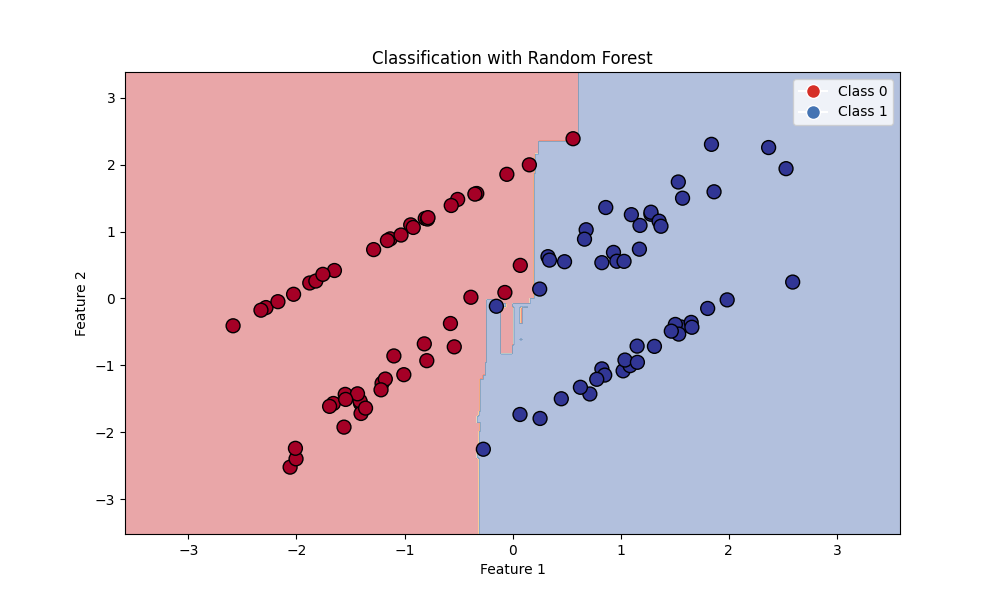
\includegraphics[width=0.8\textwidth]{Master Thesis/Plots/randomForestexample.png}
    \caption{RF separating data points into two classes}
    \label{fig:RF}
\end{figure}
\FloatBarrier

Figure ~\ref{fig:RF} is an example of how classification with RF could look like in a visual case.

\subsection{Boosting as Functional Gradient Descent}

\subsubsection*{Gradient Descent}
Gradient descent is a fundamental algorithm for unconstrained optimization. It iterative updates parameters to minimize a given function \( f(\theta) \). The update rule for gradient descent is given by:
\begin{equation}
    \theta_{k+1} = \theta_k - \eta_k g_k,
\end{equation}
where \( \eta_k \) is the step size or learning rate, and \( g_k \) is the gradient of \( f \) at \( \theta_k \).

Choosing an appropriate step size \( \eta_k \) is crucial because if \( \eta_k \) is too small, the convergence will be very slow.
But if \( \eta_k \) is too large, the algorithm may oscillate or diverge ~\cite{murphy2013machine}.

\subsubsection*{Gradient Boosting}
A more generalized approach, known as gradient boosting, was developed to extend boosting capabilities across various loss functions. It conceptualizes the problem as a functional gradient descent. This builds on the principles of ensemble learning, which have been discussed previously. Ensemble learning involves combining multiple models to improve performance, while boosting is a method that sequentially adjusts the weights of weak learners to minimize errors. It conceptualizes the problem as a functional gradient descent:
\begin{equation}
\hat{f} = \arg\min_{f} L(f)
\end{equation}
Here, $f = (f(x_1), \dots, f(x_d))$ represents the parameters, $f$ is a possible outcome of the ensemble learning method and $L$ represents the loss function. The method updates predictions in a stage wise manner by moving in the direction that reduces the loss function, effectively performing gradient descent in function space. Each update is formulated as:

\begin{equation}
f_m = f_{m-1} - \rho_m g_m
\end{equation}
where $\rho_m$ is the learning rate and $g_m$ is the gradient, optimized as:
\begin{equation}
\rho_m = \arg\min_{\rho \in \mathbb{R}} L(f_{m-1} - \rho g_m)
\end{equation}
The weak learner fits each update to approximate the negative gradient of the loss function, enhancing the model's ability to generalize beyond the fixed set of training points ~\cite{murphy2013machine}.

\subsection{XGBoost}

Extreme Gradient Boosting (XGBoost) is renowned for its efficiency, scalability, and robust handling of sparse data and missing values. It incorporates regularization to prevent overfitting and uses parallel and distributed computing to speed up training. XGBoost's unique features include the 'weighted quantile sketch' for handling weighted data, backward pruning to remove unnecessary splits, and support for custom loss functions. Its built-in cross-validation and feature importance scores aid in model evaluation and interpretation, making it highly effective for large-scale and complex ML tasks.

The ensemble's power is further harnessed through gradient boosting, a technique that evolves in three steps:

\begin{enumerate}
    \item An initial model $F_0$ is formulated to predict the target variable $y$, generating residuals $(y - F_0)$.
    \item A new model $h_1$ is fitted to these residuals.
    \item The model $F_0$ is then updated with $h_1$ to yield a superior model $F_1$, which exhibits a lower mean squared error compared to $F_0$:
\end{enumerate}

\[
F_1(x) \leftarrow F_0(x) + h_1(x)
\]

The process continues by modeling after the residuals of $F_1$ to construct a new model $F_2$, and this iterative process is carried out for 'm' iterations:

\[
F_2(x) \leftarrow F_1(x) + h_2(x)
\]

\[
\vdots
\]

\[
F_m(x) \leftarrow F_{m-1}(x) + h_m(x)
\]

Throughout this iterative process, the additive learners contribute unique information, enhancing the model's accuracy without altering the functions established in the previous steps ~\cite{analyticsvidhyaIntroductionXGBoost}.
The XGBoost can be used for classification and regression. Figure ~\ref{fig:XGBoost} demonstrates the XGBoost for a classification problem:

\FloatBarrier
\begin{figure}[h!]
  \centering
    \centering
    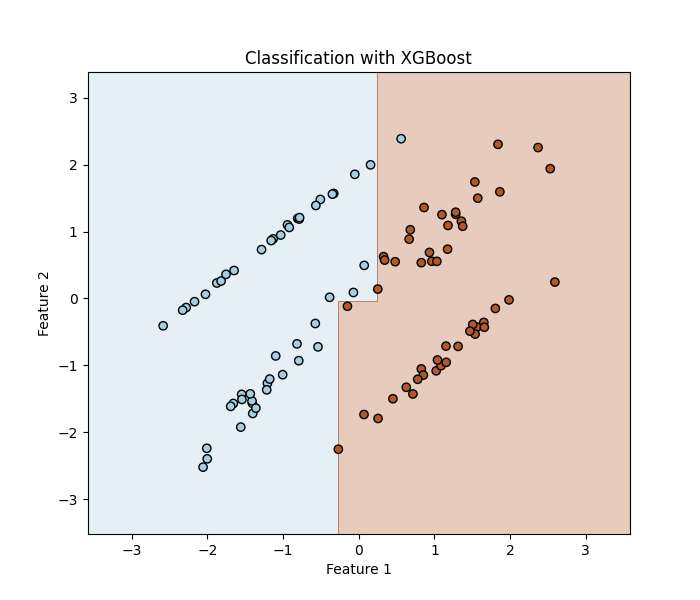
\includegraphics[width=.9\linewidth]{Master Thesis/Plots/classification_with_xgboost.png}
    \caption{XGBoost separating data points into two classes}
    \label{fig:XGBoost}
\end{figure}
\FloatBarrier
We clearly see in figure ~\ref{fig:XGBoost} that XGBoost creates complex decision boundaries for the classification.
This visualization may help later in this work.

\subsection{CatBoost: Gradient Boosting with Decision Trees}
CatBoost is a sophisticated implementation of gradient boosting that utilizes binary decision trees as base predictors. It follows the principles of gradient boosting but introduces several improvements and optimizations for better handling categorical features and preventing overfitting.

The process begins with an initial model \( F_0 \) and iteratively enhances it by fitting subsequent models \( h_t \) to the residuals. CatBoost optimizes this process by employing oblivious decision trees, which apply the same splitting criterion across an entire level of the tree. This leads to more balanced structures and efficient computations.

A decision tree in CatBoost can be defined as:
\begin{equation}
h(x) = \sum_{j=1}^J b_j \mathbbm{1}\{x \in R_j\}
\end{equation}
where \( R_j \) are the disjoint regions of the feature space corresponding to the leaves, and \( b_j \) represents the output value for each region ~\cite{prokhorenkova2019catboost}.

\section{Regression}

\subsection{Logistic Regression}

Logistic regression is a generalization of linear regression for binary classification. Instead of using a Gaussian distribution for the response variable \( y \), we use a Bernoulli distribution since \( y \in \{0, 1\} \). This can be expressed as:
\begin{equation}
    p(y|\mathbf{x}, \mathbf{w}) = \text{Ber}(y|\mu(\mathbf{x})),
\end{equation}
where
\begin{equation}
    \mu(\mathbf{x}) = \mathbb{E}[y|\mathbf{x}] = p(y = 1|\mathbf{x}).
\end{equation}

We compute a linear combination of the inputs, and pass this through the sigmoid function to ensure \( 0 \leq \mu(\mathbf{x}) \leq 1 \):
\begin{equation}
    \mu(\mathbf{x}) = \sigma(\mathbf{w}^T \mathbf{x}),
\end{equation}
where the sigmoid function, also known as the logistic or logit function, is defined as:
\begin{equation}
    \sigma(\eta) = \frac{1}{1 + \exp(-\eta)} = \frac{e^\eta}{e^\eta + 1}.
\end{equation}

Putting these steps together, we get:
\begin{equation}
    p(y|\mathbf{x}, \mathbf{w}) = \text{Ber}(y|\sigma(\mathbf{w}^T \mathbf{x})).
\end{equation}

This is called \textit{logistic regression} due to its similarity to linear regression, although it is a form of classification, not regression.

An example of logistic regression is given by:
\begin{equation}
    p(y_i = 1|x_i, \mathbf{w}) = \sigma(w_0 + w_1 x_i),
\end{equation}
where \( x_i \) is the SAT score of student \( i \) and \( y_i \) indicates whether they passed or failed a class.

The decision rule is defined as:
\begin{equation}
    \hat{y}(\mathbf{x}) = 1 \iff p(y = 1|\mathbf{x}) > 0.5.
\end{equation}

The decision boundary is given by:
\begin{equation}
    \sigma(w_0 + w_1 x) = 0.5 \implies x = x^*.
\end{equation}

Overfitting occurs when a model fits the training data too well, capturing noise instead of the underlying pattern. This can be mitigated by using techniques such as cross-validation and regularization.

Model selection involves choosing the best model from a set of candidates by evaluating their performance on a validation set. This process aims to balance model complexity and accuracy to prevent both overfitting and underfitting ~\cite{murphy2013machine}.

\subsection{Linear Regression}

Regression analysis is very similar to classification. The main difference however is, it is dealing with a continuous response variable ~\cite{murphy2013machine}. Imagine in general having a single real-valued input $x_i \in \mathbb{R}^d$, and a corresponding real-valued response $y_i \in \mathbb{R}$. We explore fitting two models to this data: a linear model (a straight line) and a non-linear model (a quadratic function). The methodologies for fitting these models are discussed subsequently. This simple example can be extended in various ways to include challenges such as high-dimensional inputs, outliers, or non-smooth responses.

Linear regression is one of the most commonly used models in statistical modeling and ML. It posits that the dependent variable, often referred to as the response, is a linear combination of the input variables. The mathematical representation of a linear regression model can be expressed as follows:

\begin{equation}
    f(\mathbf{x}) = \mathbf{w}^T \mathbf{x} + \mathbf{\epsilon} \qquad, \mathbf{w} \in \mathbb{R}^{d} \qquad , \mathbf{x} \in \mathbb{R}^d
\end{equation}

Here, $f(\mathbf{x})$ represents the predicted response for the input vector $\mathbf{x}$, $\mathbf{w}^T \mathbf{x}$ denotes the inner or scalar product of the input vector $\mathbf{x}$ with the model's weight vector $\mathbf{w}$, and $\mathbf{\epsilon}$ symbolizes the residual error, which accounts for the discrepancy between our linear predictions and the actual response. This formula describes the multidimensional case. The equation can be expanded as:

\begin{equation}
    f(\mathbf{x}) = \sum_{j=1}^d w_j x_j + \epsilon_{j}
\end{equation}

where $d$ is the number of features, $w_j$ are the coefficients that represent the weights assigned to each input feature $x_j$, and $\epsilon$ is the error term that captures any factors not explained by the linear model ~\cite{murphy2013machine}.

\FloatBarrier
\begin{figure}[h!]
    \centering
    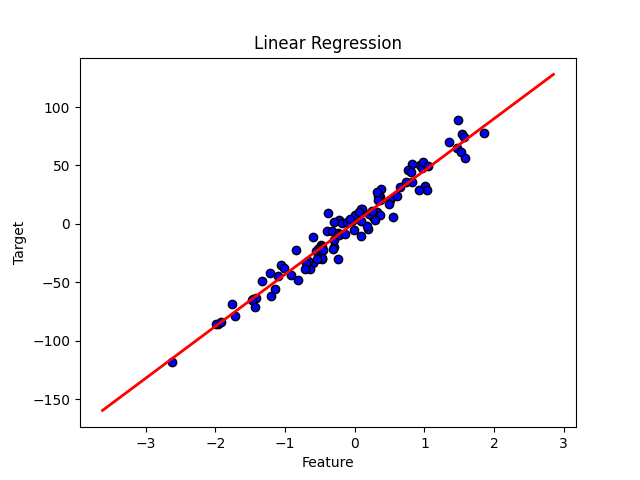
\includegraphics[width=0.7\textwidth]{Master Thesis/Plots/linearregressionexample.png}
    \caption{Linear regression method finding a line trough the data points}
    \label{fig:linreg}
\end{figure}
\FloatBarrier

Figure ~\ref{fig:linreg} is an example of how linear regression could look like in a visual case.

A optimization of this is an approach called boosting. The essence of boosting is to fit adaptive basis-function models, where the functions $\phi_m$ are generated by an algorithm known as a weak learner or a base learner. The algorithm repeatedly applies the weak learner to weighted versions of the data. Initially, all data points are given equal weights, but as the iterations proceed, higher weights are assigned to examples that were incorrectly classified, thus focusing the learning more on harder cases ~\cite{murphy2013machine}.

\section{Artificial Neural Networks}

Artificial Neural Networks (ANNs) are computational models inspired by the human brain, designed to learn complex patterns from data. These networks are composed of layers of interconnected units called neurons, each connection associated with a weight. A prominent type of ANN is the Multilayer Perceptron (MLP), which consists of an input layer, one or more hidden layers, and an output layer. Each layer has neurons connected by weighted links, and the goal is to learn these weights to make accurate predictions.

The MLP can be mathematically represented as follows: For an MLP with \( n \) hidden layers, the function \( F_\theta(x) \) is given by \( F_\theta(x) = f_{n+1}(w_{n+1} f_n(w_n f_{n-1}(\cdots f_1(w_1 x + b_1) + b_2) \cdots + b_{n}) + b_{n+1}) \). Here, \( x \) is the input vector, \( w_i \) are the weight matrices, \( b_i \) are the bias vectors, and \( f_i \) are the activation functions for each layer.

Training an MLP involves adjusting these weights and biases to minimize the error between predicted and actual outputs, using an optimization algorithm like gradient descent. The weight update rule in gradient descent is \( w_{ij}^{(t+1)} = w_{ij}^{(t)} - \eta \frac{\partial L}{\partial w_{ij}} \), where \( \eta \) is the learning rate and \( L \) is the loss function.

Activation functions introduce non-linearity into the model, allowing it to learn complex patterns. Common activation functions include the sigmoid function \( \sigma(x) = \frac{1}{1 + e^{-x}} \) and the ReLU function \( \text{ReLU}(x) = \max(0, x) \) ~\cite{NNs}.

\section{Unsupervised Learning}

Unsupervised learning involves analyzing data without labeled responses, aiming to discover 'interesting structures' within the data, a process often referred to as knowledge discovery. Unlike supervised learning, which requires input-output pairs for training, unsupervised learning focuses on modeling the probability distribution $p(x_i|\phi)$ of the data, without specific targets. Where \(\phi\) represents the parameters of the model that describe the distribution \( p(x_i|\phi) \). These are the unknown parameters that the model adjusts during training to approximate the probability distribution of the data \( x_i \).
This approach is more typical of human and animal learning and is widely applicable, as it doesn't need a human expert to provide labeled data ~\cite{murphy2013machine}.

\subsection{Clustering}

The k-means algorithm works on a set $X$ $\subset$ $\mathbb{R}^d$, which represents an embedding of the vertices. The goal is to find a set of $k$ cluster centers $\mu_C_1$$, \dots ,$$ \mu_C_n$ $\subset$ $\mathbb{R}^d$. The corresponding clusters are then given by 
\begin{equation}
    C_i = {\{x \in X : \lVert x - \mu_{C_i} \rVert}_2 < {\lVert x - \mu_{C_j} \rVert}_2 j \neq i , j\in \{1,\dots ,k\}\}
\end{equation}

If a point is on the boundary between two clusters, it is randomly assigned to one of the adjacent clusters.
We start with a random set of cluster centers and calculate their corresponding clusters.
After that, we calculate new cluster centers from the obtained clusters like 
\begin{equation}
    \mu_{C_i} = \Big(\,\frac{1}{|C_i|}\Big)\,\sum_{x \in C_i}x
\end{equation} 
where $i \in \{1, \dots, k\}$.
We repeat this process until the clusters do not change.
For the k-means algorithm we have a set $X$ consisting of data points and a set $\mu_C$ $\subset$ $V$ representing the centers ~\cite{murphy2013machine}. 

\FloatBarrier
\begin{figure}[h!]
    \centering
    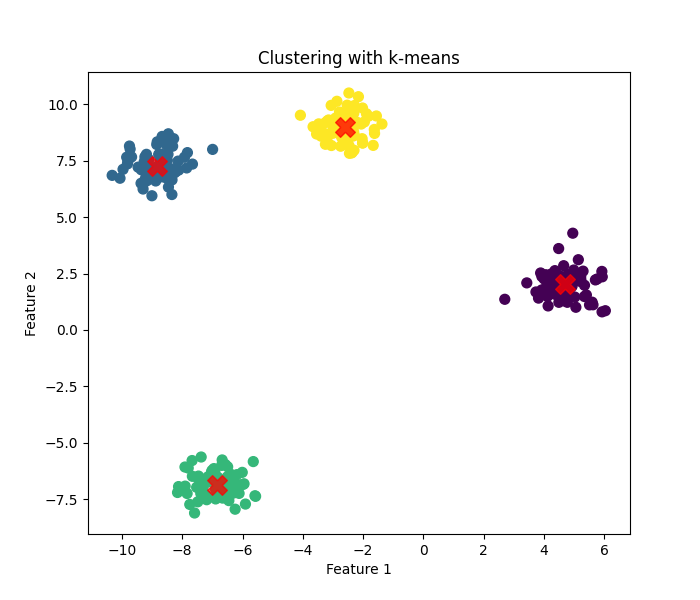
\includegraphics[width=0.7\textwidth]{Master Thesis/Plots/Clustering_Example.png}
    \caption{Method k-means clustering the data points into four clusters}
    \label{fig:clustering}
\end{figure}
\FloatBarrier

Figure ~\ref{fig:clustering} shows the results of a k-means clustering model that groups data points into four clusters. The differences to the previous plots of the methods are that this plot does not show decision boundaries, but the grouping of the data points into clusters.

\subsection{Hierarchical Clustering}

Hierarchical clustering is a method of cluster analysis which seeks to build a hierarchy of clusters. This approach can be categorized into two main types: agglomerative (bottom-up) and divisive (top-down).

Agglomerative clustering, or bottom-up clustering, starts with each object in a singleton cluster. The clusters are iteratively merged based on their similarity until a single cluster containing all objects is formed. 

Initially, each data point \( x_i \) is treated as a singleton cluster \( C_i = \{i\} \). At each step, the two most similar clusters \( C_j \) and \( C_k \) are identified and merged to form a new cluster \( C_\ell = C_j \cup C_k \). The similarity \( d_{jk} \) between clusters is determined using a dissimilarity matrix. After merging \( C_j \) and \( C_k \) into \( C_\ell \), the dissimilarity matrix is updated to reflect the distances between the new cluster \( C_\ell \) and the remaining clusters. Different linkage criteria can be used to define the distance between clusters: 

\textit{Single Linkage}: 
\[ d(C_\ell, C_i) = \min \{d(x_p, x_q) | x_p \in C_\ell, x_q \in C_i\} \]

\textit{Complete Linkage}: 
\[ d(C_\ell, C_i) = \max \{d(x_p, x_q) | x_p \in C_\ell, x_q \in C_i\} \]

\textit{Average Linkage}: 
\[ d(C_\ell, C_i) = \frac{1}{|C_\ell||C_i|} \sum_{x_p \in C_\ell} \sum_{x_q \in C_i} d(x_p, x_q) \]

where $x_p$ and $x_q$ are data points in clusters $C_\ell$ and $C_i$ respectively. This criterion measures the minimum distance between any pair of points in the two clusters.
 
The process is repeated until all points are merged into a single cluster or the desired number of clusters is achieved.

The algorithm for divisive clustering can be summarized as follows:

\FloatBarrier
\begin{algorithm}
\caption{Agglomerative clustering}
\begin{algorithmic}[1]
\State initialize clusters as singletons: for \(i \leftarrow 1\) to \(n\) do \(C_i \leftarrow \{i\}\);
\State initialize set of clusters available for merging: \(S \leftarrow \{1, \ldots, n\}\);
\Repeat
\State Pick 2 most similar clusters to merge: \((j, k) \leftarrow \arg \min_{j,k \in S} d_{jk}\);
\State Create new cluster \(C_\ell \leftarrow C_j \cup C_k\);
\State Mark \(j\) and \(k\) as unavailable: \(S \leftarrow S \setminus \{j, k\}\);
\If {$C_\ell \neq \{1, \ldots, n\}$} 
\State Mark \(\ell\) as available, \(S \leftarrow S \cup \{\ell\}\);
\ForAll {$i \in S$}
\State Update dissimilarity matrix \(d(i, \ell)\);
\EndFor
\EndIf
\Until {no more clusters are available for merging};
\end{algorithmic}
\end{algorithm}
\FloatBarrier

Divisive clustering, or top-down clustering, works in the opposite manner. It starts with all data points in a single cluster and recursively splits them into smaller clusters. This approach is less commonly used due to its computational complexity ~\cite{murphy2013machine}.

Hierarchical clustering provides a comprehensive way to understand the structure within data by creating nested clusters. The choice between agglomerative and divisive methods, as well as the linkage criteria, can significantly impact the resulting hierarchy and its interpretation ~\cite{murphy2013machine}.

\section{Metrics}

To evaluate the performance of classification models in data science and ML, the three metrics precision (p), recall (r) and the f1-score are particularly useful. 
In general when we need to define that TP stands for true positive, FP for false positive and FN for false negative. 

Precision tells us how many of the cases classified as positive are actually positive. For example, we have a group of healthy and sick people and use a program that classifies as either 'healthy' or 'sick'. Precision is then calculated as follows: Of all the people classified as 'sick', how many are actually sick? Described as a mathematical formula it would look like this ~\cite{10.1007/978-3-540-31865-1_25}: 

\begin{equation}
    p = \frac{TP}{TP + FP}
\end{equation}

Recall measures how well the model has captured all actual positive cases. In the example with the healthy and sick people program, this would be: Of all really sick people, how many did the program correctly identify as 'sick'? Mathematically this would be ~\cite{10.1007/978-3-540-31865-1_25}: 

\begin{equation}
    r = \frac{TP}{TP + FN}  
\end{equation}

If you want to measure the balance between precision and recall in a single metric, one can use the f-score. It is particularly useful if a balanced relationship between precision and recall is to be achieved. The f-score is, so to speak, the weighted harmonic average of precision and recall. A higher f-score indicates a better overall performance of the model.
~\cite{10.1007/978-3-540-31865-1_25}:

\begin{equation}
    f_\beta = (1 + \beta^2) \frac{p \cdot r}{(r + \beta^2 p)} \qquad , \beta \in [0 , 1]
\end{equation}

Where $\beta = 1$ represents the f1 score.

The silhouette score is a measure of how similar an object is to its own cluster compared to other clusters. The silhouette scores ranges from $[-1 ,1]$, where a higher value indicates that the object is well matched to its own cluster. The silhouette score of a data point $x$ is given as ~\cite{SilhotteCoefficient}:
\begin{equation}
     s(i) = \frac{b(x) - a(x)}{max\{a(x),b(x)\}}
\end{equation}
with $b(x)$ denoting the mean distance to all other points of the next nearest cluster, and $a(x)$ is the mean distance to all other points of the same cluster. 
The silhouette score for a set of samples is then defined as :
\begin{equation}
    s_C = \frac{1}{n_C} \sum_{x \in C} s(x)
\end{equation}
the mean of the silhouette score for each sample.

Before we introduce \( R^2 \) in this work, we need to mention residuals. 
Residuals are the differences between the observed values \( y_i \) and the predicted values \( \hat{y}_i \) produced by the regression model. Mathematically, the residual for each observation \( i \) is given by ~\cite{Weisberg}:

\[
\text{residual}_i = y_i - \hat{y}_i
\]

The residual sum of squares (\( \text{SS}_{\text{res}} \)) is then calculated by summing the squares of these residuals for all observations:

\[
\text{SS}_{\text{res}} = \sum_{i=1}^{n} (y_i - \hat{y}_i)^2
\]

This measure indicates the extent to which the predicted values differ from the actual observed values. A smaller \( \text{SS}_{\text{res}} \) implies that the model's predictions are closer to the actual data points, indicating a better fit.

The term \(\text{SS}_{\text{tot}}\) refers to the total sum of squares, which measures the total variance in the observed data. It is calculated by summing the squares of the differences between each observed value and the mean of the observed values \(\bar{y}\):

\[
\text{SS}_{\text{tot}} = \sum_{i=1}^{n} (y_i - \bar{y})^2
\]

This term represents the total variation present in the data, without considering the regression model.

Now the coefficient of determination \( R^2 \) can be introduced. It quantifies the proportion of the variance in the dependent variable that is predictable from the independent variables. It is given by ~\cite{Weisberg}:

\[
R^2 = 1 - \frac{\text{SS}_{\text{res}}}{\text{SS}_{\text{tot}}}
\]

An \( R^2 \) value of 1 indicates that the regression model perfectly explains the variance in the data, while an \( R^2 \) value of 0 indicates that the model does not explain any of the variance in the data.

We also used MSE in this work to find out the fact how far apart the real value and the predicted value are. It is calculated like this:
\[
\text{MSE} = \frac{1}{n} \sum_{i=1}^{n} (y_i - \hat{y}_i)^2
\]
This measures the average of the squares of the errors (residuals), which are the differences between the observed values \(y_i\) and the predicted values \(\hat{y}_i\).

Some other measurement is the root-mean-square error (RMSE). It provides a measure of the average magnitude of the prediction error. It is calculated as the square root of the average squared differences between the predicted and actual values:

\[
\text{RMSE} = \sqrt{\frac{\sum_{i=1}^n (y_i - \hat{y}_i)^2}{n}}
\]

\subsection{Cross Entropy}

To measure the differences between two discret probability distributions, p and q, the Kullback-Leibler divergence or relative entropy is often used. 
Mathematically it can be described like this ~\cite{murphy2013machine}: 
\begin{equation}
    \mathbb{KL}(p||q) \equiv \sum_{k=1}^{K} p_k \log \frac{p_k}{q_k}
\end{equation}
where the sum is given by an integral for probability distribution functions. It can be rewritten as:
\begin{equation}
   \mathbb{KL}(p||q) = \sum_k p_k \log p_k - \sum_k p_k \log q_k = -\mathbb{H}(p) + \mathbb{H}(p, q)
\end{equation}
Where $\mathbb{H}(p, q)$ is called the cross entropy (CE).

\begin{equation}
    \mathbb{H}(p, q) \equiv -\sum_k p_k \log q_k
\end{equation}

The CE method is mainly used for combinatorial and multi-extreme optimization as well as for the simulation of rare events. 
With the CE method, a random data sample is generated in each iteration. The parameters of the random mechanism are then updated on the basis of this data in order to generate a 'better' sample in the next iteration. The method uses the Kullback-Leibler distance to minimize the distance between the current estimate and the optimal solution.
This guarantees a more precise estimate of the probabilities searched for ~\cite{crossentropy1}.

\subsection{Silhouette Score and Davies-Bouldin Score}

The silhouette score is a measure of how similar an object is to its own cluster compared to other clusters. The silhouette scores ranges from $[-1 ,1]$, where a higher value indicates that the object is well matched to its own cluster. The silhouette score of a data point x is given as:
\begin{equation}
     s(i) = \frac{b(x) - a(x)}{max\{a(x),b(x)\}}
\end{equation}
with $b(x)$ denoting the mean distance to all other points of the next nearest cluster, and $a(x)$ is the mean distance to all other points of the same cluster. 
The silhouette score for a set of samples is then defined as :
\begin{equation}
    s_C = \frac{1}{n_C} \sum_{x \in C} s(x)
\end{equation}
the mean of the silhouette score for each sample ~\cite{SilhotteCoefficient}.

The Davies-Bouldin score is a measure used to evaluate the quality of clustering by assessing the similarity between clusters. It quantifies how well-separated and compact the clusters are within a dataset. The Davies-Bouldin score is defined based on the following components:

Firstly, the dispersion measure (\( S_i \)) for a cluster \( C_i \) is calculated to determine the spread of data points within the cluster. This is given by:
\[ 
S_i = \left( \frac{1}{|C_i|} \sum_{x \in C_i} \| x - A_i \|^2 \right)^{1/2} 
\]
where \( A_i \) is the centroid of cluster \( C_i \).

Secondly, the separation measure (\( M_{ij} \)) between clusters \( C_i \) and \( C_j \) is determined by the distance between their centroids:
\[ 
M_{ij} = \| A_i - A_j \| 
\]

Using these measures, the similarity measure (\( R_{ij} \)) between clusters \( C_i \) and \( C_j \) is defined as:
\[ 
R_{ij} = \frac{S_i + S_j}{M_{ij}} 
\]

The Davies-Bouldin score for a set of clusters is then calculated as the average similarity of each cluster with its most similar cluster:
\[ 
DBI = \frac{1}{d} \sum_{i=1}^{d} \max_{j \neq i} R_{ij} 
\]
where \( d \) is the total number of clusters.

A lower DBI indicates better clustering performance, with well-separated and compact clusters, while a higher DBI suggests poorer clustering with less distinct clusters. The DBI is effective for comparing the quality of different clustering algorithms or parameter settings and is applicable to datasets of arbitrary dimensionality. This measure requires minimal user interaction and is computationally feasible for large datasets, making it a valuable tool for automated clustering evaluation
~\cite{4766909}.

We have now defined and explained all the methods and metrics that are relevant to the following sections of this paper. By establishing a clear understanding of these techniques, we are now in a position to proceed with the analysis and evaluation of our data. Based on this, we can fully evaluate the effectiveness of different ML approaches in health monitoring and prediction.
\chapter{Example Dataset}
\label{cha:exampleDataset}

In this chapter, we delve into the structure of the dataset on an example to simplify its extraction and usage later in this work. We will primarily focus on the data the Apple Watch can provide, highlighting key metrics such as heart rate, distance, step count and other relevant physiological and activity parameters. This includes showcasing the various types of information the Apple Watch tracks and identifying which pieces of information are crucial for this work.

\section{Structure of the Dataset}

The dataset consists of recorded Apple Watch values. A total of two people of each sex were wearing the smartwatch over a period of two years. During this time, a wide variety of values were collected. Initially, the data were exported in Extensible Markup Language (XML) format and were converted into Comma-Separated Values (CSV) tables using the implemented program to simplify data usage. 

CSV files are often preferred over XML for data handling in Python due to their simplicity, readability, and performance. CSV files consist of plain text, making them easy to read and parse, whereas XML files have a more complex structure with nested tags. Parsing CSV files is faster and more efficient, especially for large datasets, thanks to Python's robust libraries like 'pandas' and the built-in 'csv' module. These libraries provide convenient functions for handling CSV data.

Our converted CSV table consists of 38 columns, but this study primarily used only the columns 'type', 'value', 'unit', 'startDate' and 'endDate', so five columns in total and all measured data categories are already listed in the 'type' column.

We are not using any other columns, because the other columns were mostly not measured correctly or not measured at all and therefore did not provide sufficient data. 

The 'type' column refers to the type of recording, for example, whether the watch recorded a running session, the calories burned, or the person's heart rate. The 'value' column stores all measured values, and the 'unit' column represents the corresponding unit, such as minutes, kilometers, calories, etc. The 'startDate' and 'endDate' columns are particularly important for determining the exact interval of the recording.

\section{Heart Rate, Energy Burned and Walked Distance Analysis}

We started by filtering all entries in the 'type' column of the CSV table labeled 'HeartRate,' with a particular focus on the 'value' 32.

\subsection{Daily Behavior and Correlations in the Example Dataset}
We selected the day with the highest heart rate and filtered all the data from that day, such as heart rate, calories burned and distance traveled, to see how the high heart rate relates to other features. This resulted in the following graphs for two healthy individuals:

\FloatBarrier
\begin{figure}[h!]
  \centering
  \begin{minipage}[b]{0.8\linewidth}
    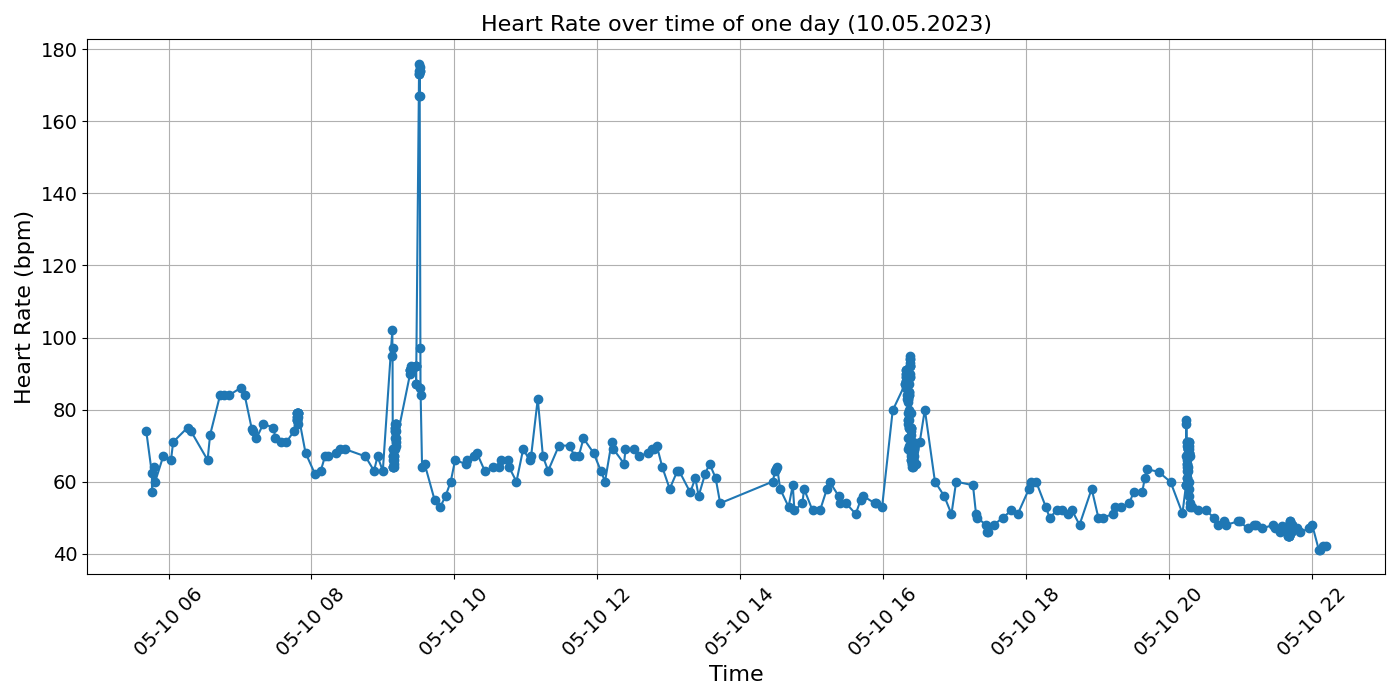
\includegraphics[width=\linewidth]{Master Thesis/Plots/HeartRate1day_Michi.png}
    \caption{Day of maximal heart rate in a male subject over 30 years of age}
    \label{fig:MaxHeartMichi}
  \end{minipage}
  \quad % Fügt etwas Platz zwischen den Bildern ein
  \begin{minipage}[b]{0.8\linewidth}
    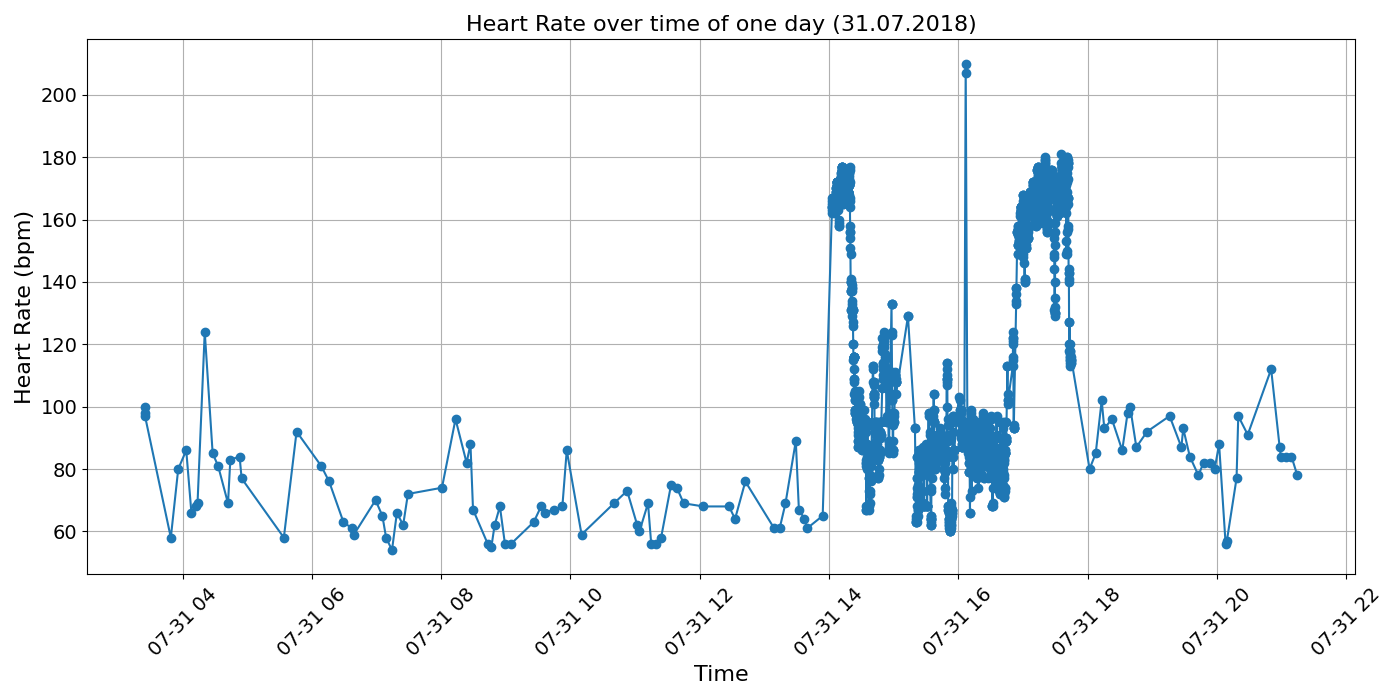
\includegraphics[width=\linewidth]{Master Thesis/Plots/HeartRate1day_Tanja.png}
    \caption{Day of maximal heart rate in a female test subject under 25 years of age}
    \label{fig:MaxHeartTanja}
  \end{minipage}
\end{figure}
\FloatBarrier

The provided figures ~\ref{fig:MaxHeartMichi} and ~\ref{fig:MaxHeartTanja} show heart rate data over the course of one day for two subjects. The first plot represents the heart rate of a subject over 30 years of age on May 10, 2023. The second plot illustrates the heart rate of a subject on July 31, 2018.

The young female subject exhibits significant variations in heart rate throughout the day, with notable peaks between 2 PM and 6 PM reaching up to 201 bpm, and a minimum of 54 beats per minute (bpm). The subject in the 30 to 35 years age range shows a more stable heart rate pattern, with a maximum of 176 bpm and a minimum of 41 bpm.

So far, the analysis of the dataset focused solely on heart rate. It becomes particularly interesting when we include additional factors in our examination. For this reason, we chose the types 'BasalEnergyBurned', 'ActiveEnergyBurned', and 'HeartRate'. The feature 'BasalEnergyBurned' refers to a type of sampling that measures the time the user has spent on activities during the specified day, including whole-body movements ~\cite{appleBasalEnergyBurnedApple}.
The feature 'ActiveEnergyBurned' is the energy the user burned due to physical activity and movement. These samples should not include the resting energy burned during the sample duration ~\cite{appleActiveEnergyBurnedApple} and 'HeartRate' is the pulse measurement ~\cite{appleHeartRateApple}. After selecting the types, the focus was again on the day with the highest bpm value.

\FloatBarrier
\begin{figure}[h!]
  \centering
    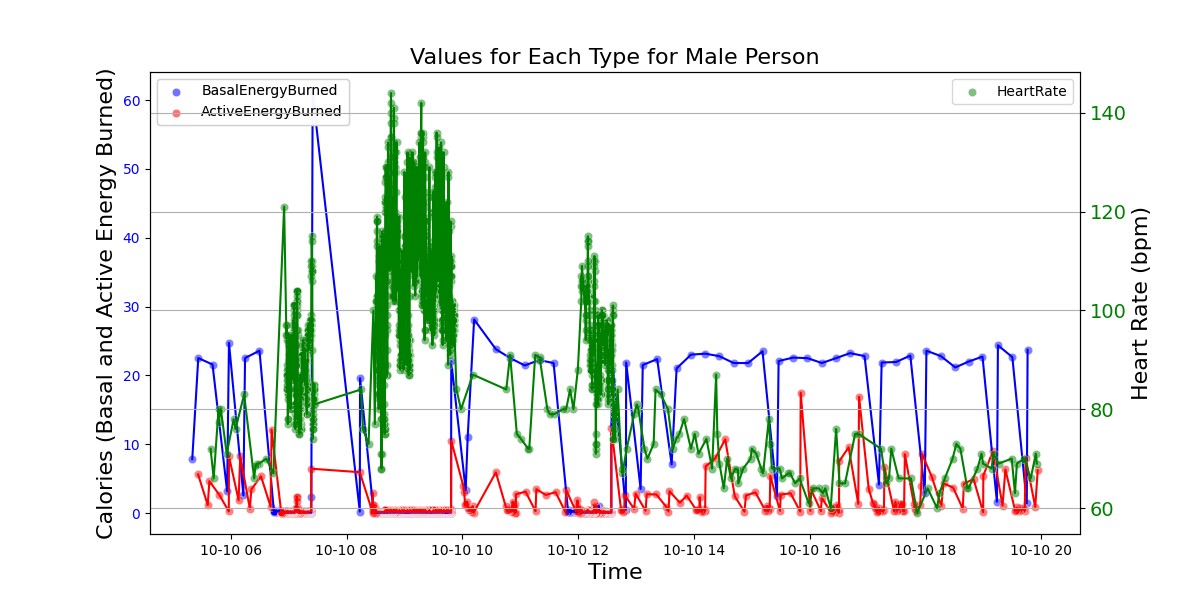
\includegraphics[width=1.0\textwidth]{Master Thesis/Plots/Values_Mean_Male.png}
    \caption{Day of maximal heart rate in a male subject over 30 years of age all relevant values}
    \label{fig:ValuesMale}
    \end{figure}
\FloatBarrier

\FloatBarrier
\begin{figure}[h!]
  \centering
    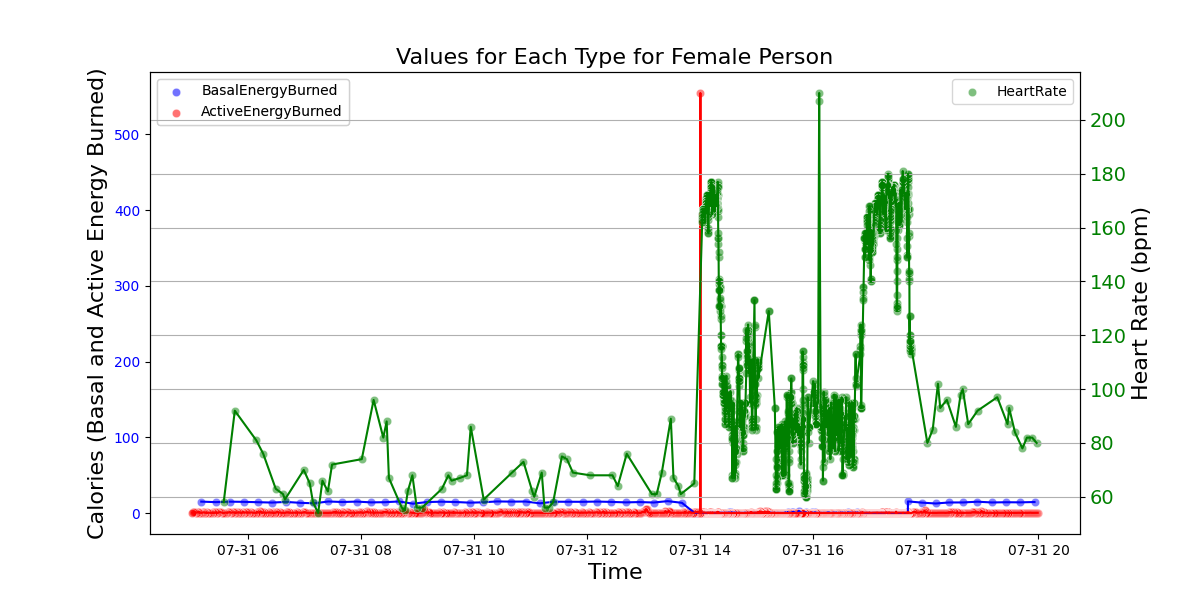
\includegraphics[width=1.0\textwidth]{Master Thesis/Plots/Values_Mean_Female.png}
    \caption{Day of maximal heart rate in a female test subject under 25 years of age all relevant values}
    \label{fig:ValuesFemale}
\end{figure}
\FloatBarrier

The key observations of figure ~\ref{fig:ValuesMale} and figure ~\ref{fig:ValuesFemale} are that the older male subject shows less variation in heart rate and energy burned, possibly indicating a more sedentary lifestyle or a more controlled and steady day of activities.
The younger female subject exhibits extreme heart rate values that are likely to be because of extreme stress or physical activity.
The relationship between heart rate and energy burned is not directly apparent in these plots, suggesting that individual physical responses and activities may vary widely.
In both plots, the exact times of day when heart rate and energy expenditure peak could be further analyzed to understand the subjects activity patterns and potential health implications, but we will leave that at this point of the work.

\subsection{Weekly Behavior and Correlations in the Example Dataset}

At this stage of the thesis, only the day with the highest bpm value has been taken into consideration. In order to be able to make better statements and analyze abnormalities, we want to look at a whole week of the test subjects. As the plots for this are very difficult to read and analyze, the days of the week 25.07 to 31.07 were added together and the average of these days was then calculated. 
It should also be mentioned that we did not consider the steps but the distance covered by the test subjects as we do not know the exact step size. 
The results can be seen in the following table: 

\FloatBarrier
\begin{table}[h!]
\centering
\begin{tabular}{|l|c|r|}
\hline
\textbf{feature} & \textbf{female 20 - 25 years } & \textbf{male  30 - 35 years} \\ \hline
avg. heart rate      & 99.89 bpm         &  76.89 bpm       \\ \hline
avg. active energy burned      & 1620.24 kcal         & 836.19 kcal       \\ \hline
avg. basal energy burned & 1362.89 kcal         & 2045.07 kcal      \\ \hline
avg. distance walking running      & 18.54 km         & 15.67 km     \\ \hline
\end{tabular}
\caption{Table of important characteristics with the average value in a particular week}
\label{table:example}
\end{table}
\FloatBarrier

It is now noticeable again that the female test subject has a higher pulse rate on average than the male test subject. Besides, this is probably mainly due to the age category. One discrepancy that is particularly noticeable is, that the female test subject has a significantly higher average calorie consumption in relation to actively consumed calories. Although, their basal energy burned value is almost the same. This value is very different for the male test subject. On the other hand, we see a higher value for the average kilometers covered per day this week for the male subject, but both exceed the recommended daily distance of 8 km. This is generally a satisfactory result.

\subsection{Exploring the Example Dataset with Cross Entropy}

Initially, the focus of the study was on heart rate, as this, along with calories burned, is most commonly recorded.
But how do we manage to compare the two sex and their distributions effectively without just relying on our eyes? 

To gain a detailed understanding of the heart rate and its measurement, all available values were first illustrated in a graph.
This is where cross-entropy comes into play. In the following, this methodology was applied to the four features.

\FloatBarrier
\begin{figure}[h!]
  \centering
  \begin{subfigure}{.55\textwidth}
    \centering
    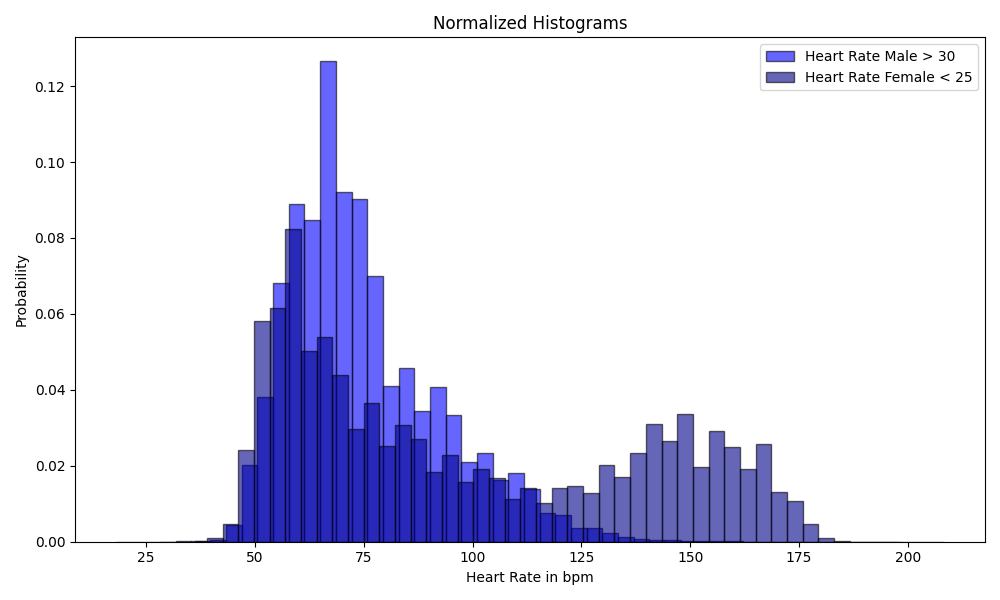
\includegraphics[width=.8\linewidth]{Master Thesis/Plots/CrossEntro_HeartRate.png}
    \caption{Distributions of heart rates of male and female subject}
    \label{fig:heart_rate}
  \end{subfigure}%
  \begin{subfigure}{.55\textwidth}
    \centering
    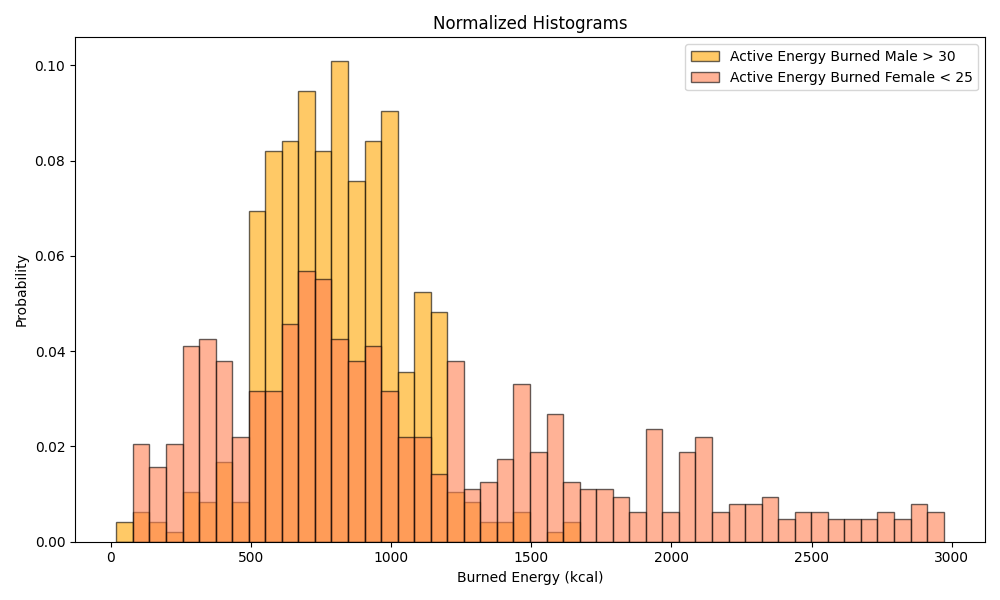
\includegraphics[width=.8\linewidth]{Master Thesis/Plots/CrossEntro_ActiveEnergyBurned.png}
    \caption{Distributions of active energy burned of male and female subject}
    \label{fig:active_energy}
  \end{subfigure}
  \newline
  \begin{subfigure}{.55\textwidth}
    \centering
    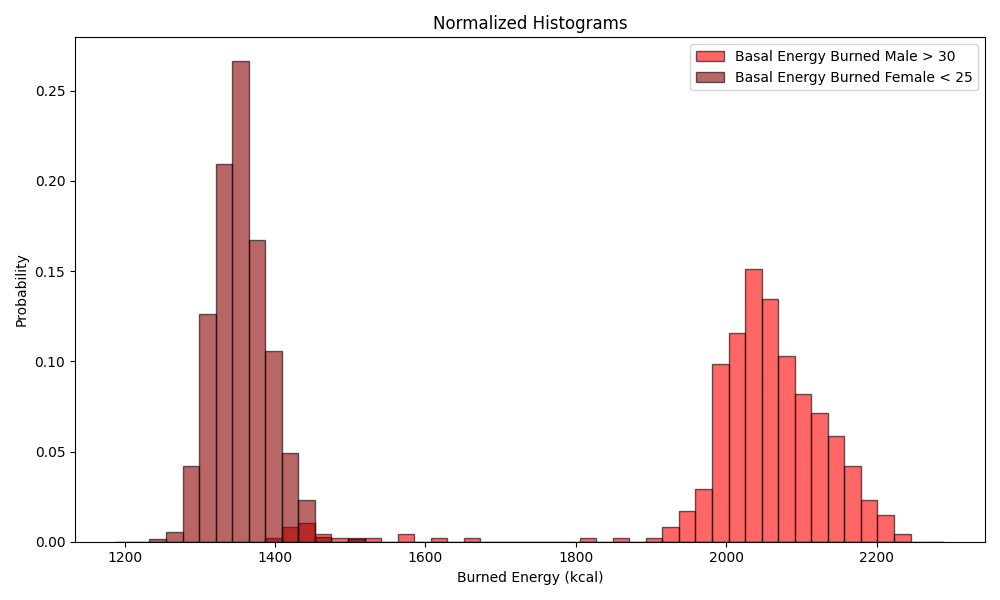
\includegraphics[width=.8\linewidth]{Master Thesis/Plots/CrossEntro_BasalEnergyBurned.png}
    \caption{Distributions of basal energy burned of male and female subject}
    \label{fig:basal_energy}
  \end{subfigure}%
  \begin{subfigure}{.55\textwidth}
    \centering
    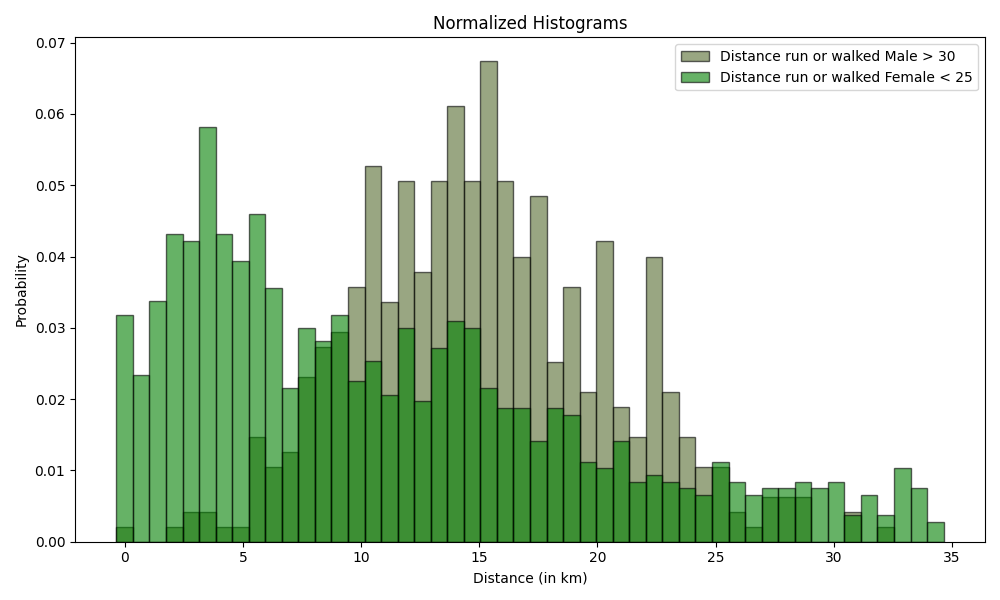
\includegraphics[width=.8\linewidth]{Master Thesis/Plots/CrossEntro_Distance.png}
    \caption{Distributions of walked or jogged distances of male and female subject}
    \label{fig:distance}
  \end{subfigure}
  \caption{Distributions for different data types of the example dataset}
  \label{fig:cross_entropy}
\end{figure}
\FloatBarrier

The presented plots in ~\ref{fig:cross_entropy} illustrate the distributions of various measurements for male and female subjects. The histograms depict how heart rate, active energy burned, basal energy burned, and walked or jogged distances differ between the two subjects.

In the first plot ~\ref{fig:heart_rate}, the distributions of heart rates for male and female subjects are shown. The plot reveals that the heart rates of female subjects (in blue) are generally higher than those of male subjects (in lighter blue). Notably, the heart rate distribution of female subjects is concentrated between 60 and 90 bpm (beats per minute).

The second plot ~\ref{fig:active_energy} displays the distributions of active energy burned for male and female subjects. The distribution for male subjects (yellow) tends to be higher than that for female subjects (orange). This may indicate that male subjects engaged in more intensive physical activities during the tests.

The third plot ~\ref{fig:basal_energy} represents the distributions of basal energy burned for male and female subjects. Again, a clear distinction between sex is observed. The distribution for female subjects (dark red) is generally lower than that for male subjects (red), which may reflect differences in basal metabolic rate and metabolism.

The fourth plot ~\ref{fig:distance} shows the distributions of walked or jogged distances for male and female subjects. It is evident that female subjects (green) generally covered shorter distances compared to male subjects (dark green). This could indicate differences in physical activity levels and endurance.

\newpage

Overall, it is clear that none of the distributions are identical. To quantify this more precisely, the cross-entropy value was calculated, as described in chapter ~\ref{cha:methods}. 

The best results were obtained for 'ActiveEnergyBurned' at 3.48, 'HeartRate' at 3.57, and 'DistanceWalkingRunning' at 3.95. These values suggest that these distributions are the most similar, although they are still far from 1, which would indicate an ideally identical or nearly identical distribution. For 'BasalEnergyBurned' at 33.70, the worst result was obtained, and a quick glance shows that these distributions are completely different.


\chapter{Analyzing the Study Dataset}
\label{cha:studyDataSet}

In this chapter, we explain the whole process of data extraction, focusing on the key aspects of the study dataset. Before we discuss the implementation and results, it's important to understand the preparation process, the distributions of the data features and their entropy. It is crucial to identify the main features, and talk about why certain features are more important and were included but others not.

\section{Data Preparation and Preprocessing}

The structure of the study dataset closely resembles that described in chapter ~\ref{cha:exampleDataset}. Consequently, the initial approach was once again identical. We began by converting the XML file into a CSV table before proceeding with further preparations. 

We have two XML files that are available to us. One is the 'export.xml' file and the other is the 'export\_cda.xml' file. First, we convert both into CSV tables and then consider whether we want to use both. After a closer look, we realize that in the clinical document architecture (CDA) document, the first five of the ten columns have identical entries per column throughout. We therefore consider these to be unusable but used the columns 'DisplayName', 'MeasurementValue', 'Unit' and 'EffectiveTime'. The mentioned CDA columns, contain information on the height, weight and heart rates of the test subjects. The information is also provided with a time stamp, which makes it easier to ensure a comparison with the other data and to simplify the subsequent merging of the tables. 

The converted export file, on the other hand, consists of 36 columns. Of the 36 columns, 29 are empty and therefore unusable. The remaining columns provide information such as 'type', 'value', 'unit', 'startDate', 'endDate', and 'creationDate', as mentioned in chapter ~\ref{cha:exampleDataset}. We therefore re-extracted the table and removed all columns except for the six aforementioned ones.

In addition to the 'export' and 'export\_cda' files, we were given access to a Google shared document titled '6MWT\_Test\_Runs'. In this document, a study supervisor documented important information during the data collection process. This provided us with essential details such as the 'study ID', 'height', 'weight', 'age', 'leg length', and entries in the 'Subject/Patient' column, indicating whether the participant was healthy or a patient. Additionally, the document contains information about all other electronic devices used for the measurements and the data they collected. However, we focused exclusively on data related to the Apple Watch Ultra. Specifically, we filtered and utilized the columns 'Distance (km)', 'Steps (before)', 'Steps (after)', and 'Steps'. The shared document consists of four relevant sheets.

Next, we needed to merge the export file with the '6MWT\_Test\_Runs' document to make the most of all available and relevant information. We initially looked for a unique function to combine the tables effectively. Despite several attempts, this approach was unsuccessful. Eventually, we found that the combination of height, weight and the time stamp served as the best criteria for merging the datasets. This process was done manually since the shared document recorded height and weight with precise decimal values, whereas the Apple Watch Ultra rounded these.

We ensured accuracy by verifying that entries in the shared document were recorded chronologically, starting with the first participant and continuing in sequence, matching the temporally sorted data collected by the Apple Watch Ultra. This cross-verification allowed us to merge the tables as accurately as possible. Any participants for whom a match could not be found were removed from the dataset. This meticulous process ensured that the merged dataset was comprehensive and precise, setting a solid foundation for further analysis.

Finally, we performed fine-tuning of the dataset. Initially, we worked with three heart rate values per participant: the lowest, highest, and average heart rates. These values were sequentially added to new columns, labeled as 'Heart Rate 1' to 'Heart Rate 3'. This approach ensured that the dataset was optimally prepared for further analysis.

\subsection{Visual Heart Rate Analysis}

We selected the day with the highest heart rate for both a male and a female subject and filtered all the heart rate data from that day during the 6 MWT. This analysis resulted in the following graphs for two healthy individuals:

\FloatBarrier
\begin{figure}[h!]
  \centering
  \begin{minipage}[b]{0.8\linewidth}
    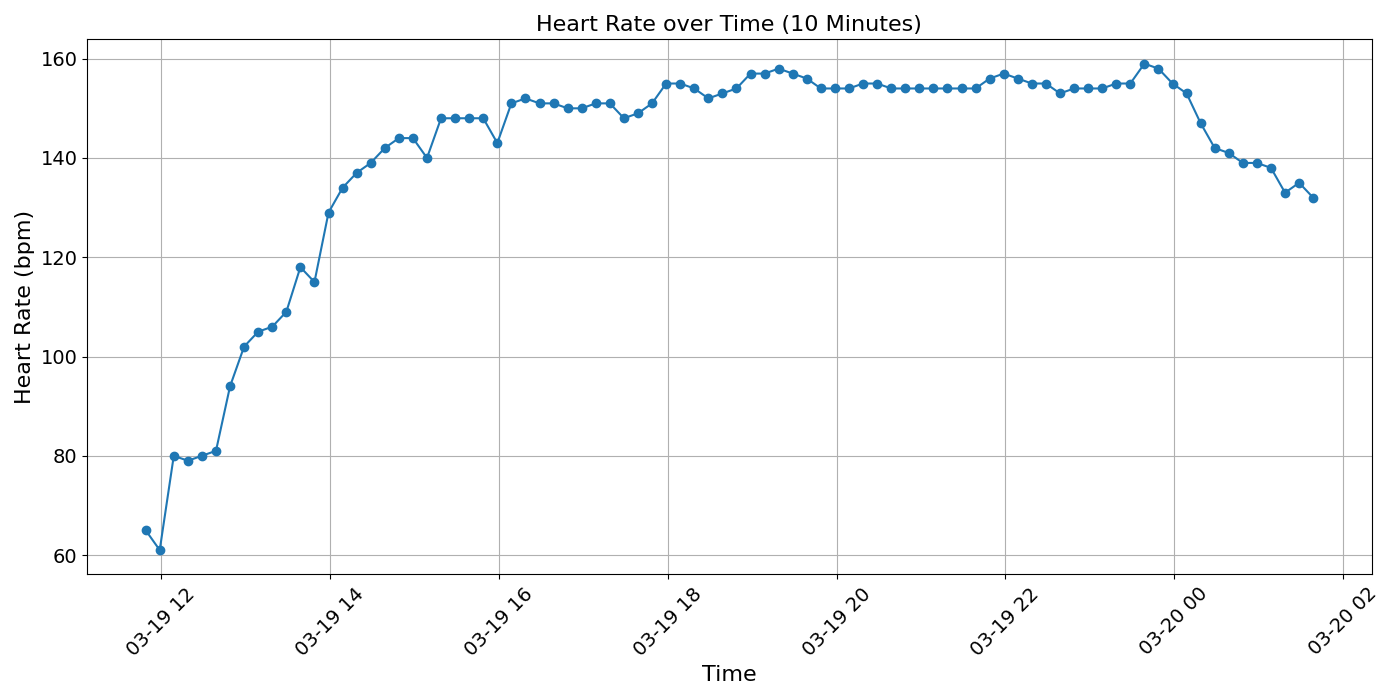
\includegraphics[width=\linewidth]{Master Thesis/Plots/HeartRate1day_Subject_male.png}
    \caption{Day of maximal heart rate in a male subject}
    \label{fig:maxheartorigmale}
  \end{minipage}
  \quad % Fügt etwas Platz zwischen den Bildern ein
  \begin{minipage}[b]{0.8\linewidth}
    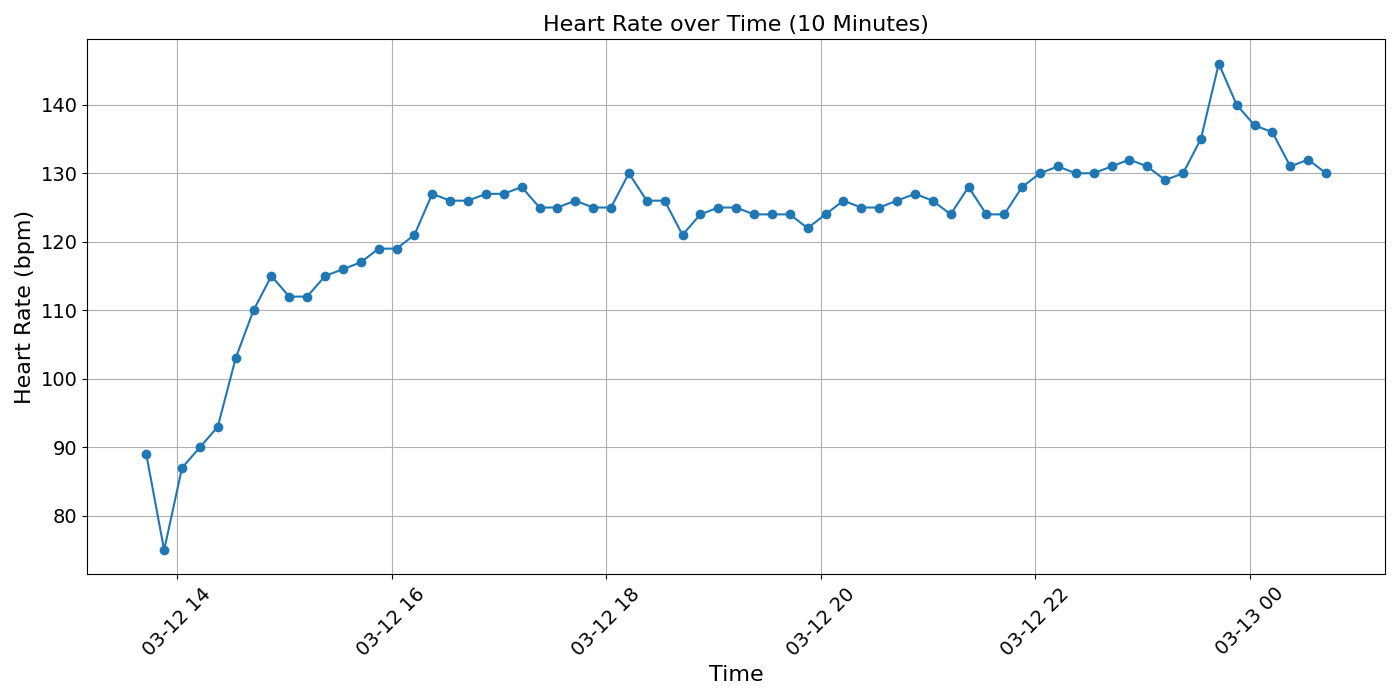
\includegraphics[width=\linewidth]{Master Thesis/Plots/HeartRate1day_Subject_female.png}
    \caption{Day of maximal heart rate in a female subject}
    \label{fig:maxheartorigfemale}
  \end{minipage}
\end{figure}
\FloatBarrier

The two figures ~\ref{fig:maxheartorigmale} and ~\ref{fig:maxheartorigfemale} displayed illustrate the heart rate variations over a 10-minute interval for two subjects, each on their day of maximal recorded heart rate, to ensure we see the heart rate before and after the 6MWT as well. These plots provide insights into the heart rate trends and highlight the differences in cardiovascular response between the subjects.

Figure ~\ref{fig:maxheartorigmale} represents the heart rate data for a male subject over 30 years of age. The heart rate starts at around 60 bpm and shows a steady increase, reaching a peak of approximately 160 bpm. After reaching the peak, the heart rate stabilizes at this high level for a while before gradually decreasing towards the end of the 10-minute interval.

Figure ~\ref{fig:maxheartorigfemale} depicts the heart rate data for a female subject over 25 years of age. The heart rate begins at around 80 bpm and steadily rises, peaking at approximately 140 bpm. Similar to the male subject, her heart rate maintains a high level for a period before it starts to decline towards the end of the interval.

\subsection{BMI as an Additional Feature}

The initial analysis revealed that determining sex based solely on the two given features proved challenging. This prompted an exploration of alternative methods, such as calculating the BMI, to facilitate a more accurate categorization.

\FloatBarrier
\begin{figure}[h!]
\centering
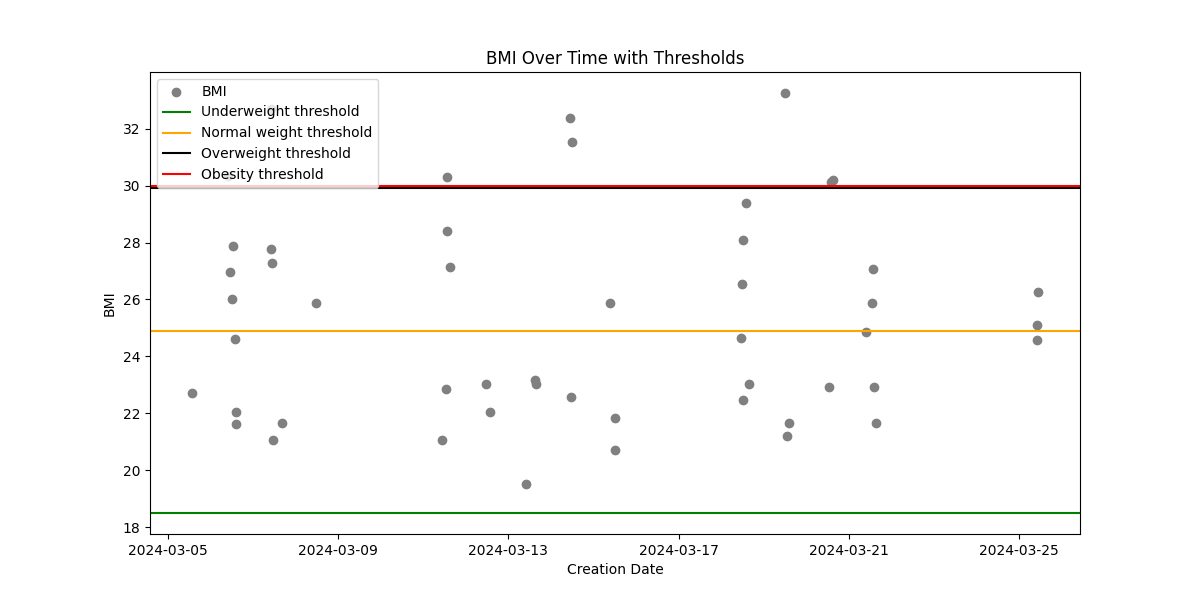
\includegraphics[width=1.0\linewidth]{Master Thesis/Plots/BMI.png}
\caption{Distribution of BMI values of all subjects}
\label{fig:distBMI}
\end{figure}
\FloatBarrier

To address the sex determination challenge, a general BMI formula was employed. The BMI values were calculated and general thresholds were plotted to categorize the subjects effectively. The plot illustrates the distribution of BMI values over time, showcasing various thresholds for underweight, normal weight, overweight, and obesity as defined by the World Health Organization (WHO).

As seen in the figure ~\ref{fig:distBMI}, none of the subjects is in the underweight category. A significant number of subjects have a BMI within the normal range. Some subjects exhibit a BMI over 25, indicating slight overweight, while a few have a BMI over 30, which is classified as unhealthy overweight according to WHO standards. This distribution provides valuable insights into the overall health status of the subjects, allowing for a better understanding of the population under study.

By integrating BMI calculations into the analysis, it becomes possible to gain a more comprehensive view of the subjects' health metrics, going beyond simple feature-based categorization. This approach underscores the importance of utilizing multiple health indicators to achieve more accurate and informative results. The use of BMI as an additional metric provides a clearer picture of the health and fitness levels of the subjects, which is crucial for making more informed conclusions and recommendations.

\section{Cross Entropy of the Study Dataset}

For getting a even better insight into our data, we calculated the cross entropy for the most important features of our work. Cross entropy is a key concept in information theory used to measure the difference between two probability distributions. When comparing two distributions, cross entropy quantifies the amount of additional information required to describe one distribution using another. This measurement is especially useful for analyzing how one set of values diverges from another, offering insights into their similarity or dissimilarity. By calculating cross entropy, we can better understand the distributional characteristics of different datasets, which is essential for various applications in statistics and data analysis.

For the feature heart rate, we obtained a cross entropy value of 0.98. This relatively low value indicates that the heart rate distributions between males and females are quite similar, as shown in the following plot:

\FloatBarrier
\begin{figure}[h!]
\centering
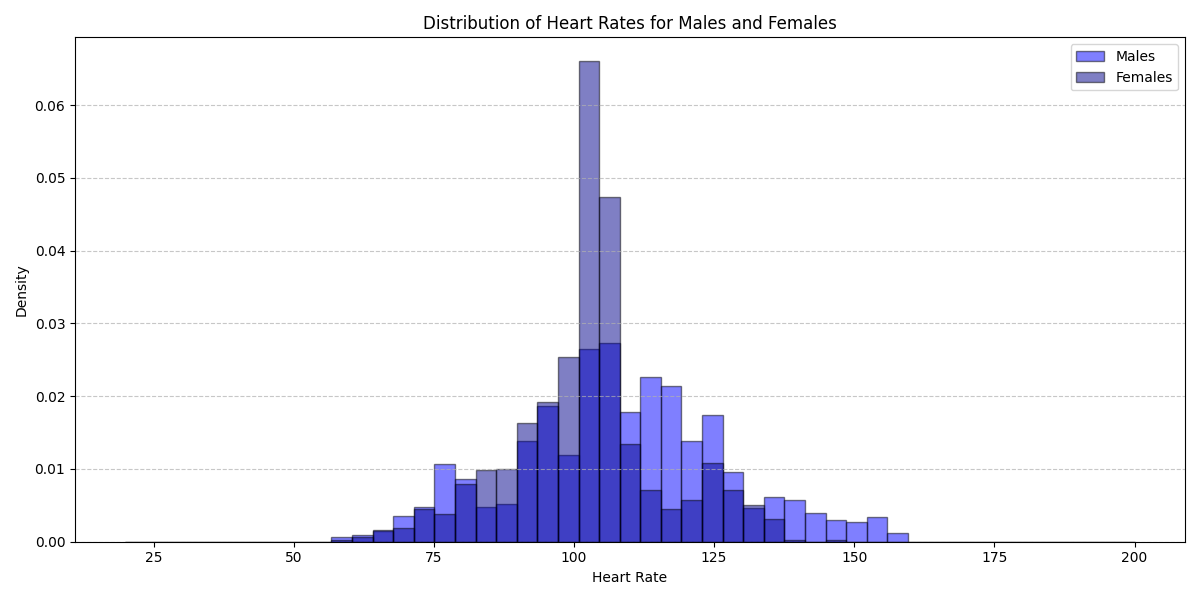
\includegraphics[width=1.0\linewidth]{Master Thesis/Plots/Dist_HeartRate_Males_Females.png}
\caption{Distribution of heart rates for males and females}
\label{fig:crossHeart}
\end{figure}
\FloatBarrier

In figure ~\ref{fig:crossHeart}, the distribution of heart rates for both male and female subjects is depicted. The plot shows that both distributions follow a similar pattern, with most heart rates clustering around 75 to 100 bpm. The peak of the male distribution is slightly higher than that of the female distribution, indicating a marginally higher heart rate in males. However, the overlap between the distributions suggests that heart rate behaviors are generally similar between sex.

The cross entropy between male and female active energy burned is 9.85, suggesting a significant difference in the distribution of active energy expenditure between the sex. The following plot illustrates these differences:

\FloatBarrier
\begin{figure}[h!]
\centering
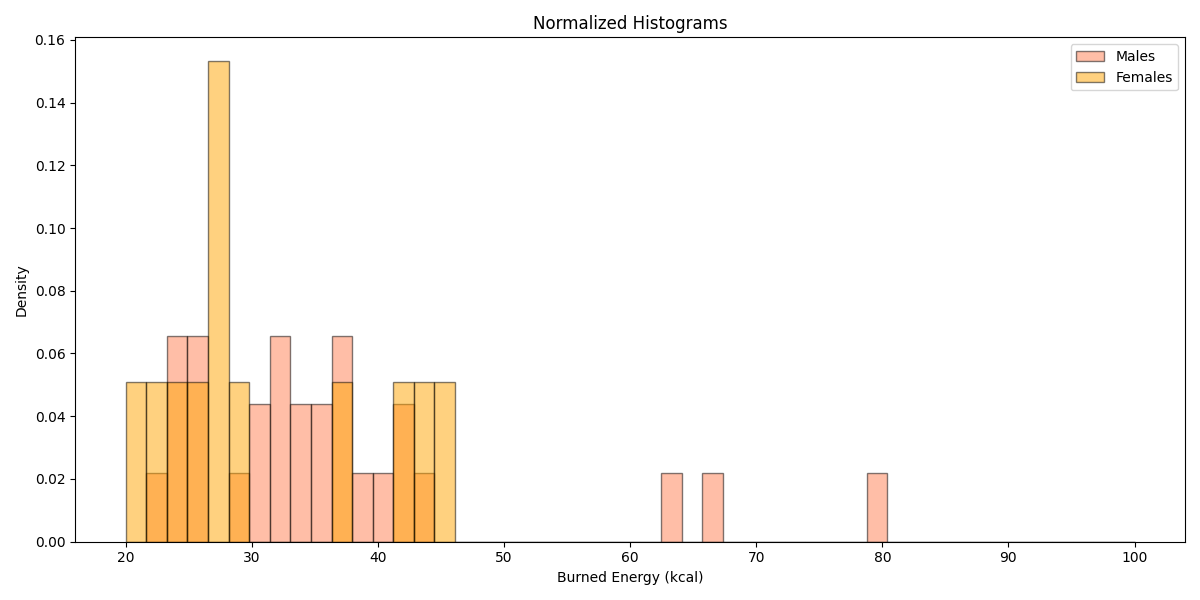
\includegraphics[width=1.0\linewidth]{Master Thesis/Plots/CrossEntro_ActiveEnergyBurned_all.png}
\caption{Distribution of active energy burned for males and females}
\label{fig:distActBurn}
\end{figure}
\FloatBarrier

Figure ~\ref{fig:distActBurn} illustrates the distribution of active energy burned for males and females. The plot reveals noticeable differences, with males generally burning more active energy compared to females. The male distribution shows a peak around 40 to 50 kcal, while the female distribution peaks around 20 to 30 kcal. This indicates that males tend to engage in more intense physical activities that burn higher amounts of energy.

For the basal energy burned, the cross entropy value is 19.49, indicating a considerable divergence between the distributions for males and females. This is depicted in the following plot:

\FloatBarrier
\begin{figure}[h!]
\centering
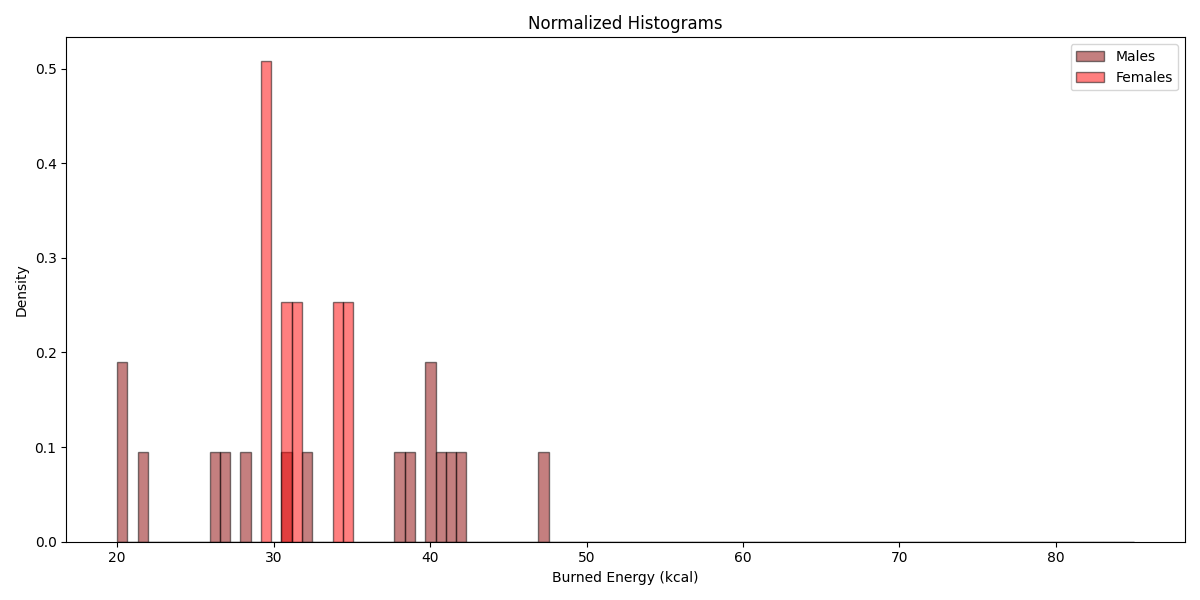
\includegraphics[width=1.0\linewidth]{Master Thesis/Plots/CrossEntro_BasalEnergyBurned_all.png}
\caption{Distribution of basal energy burned for males and females}
\label{fig:Distbasburn}
\end{figure}
\FloatBarrier

In figure ~\ref{fig:Distbasburn}, the distribution of basal energy burned during the recorded movement session is shown for both sex. The plot shows a clear divergence, with males generally burning more basal energy than females. The male distribution peaks around 1500 to 2000 kcal, while the female distribution peaks around 1000 to 1500 kcal. This significant difference reflects the higher basal metabolic rate in males, which is consistent with physiological differences between sex.

Regarding the walked distance, we achieved a cross entropy value of 8.46. This value suggests a moderate difference in the distribution of walked distances between males and females, as illustrated in the following plot:

\FloatBarrier
\begin{figure}[h!]
\centering
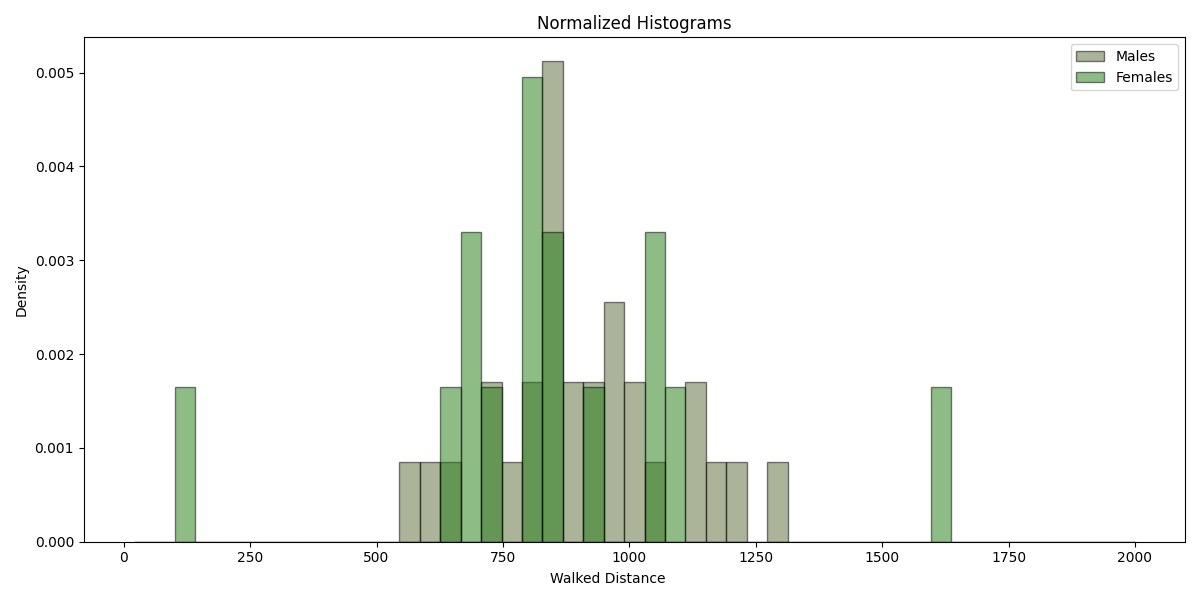
\includegraphics[width=1.0\linewidth]{Master Thesis/Plots/CrossEntro_Distance_all.jpeg}
\caption{Distribution of walked distances for males and females}
\label{fig:distWalkedRun}
\end{figure}
\FloatBarrier

Figure ~\ref{fig:distWalkedRun} displays the distribution of walked distances in meters for males and females. The plot shows that males tend to walk slightly longer distances than females. The male distribution has a peak around 1000 m, while the female distribution shows a peak around 750 m. However, the overall distribution is relatively similar between the two sex, indicating that walking distance is a more uniform activity across sex compared to energy expenditure metrics.

These cross entropy values provide valuable insights into the differences and similarities in health metrics between male and female subjects within the study dataset. Understanding these divergences helps to inform further analysis and applications in the field of health data analysis.

\newpage

We have now described the process of data extraction and preparation in detail. We have focused on the critical aspects of the study dataset. We described the methods used to convert XML files into CSV tables, the selection and merging of relevant data from different sources, and the specific criteria used to ensure the accuracy and completeness of the dataset. We also explained the rationale for selecting certain characteristics and metrics, such as heart rate values and BMI calculations, to provide a comprehensive basis for our analysis.
\chapter{Implementation and Results}
\label{cha:results}

In this chapter, we detail the implementation of various models and methods from both supervised and unsupervised learning to predict health metrics. We focus on their application, performance, and optimization. The analysis covers the used algorithms, the reasons for their selection and the achieved results. We want to highlight their predictive accuracy and reliability for health data. Additionally we want to predict a wide variety of features in this chapter, for example whether the test subject is sick or healthy.

\section{Supervised Learning Models}

In this section, we aim to evaluate the performance of supervised learning models on our dataset. The goal is to determine how well these models can predict health metrics based on the collected data before attempting to uncover correlations in relation to the 6MWT. We first prepared the dataset by cleaning and transforming the data, as previously described.

\subsection{Random Forest Models}

To begin our implementation of the methods, we chose to use a RF classifier due to its effectiveness in binary classification tasks. We then considered which classifications would be most meaningful for our analysis. This led to the idea of assessing risk levels among subjects based on their BMI. Consequently, we added a new column to the dataset that classifies subjects with a BMI value over 25 as at-risk. In this column, an entry of '0' indicates no risk, while an entry of '1' indicates a risk, but just in the implementation. Although BMI is not directly measurable by the Apple Watch Ultra, we aimed to see how well the watch's data could predict this risk factor. The features used for the input variable included age, weight, and height (none of which were measured by the Apple Watch Ultra) and step count. We wanted to predict whether a subject is exposed to a health risk or not. We achieved an accuracy of 0.94. The results are presented in the following table:

\begin{table}[H]
\centering
\begin{tabular}{lrrrr}
\toprule
{} & precision & recall & f1-score & support \\
\midrule
no risk & 0.92 & 1.00 & 0.96 & 11.00 \\
risk & 1.00 & 0.80 & 0.89 & 5.00 \\
macro avg & 0.96 & 0.90 & 0.92 & 16.00 \\
weighted avg & 0.94 & 0.94 & 0.94 & 16.00 \\
\bottomrule
\end{tabular}
\caption{RF classification for health risk with features age, weight, and height}
\label{table:sectryclass}
\end{table}

In the creation of the tables, we used the Python 'classification\_report' package. The reported averages include macro average, which averages the unweighted mean per label, and weighted average, which averages the support-weighted mean per label. By using these different types of averages, we can obtain a comprehensive view of the model's performance across all classes.

A closer look at these results in table ~\ref{table:firsttryclass} shows a recall value of 1.00 for class 'no risk', meaning the model identified 100$\%$ of all instances in this class correctly. For class 'risk', the recall value is 0.80, indicating that 80$\%$ of the instances were correctly identified. In general, a higher f1-score indicates better model performance. The f1-score for class 'no risk' is 0.96, indicating high precision and recall, whereas the f1-score for class 'risk' is 0.89, indicating good precision and fairly good recall.

The accuracy of 0.94 means that 94$\%$ of all predictions were correct. The macro average for precision, recall, and f1-score is the unweighted mean value for each class, suggesting the model performs well across both classes, with slightly better precision than recall. The weighted average accounts for the imbalance in support between the classes, with precision, recall, and f1-score all at 0.94, indicating high overall performance.

Next, the same model was implemented with adjusted features. This time, age (provided through the initial settings and shared Google table), the heart rate measured by the Apple Watch Ultra, which consists of the three values maximum heart rate, minimum heart rate and average heart rate, and step count were used as input features. The goal remained to predict the same risk factor as before and observe how the results compared. The outcomes were as follows with an accuracy of 0.75:

\begin{table}[H]
\centering
\begin{tabular}{lrrrr}
\toprule
{} & precision & recall & f1-score & support \\
\midrule
no risk & 0.89 & 0.73 & 0.80 & 11.00 \\
risk & 0.57 & 0.80 & 0.67 & 5.00 \\
macro avg & 0.73 & 0.76 & 0.73 & 16.00 \\
weighted avg & 0.79 & 0.75 & 0.76 & 16.00 \\
\bottomrule
\end{tabular}
\caption{RF classification for health risk with features maximum heart rate, minimum heart rate and average heart rate, and step count}
\label{table:firsttryclass}
\end{table}

The table above ~\ref{table:sectryclass} shows the performance metrics for the RF classifier. The following confusion matrix figure ~\ref{fig:ConfusionMatrixrisk1} visualizes these results:

\FloatBarrier
\begin{figure}[h!]
\centering
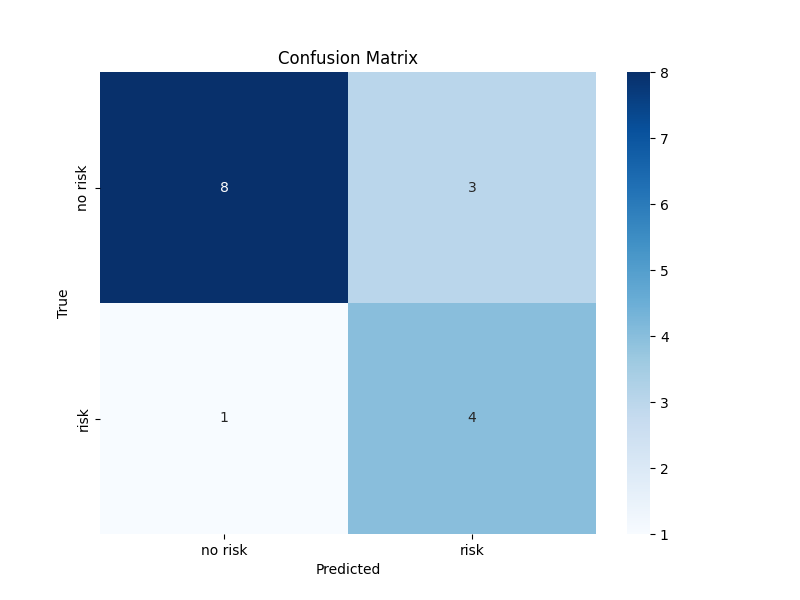
\includegraphics[width=1.0\linewidth]{Master Thesis/Plots/Confusion Matrix risk 1.png}
\caption{Confusion matrix of health risk classification with RF and features maximum heart rate, minimum heart rate and average heart rate, and step count}
\label{fig:ConfusionMatrixrisk1}
\end{figure}
\FloatBarrier

This confusion matrix indicates that the model correctly predicted the 'no risk' class in most cases, but made some errors in predicting the 'risk' class. The precision and recall for both classes reflect this distribution, with higher precision for 'no risk' compared to 'risk'.

The results in general indicate that the model's performance declined compared to the previous version, suggesting that the model places greater importance on non-Apple Watch Ultra data. This was evident when the feature 'age' was removed from the training set, yet the results remained unchanged, indicating that age does not significantly impact this prediction. The decline in performance when incorporating features measured explicitly by the Apple Watch Ultra implies that modifications are necessary to improve the model's effectiveness in utilizing Apple Watch Ultra data for making accurate predictions. This is crucial as our goal is to evaluate how well the data from the Apple Watch Ultra can be used for such predictions.

\subsubsection*{Optimizing the Results of the Random Forest}

To further enhance the results, we utilized the Gradient Boosting Classifier. For this model, we incorporated three heart rate measures (minimum, maximum, and average heart rate over each 6-minute interval of a subject) along with the subject's age, which is not measured by the Apple Watch Ultra. Our aim was to predict the risk by classifying individuals with a BMI over 25 as at-risk. The results using the RF classifier were as following with an accuracy of 0.50:

\begin{table}[H]
\centering
\begin{tabular}{lrrrr}
\toprule
{} & precision & recall & f1-score & support \\
\midrule
no risk & 0.50 & 0.75 & 0.60 & 8.0 \\
risk & 0.50 & 0.25 & 0.33 & 8.0 \\
macro avg & 0.50 & 0.50 & 0.47 & 16.0 \\
weighted avg & 0.50 & 0.50 & 0.47 & 16.0 \\
\bottomrule
\end{tabular}
\caption{RF classification for health risk with features heart rates (minimum, maximum, and average heart rate over each 6-minute interval of a subject) along with the age}
\label{table:thirdtryclass}
\end{table}
The table above ~\ref{table:thirdtryclass} shows the performance metrics for the RF classifier with a lower accuracy. The following confusion matrix visualizes these results:
\FloatBarrier
\begin{figure}[h!]
\centering
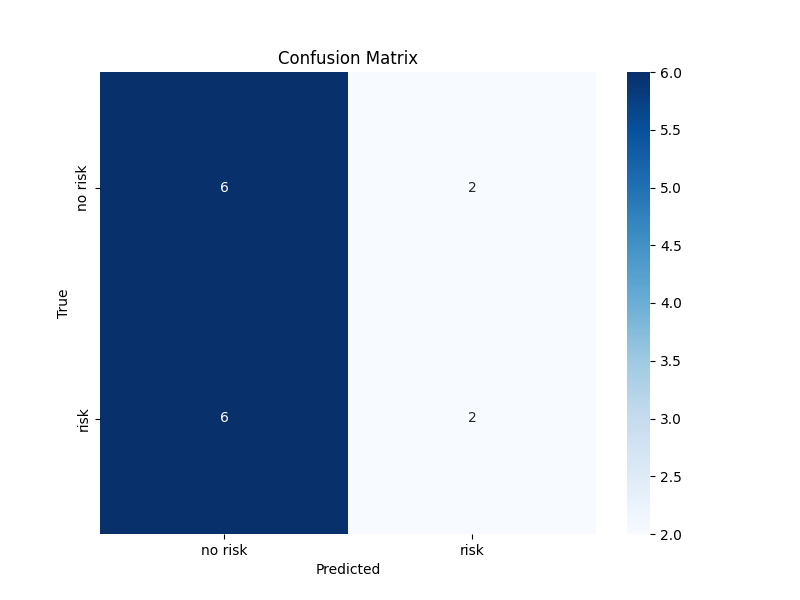
\includegraphics[width=1.0\linewidth]{Master Thesis/Plots/Confusion Matrix risk 2.png}
\caption{Confusion matrix of health risk classification with RF and features heart rates (minimum, maximum, and average heart rate over each 6-minute interval of a subject) along with the age}
\label{fig:ConfusionMatrixrisk2}
\end{figure}
\FloatBarrier

This confusion matrix figure ~\ref{fig:ConfusionMatrixrisk2} demonstrates that the model performs worse in predicting the 'risk' class, as it misclassifies the same number of 'risk' instances as 'no risk' as it correctly classifies. This is confirmed by the lower precision and recall values for the 'risk' class.

The table ~\ref{table:thirdtryclass} shows the performance metrics for the RF Classifier. The precision for both classes is 0.50, indicating that half of the predictions for each class were correct. The recall for class 'no risk' is higher at 0.75, meaning 75\% of the actual class 'no risk' instances were correctly identified, while only 25\% of class 'risk' instances were correctly identified. This imbalance suggests the model is better at identifying non-risk subjects than at identifying at-risk subjects. The f1-scores are 0.60 for class 'no risk' and 0.33 for class 'risk', showing a substantial drop in performance for class 'risk'. The overall accuracy is 50\%, which means the model's predictions are essentially no better than random guessing. The macro average and weighted average f1-scores reflect this poor performance, both at approximately 0.47. These results suggest that the model, in its current form, is not suitable for predicting risk based on the given features.

In contrast, using the gradient boosting classifier, we where able to achieve an accuracy of 0.81 and the following results:

\begin{table}[H]
\centering
\begin{tabular}{lrrrr}
\toprule
{} & precision & recall & f1-score & support \\
\midrule
no risk & 0.78 & 0.88 & 0.82 & 8.0 \\
risk & 0.86 & 0.75 & 0.80 & 8.0 \\
macro avg & 0.82 & 0.81 & 0.82 & 16.0 \\
weighted avg & 0.82 & 0.81 & 0.82 & 16.0 \\
\bottomrule
\end{tabular}
\caption{Gradient boosting classification with features heart rates (minimum, maximum, and average heart rate over each 6-minute interval of a subject) along with the age}
\label{table:boostnr1}
\end{table}

The table ~\ref{table:boostnr1} shows the performance metrics for the gradient boosting classifier. The precision for class 'no risk' is 0.78 and for class 'risk' is 0.86, indicating that the model correctly identifies a high proportion of both non-risk and at-risk subjects. The recall for class 'no risk' is 0.88, meaning 88\% of the actual non-risk instances were correctly identified, while the recall for class 'risk' is 0.75, indicating that 75\% of the actual at-risk instances were correctly identified. The f1-scores are 0.82 for class 'no risk' and 0.80 for class 'risk', reflecting a balanced performance in precision and recall for both classes. The overall accuracy is 81\%, showing a significant improvement compared to the previous model. The macro average and weighted average f1-scores are both at 0.82, demonstrating consistent performance across the dataset. These results suggest that the Gradient Boosting Classifier is more reliable for predicting risk based on the given features.

The RF classifier provided a good initial model for predicting risk among subjects, with promising accuracy and performance metrics. Further optimization using the Gradient Boosting Classifier significantly improved the results, making it a more reliable model for risk prediction in this context.

\subsection{Subject or Patient Classification with Random Forest}

In this subsection, we focus on classifying individuals as either patients (those with health issues) or subjects (healthy individuals). Additionally, we continue to use the previously introduced risk category, for individuals with a BMI over 25, suggesting a higher likelihood of developing health issues. This categorization aims to achieve an even clearer distinction, recognizing that overweight individuals are at increased risk of long-term health problems. The features used in our models include age (not measured by the Apple Watch Ultra) and distance (measured by the Apple Watch Ultra).

Using this set of features (age and distance), the RF model achieved an accuracy of 0.94. Detailed results are shown below:

\FloatBarrier
\begin{table}[H]
\centering
\begin{tabular}{lrrrr}
\toprule
{} & precision & recall & f1-score & support \\
\midrule
patient & 0.91 & 1.00 & 0.95 & 10.00 \\
subject & 1.00 & 0.83 & 0.91 & 6.00 \\
macro avg & 0.95 & 0.92 & 0.93 & 16.00 \\
weighted avg & 0.94 & 0.94 & 0.94 & 16.00 \\
\bottomrule
\end{tabular}
\caption{RF classification with features age and distance}
\label{table:RFageDistance}
\end{table}
\FloatBarrier

The RF model using age and distance features shows excellent performance with an overall accuracy of 0.94. For the 'patient' category, the precision is 0.91, indicating that 91\% of those classified as patients were indeed patients. The recall for this category is 1.00, meaning all actual patients were correctly identified by the model. The f1-score for patients is 0.95, reflecting a balance between precision and recall.

For the 'subject' category, the precision is 1.00, indicating perfect identification of all healthy individuals classified as subjects. The recall for subjects is 0.83, meaning 83\% of actual subjects were correctly identified, with some misclassified as patients. The f1-score for subjects is 0.91.

The macro average f1-score, which is the unweighted mean of the f1-scores for all classes, is 0.93. This suggests that the model performs well across both categories. The weighted average f1-score, which accounts for the number of instances in each class, is 0.94, indicating strong overall model performance.

Using the second set of features (age and heart rate), which includes age (not measured by the Apple Watch Ultra) and heart rate (measured by the Apple Watch Ultra), the model also achieved an accuracy of 0.94:

\FloatBarrier
\begin{table}[H]
\centering
\begin{tabular}{lrrrr}
\toprule
{} & precision & recall & f1-score & support \\
\midrule
patient & 0.91 & 1.00 & 0.95 & 10.00 \\
subject & 1.00 & 0.83 & 0.91 & 6.00 \\
macro avg & 0.95 & 0.92 & 0.93 & 16.00 \\
weighted avg & 0.94 & 0.94 & 0.94 & 16.00 \\
\bottomrule
\end{tabular}
\caption{RF classification with features age and heart rate}
\label{table:RFageHeartrate}
\end{table}
\FloatBarrier

The RF model using age and heart rate features demonstrated high accuracy and effective classification. Precision and recall values were strong for both patient and subject categories, indicating the model's reliability with these features. Specifically, the recall for patients is 1.00, meaning all patient instances were correctly identified. The precision for subjects is 1.00, showing no false positives in identifying subjects.

Using the third set of features (distance and heart rate), both measured by the Apple Watch Ultra, the accuracy dropped to 0.63:

\FloatBarrier
\begin{table}[H]
\centering
\begin{tabular}{lrrrr}
\toprule
{} & precision & recall & f1-score & support \\
\midrule
patient & 0.62 & 1.00 & 0.77 & 10.00 \\
subject & 0.00 & 0.00 & 0.00 & 6.00 \\
macro avg & 0.31 & 0.50 & 0.38 & 16.00 \\
weighted avg & 0.39 & 0.62 & 0.48 & 16.00 \\
\bottomrule
\end{tabular}
\caption{RF classification with features distance and heart rate}
\label{table:RFdistHeartrate}
\end{table}
\FloatBarrier

The model's performance significantly decreased with an accuracy of 0.62 when using only distance and heart rate features. This suggests that these features alone are insufficient for accurate classification. The recall for patients is still high at 1.00, but the precision for subjects is 0.00, indicating the model struggled to correctly classify subjects based on these features alone. This suggests that the model is very dependent on information that the Apple Watch Ultra does not measure and that the results with only Apple Watch Ultra data are simply not meaningful enough.

Incorporating all three features (distance, heart rate, and age), where age is not measured by the Apple Watch Ultra, the model achieved an accuracy of 0.94:

\FloatBarrier
\begin{table}[H]
\centering
\begin{tabular}{lrrrr}
\toprule
{} & precision & recall & f1-score & support \\
\midrule
patient & 0.91 & 1.00 & 0.95 & 10.00 \\
subject & 1.00 & 0.83 & 0.91 & 6.00 \\
macro avg & 0.95 & 0.92 & 0.93 & 16.00 \\
weighted avg & 0.94 & 0.94 & 0.94 & 16.00 \\
\bottomrule
\end{tabular}
\caption{RF classification with features age, heart rate and distance}
\label{table:RFageHeartrateDist}
\end{table}
\FloatBarrier

Including all three features restored the accuracy to 0.94, demonstrating the significance of a comprehensive feature set. The high precision and recall values across both patient and subject categories reinforce the model's reliability and effectiveness. This shows the importance of including multiple relevant features to enhance classification performance, indicating that the model can effectively identify at-risk patients when a broader range of data is used. However, this also leads to the assumption that the model primarily takes into account the age of the test subjects in order to categorize them as sick or healthy.

In summary, the RF model showed consistent high accuracy when age was included as a feature, indicating its crucial role in risk prediction. Conversely, using only the features directly measured by the Apple Watch Ultra (distance and heart rate) resulted in poorer performance. This suggests that while the Apple Watch Ultra provides valuable data, incorporating additional features such as age is essential for improving model accuracy and reliability in predicting health risks.

\subsection{Regression Models}

After using RF, we turned to regression analysis, believing it could help us not only classify data but also predict continuous values accurately. In this section, we explore how close our predictions are to actual values using the RMSE.

We started with linear regression to predict the age of subjects— a feature not measured by the Apple Watch Ultra—using data collected by the watch. Initially, we used height and weight, both not measured by the watch, to establish a baseline model.

Our first linear regression model predicted age with an RMSE of 21.92, showing the average deviation of predicted ages from actual ages. By starting with these features, we set a baseline to evaluate the impact of incorporating Apple Watch Ultra data in improving our predictions. This approach helped us understand which features best predict various health metrics, enhancing our knowledge of the watch's capabilities in health monitoring.

\FloatBarrier
\begin{figure}[h!]
\centering
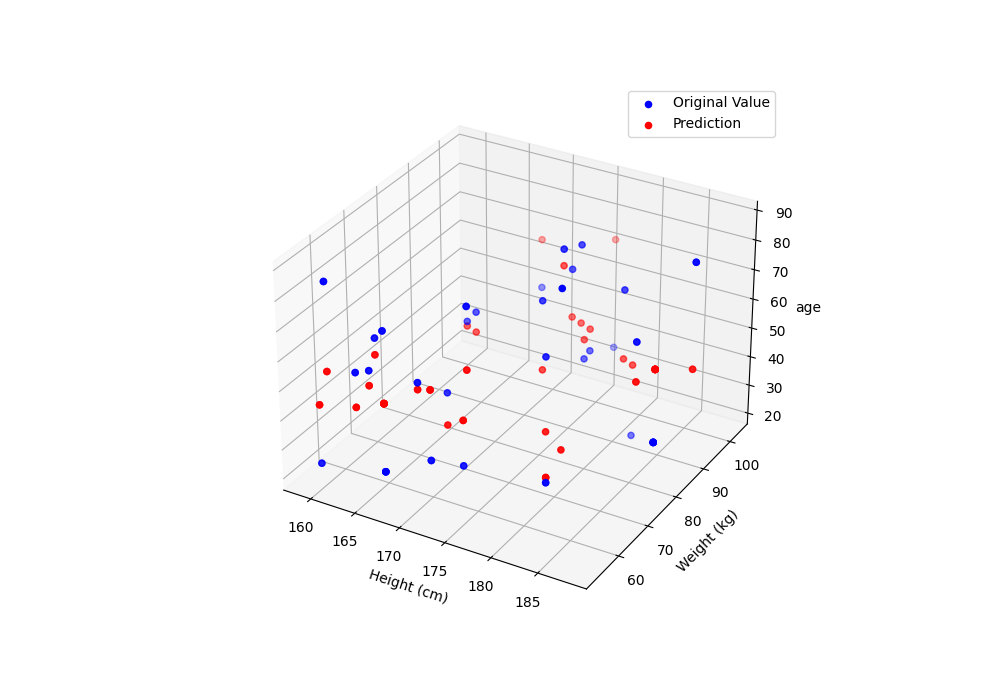
\includegraphics[width=0.9\textwidth]{Master Thesis/Plots/prediction3.png}
\caption{Age prediction with regression based on the features height and weight}
\label{figure:regwithheightweight}
\end{figure}
\FloatBarrier

Figure ~\ref{figure:regwithheightweight} shows a 3D scatter plot comparing actual ages (blue dots) to predicted ages (red dots) based on height and weight. The X-axis represents height in centimeters, the Y-axis shows weight in kilograms, and the Z-axis displays age in years. The closer the red dots are to the blue dots, the more accurate the age predictions by the linear regression model. This plot shows, that the predicted age and original age are quite far apart.

To improve prediction accuracy, we made another attempt with the same linear regression model but with different features. This time, we used leg length, a manually measured feature, and the walked distance, which was measured by the Apple Watch Ultra. Again, we aimed to predict age. This model achieved an RMSE value of 20.76, showing a slight improvement, but the result was still not very accurate.

\FloatBarrier
\begin{figure}[h!]
\centering
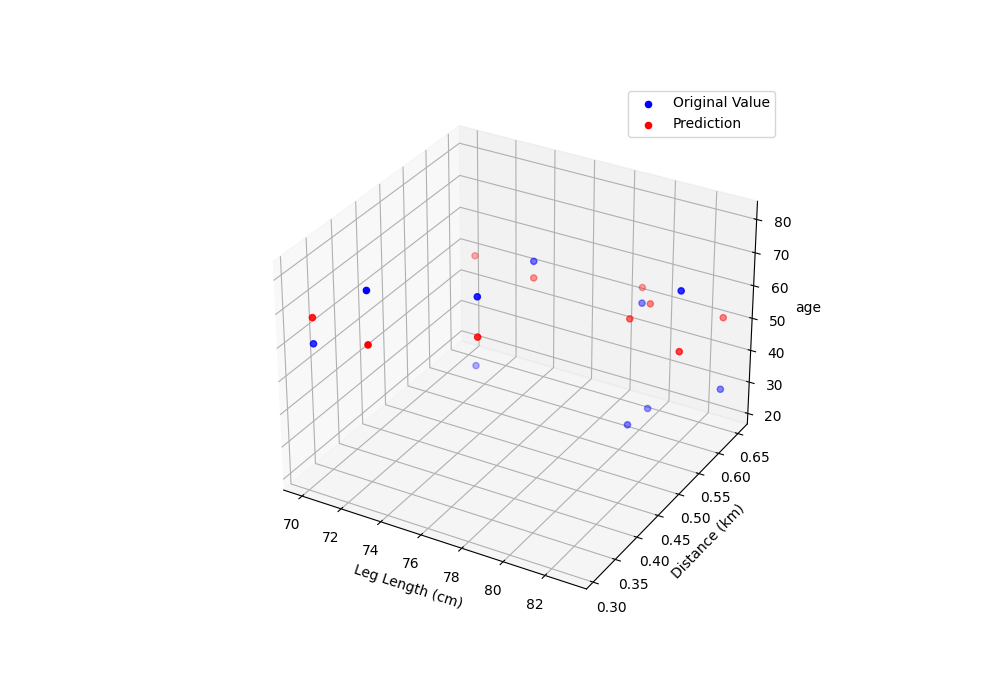
\includegraphics[width=0.9\textwidth]{Master Thesis/Plots/prediction2.png}
\caption{Age prediction with regression based on the leg length and distance}
\label{figure:regwithleglengthdistance}
\end{figure}
\FloatBarrier

Figure ~\ref{figure:regwithleglengthdistance} shows again, that the points are quite far apart from each other, what shows us some potential for optimizing the model or change the features to achieve better results.

While the second model performed better, the high RMSE values indicate that predicting age based solely on these features is challenging, with the predictions being off by over 20 years on average.

\subsubsection*{Expanding the Dataset for Better Predictions}
Recognizing the limitations of predicting age from height and weight alone, we expanded the dataset by including additional features such as heart rates and BMI. This approach aimed to develop more sophisticated models to predict health metrics.

We first attempted to enhance the age prediction model by adding maximum and minimum heart rates, as well as leg length. However, the results were still not very accurate. Believing that regression was still the right tool for such predictions, we next focused on predicting BMI instead of age. By using the feature heart rate (just the minimum value during one interval), we achieved an RMSE of 2.64, which was promising given the typical BMI range of 15 to 40. Further refinements, including using weighted regression with more heart rate data, will be explored later in this study.

\FloatBarrier
\begin{figure}[h!]
\centering
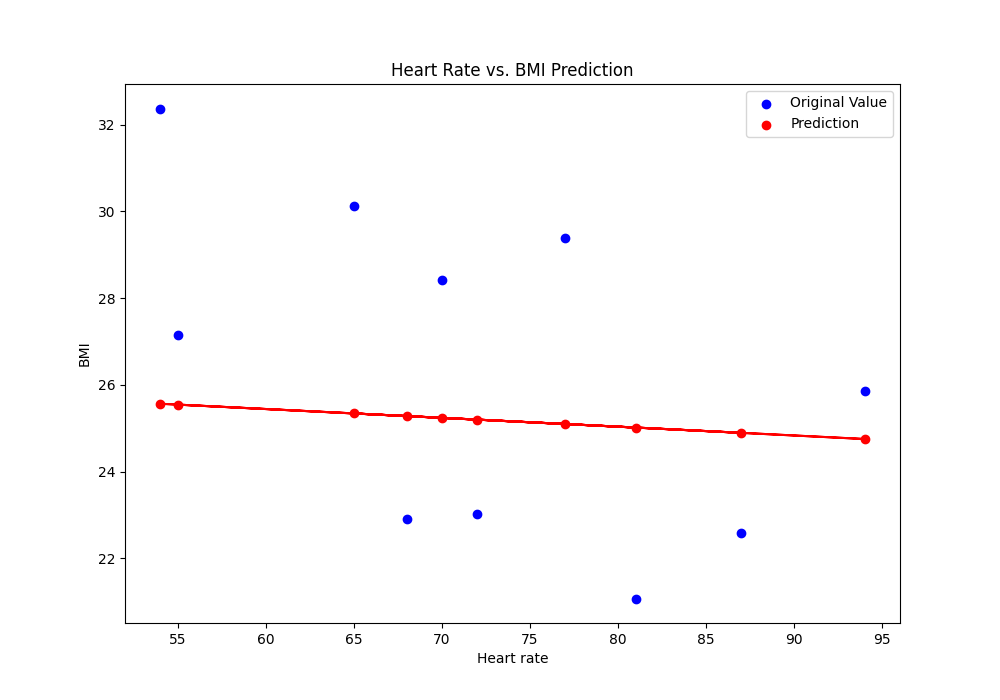
\includegraphics[width=0.6\textwidth]{Master Thesis/Plots/prediction_BMI.png}
\caption{BMI prediction with regression based on heart rate feature}
\label{figure:regwithheartrate}
\end{figure}
\FloatBarrier

The image, labeled as figure ~\ref{figure:regwithheartrate}, is a 2D scatter plot showing the original and predicted BMI values based solely on heart rates. The X-axis represents heart rate, and the Y-axis represents BMI. Red points indicate the original BMI values, while blue points represent the predictions made by the model. The plot shows that the predicted BMI values are randomly distributed around a narrow range, indicating that the model's predictions are not reliable and do not capture the true variability in BMI. The resulting RMSE value was high, suggesting significant prediction errors and demonstrating that heart rates alone are not sufficient to predict BMI accurately.

After initially using only one feature to predict BMI, we decided to incorporate maximum and minimum heart rates along with weight (not measured by the Apple Watch Ultra) as features to improve the prediction. By adding weight as a feature along with heart rates, we achieved a significantly lower RMSE of 1.57. The plot below demonstrates the improved accuracy:

\FloatBarrier
\begin{figure}[h!]
\centering
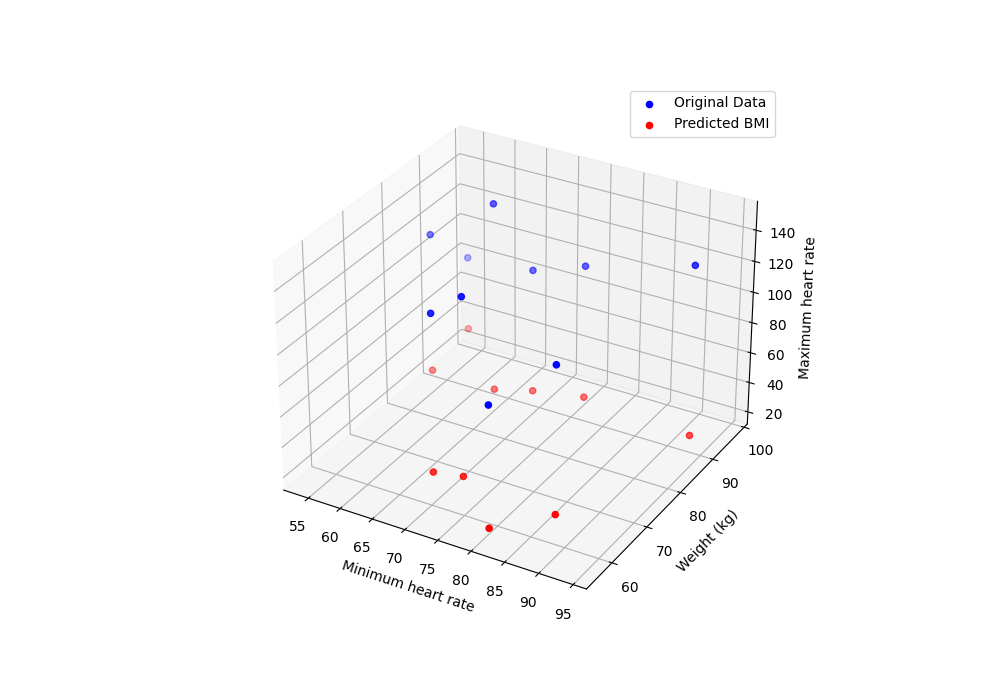
\includegraphics[width=0.9\textwidth]{Master Thesis/Plots/bmi_prediction.png}
\caption{BMI prediction with regression based on features weight and heart rate}
\label{figure:regwithheartrateweight}
\end{figure}
\FloatBarrier

The image, labeled as figure ~\ref{figure:regwithheartrateweight}, is a 3D scatter plot showing the original and predicted BMI values based on both weight and heart rates. The X-axis represents weight (kg), the Y-axis represents heart rate, and the Z-axis represents BMI. Red points indicate the original BMI values, while blue points represent the predictions made by the model. This plot shows a much closer alignment between the original and predicted BMI values, indicating a significant improvement in prediction accuracy. The model achieved a notably lower RMSE value of 1.57, reflecting a substantial reduction in prediction error compared to the previous model.

Although this result is promising, it is important to note that weight is innately included as part of the BMI calculation, making it easier for the model to accurately predict BMI.

With the restructured dataset, included maximum and minimum heart rates, weight, and age as features, we wanted to do another prediction. With these features, we aimed to predict the heart rate using a linear regression model before returning to the subject or patient classification topic using regression.

Using this data, we applied the same linear regression model to predict the actual heart rate based on the weight and age of the subjects. The model achieved an RMSE value of 17.01.

\FloatBarrier
\begin{figure}[h!]
\centering
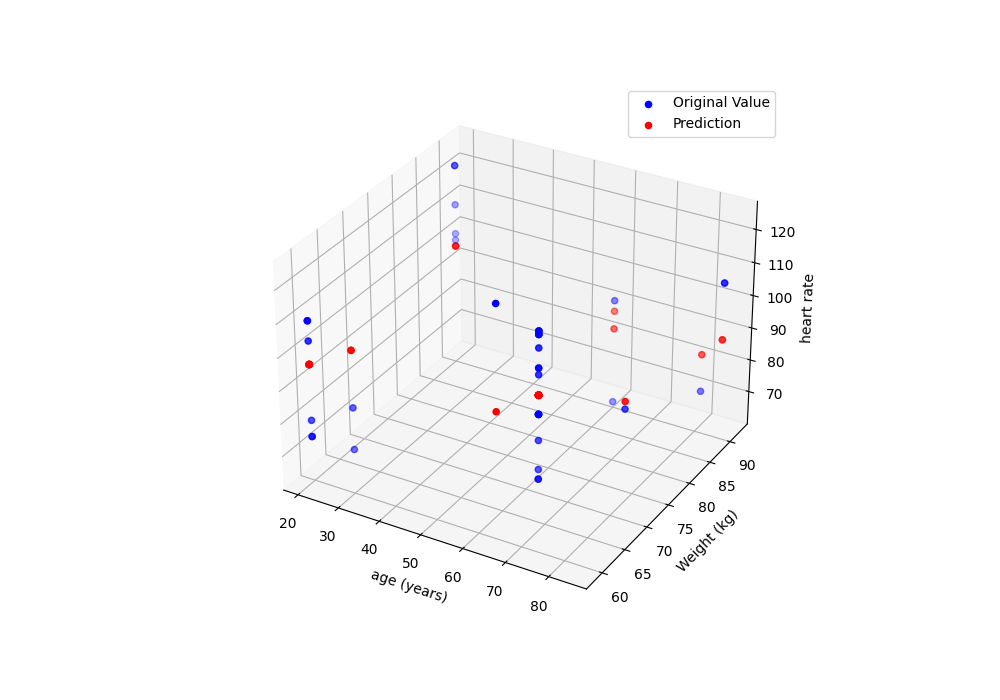
\includegraphics[width=0.9\textwidth]{Master Thesis/Plots/heart-rate_prediction.png}
\caption{Heart rate prediction with regression based on features weight and age}
\label{figure:HRregwithweightage}
\end{figure}
\FloatBarrier

Figure ~\ref{figure:HRregwithweightage} demonstrates a reasonably close alignment between the original and predicted heart rate values, indicating a moderate level of prediction accuracy. The model achieved a RMSE value of 17.01, reflecting the average deviation of the predicted values from the actual values. This RMSE value suggests that while the model's predictions are not perfect, they are within an acceptable range for many applications.

The scatter plot highlights that the model can capture the general trend of how heart rate varies with weight and age, but there are still some discrepancies. These discrepancies could be due to various factors, including the limited number of features used in the model and the inherent variability in heart rate that may be influenced by factors not included in the dataset.

\subsection{Subject or Patient Classification with Logistic Regression}

We used the same dataset from above to evaluate the effectiveness of logistic regression in classifying individuals as either 'patient' or 'subject', based on the risk of developing health issues due to being overweight (BMI over 25) or already being diseased.

Using linear regression, the RMSE was 0.26. Logistic regression yielded to the following results:

\FloatBarrier
\begin{table}[H]
\centering
\begin{tabular}{lcccc}
\toprule
& precision & recall & f1-Score & support \\
\midrule
patient & 0.91 & 1.00 & 0.95 & 10.0 \\
subject & 1.00 & 0.83 & 0.91 & 6.0 \\
macro avg & 0.95 & 0.92 & 0.93 & 16.0 \\
weighted avg & 0.94 & 0.94 & 0.94 & 16.0 \\
\bottomrule
\end{tabular}
\caption{Subject or patient classification with logistic regression based on BMI, heart rate and age}
\label{table:logregpatsubj}
\end{table}
\FloatBarrier

The results from the logistic regression model in table ~\ref{table:logregpatsubj} show a high overall accuracy of 0.94. For the 'patient' category, precision is 0.91, recall is 1.00, and the f1-score is 0.95, indicating that the model correctly identifies all patients but slightly overestimates their count. For the 'subject' category, precision is perfect at 1.00, recall is 0.83, and the f1-score is 0.91, showing that while all identified subjects are correct, some subjects are missed by the model.

The macro average scores, which are the unweighted mean of precision, recall, and f1-score, are also high (0.95, 0.92, and 0.93 respectively), indicating balanced performance across both categories. The weighted average, which accounts for the number of instances in each class, confirms the model's reliability with all metrics at 0.94.

Additionally, the following plots illustrate the predictions made by the logistic regression model and provide an overview of the results:

\FloatBarrier
\begin{figure}[h!]
\centering
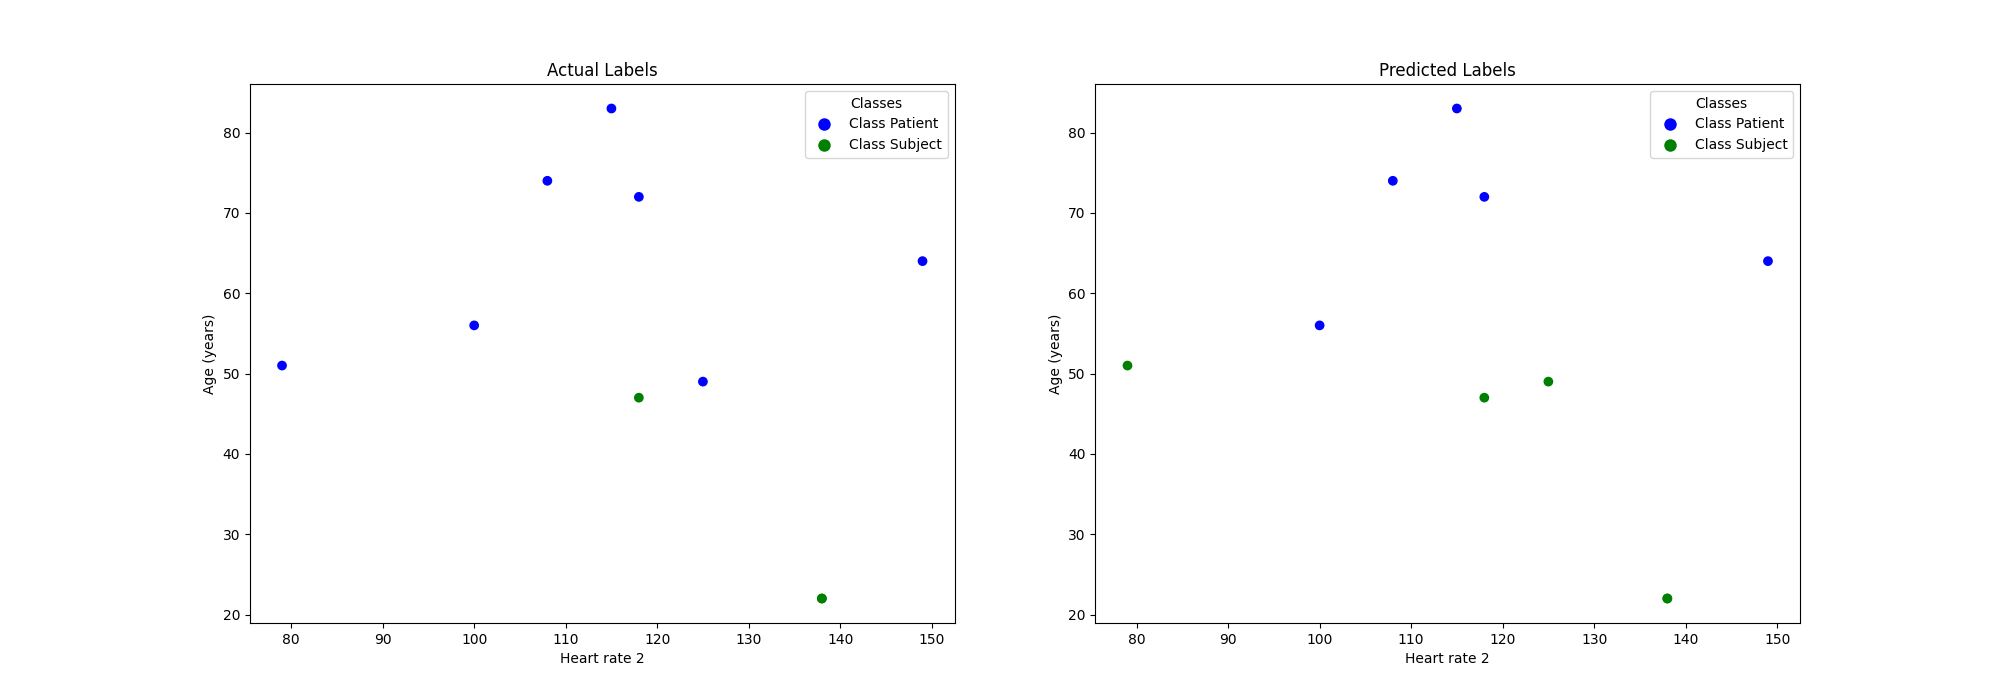
\includegraphics[width=1.1\textwidth]{Master Thesis/Plots/prediction_subjectpatient.png}
\caption{Subject or patient classification with logistic regression based on maximal heart rate and age}
\label{figure:logregwithheartrateage}
\end{figure}
\FloatBarrier

\FloatBarrier
\begin{figure}[h!]
\centering
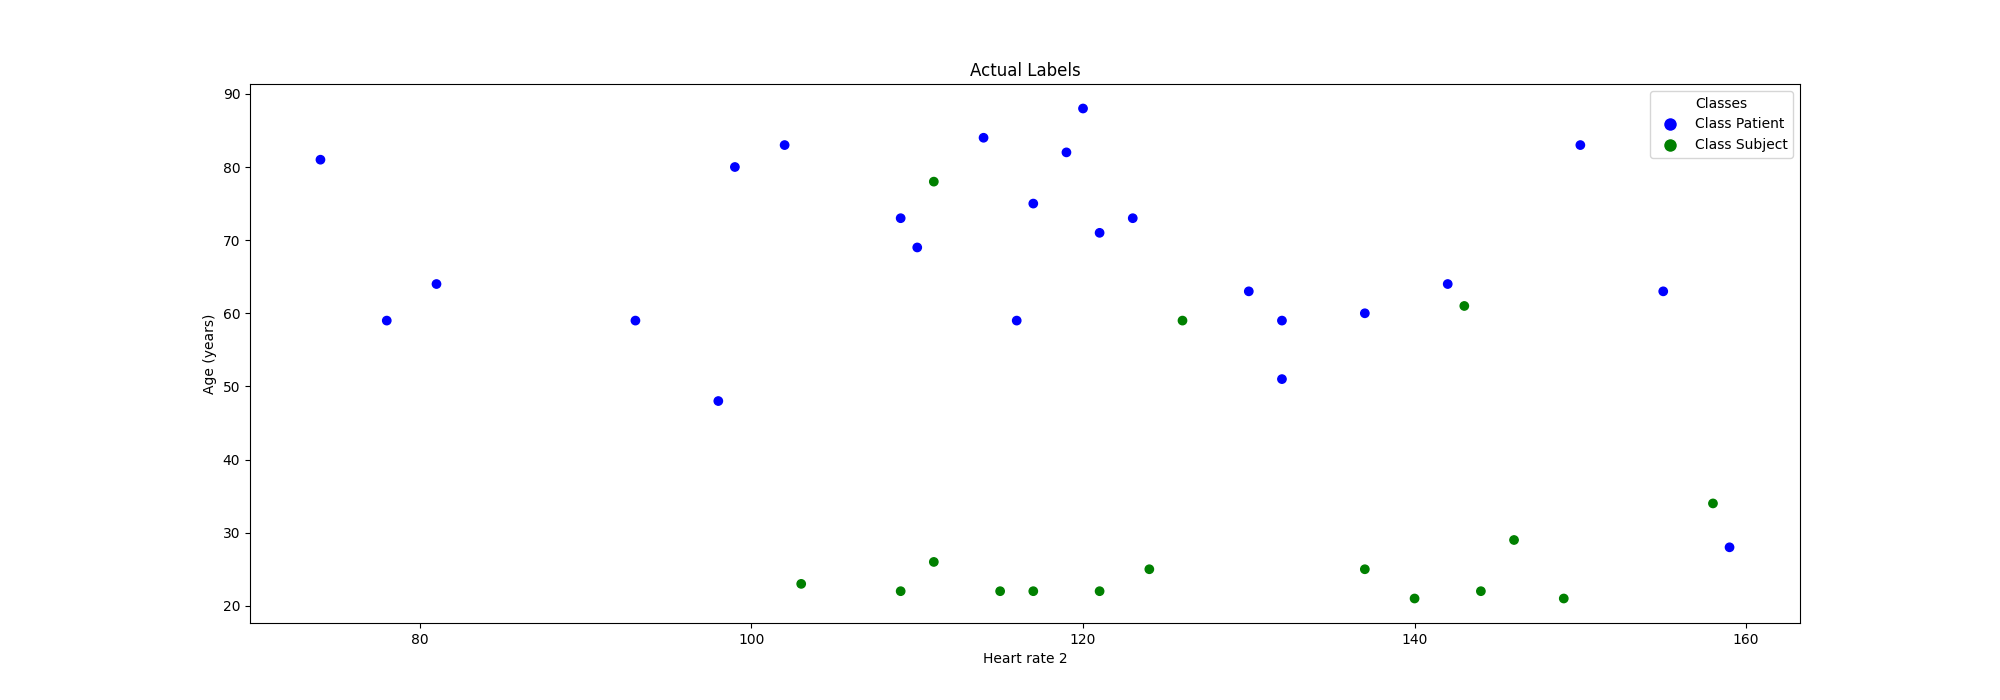
\includegraphics[width=0.9\textwidth]{Master Thesis/Plots/dataset_overview.png}
\caption{Subject or patient classification with logistic regression based on maximal heart rate and age all data}
\label{figure:logregwithheartrateageall}
\end{figure}
\FloatBarrier

The first two plots in figure ~\ref{figure:logregwithheartrateage} display the actual and predicted labels of 'subject/patient' status based on age and heart rate. The plot on the left shows the actual labels, where blue dots represent subjects and green dots represent patients. The plot on the right shows the predicted labels by the logistic regression model, similarly colored. The alignment of blue and green dots between the two plots indicates the model's accuracy in predicting the correct category.

Figure ~\ref{figure:logregwithheartrateageall} provides a comprehensive overview of the dataset, showing the distribution of subjects and patients based on age and heart rate. Each dot represents an individual, with blue dots indicating subjects and green dots indicating patients. This visualization helps in understanding the spread and clustering of the data points, as well as the relationship between age, heart rate and health status.

\subsection{Neural Networks}

In the methodology chapter ~\ref{cha:methods}, we introduced neural networks and aimed to test their suitability for this dataset. We considered various combinations of features to evaluate the deep learning models, which aimed to predict physiological measurements based on age and exercise behavior. Specifically, the models focused on predicting heart rate from age and walked distance. Additionally predicting walked distance from age and heart rate. And finally predicting age from heart rate and walked distance:

\FloatBarrier
\begin{table}[htbp]
\centering
\begin{tabular}{@{}lcc@{}}
\toprule
\textbf{model description} & \textbf{MSE} & \textbf{interpretation} \\ \midrule
heart rate prediction (age, distance) & 1.10 & moderate error \\
distance prediction (age, heart rate) & \textbf{0.59} & low error \\
age prediction (heart rate, distance) & 0.60 & low error \\ 
\bottomrule
\end{tabular}
\caption{Performance of deep learning models measured in MSE for different features}
\end{table}
\FloatBarrier

The model predicting heart rate based on age and distance achieved a MSE of 1.10, indicating a moderate level of error. This suggests that while age and distance have some predictive power, additional factors likely influence heart rate that are not captured by these two variables alone.

Predicting distance walked based on age and heart rate resulted in a low MSE of 0.59. This low error indicates a strong relationship between these variables, implying that the model can accurately predict distance traveled with the given inputs. This suggests good predictive accuracy and a strong link between physical activity, age, and heart rate.

The model predicting age based on heart rate and distance traveled achieved an MSE of 0.60. The low error suggests that these two features provide valuable information about the biological age of an individual, which could highlight discrepancies between biological and chronological age based on fitness data.

We then applied a slightly modified version of the same deep learning model, focusing on visualizing the results and calculating accuracy instead of the MSE. 

\FloatBarrier
\begin{figure}[h!]
\centering
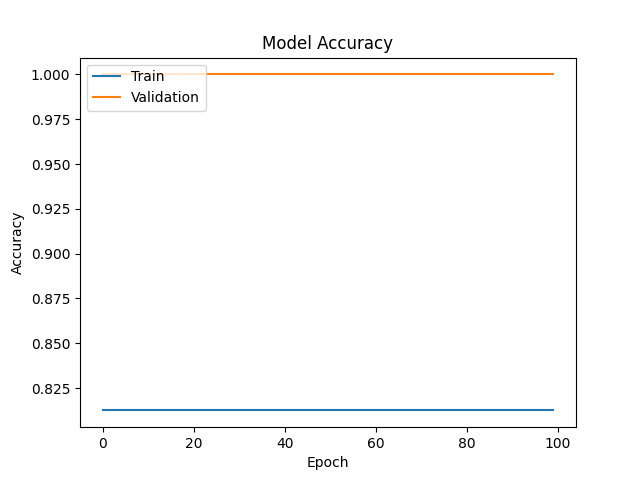
\includegraphics[width=0.8\textwidth]{Master Thesis/Plots/deepLearningModel_age+heartRate1.png}
\caption{Accuracy of deep learning model}
\label{figure:modelaccNN}
\end{figure}
\FloatBarrier

\FloatBarrier
\begin{figure}[h!]
\centering
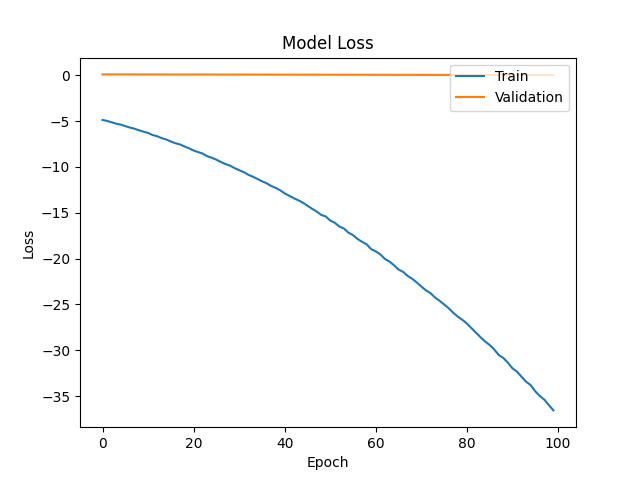
\includegraphics[width=0.8\textwidth]{Master Thesis/Plots/deepLearningModel_age+heartRate2.png}
\caption{Loss of deep learning model}
\label{figure:modellossNN}
\end{figure}
\FloatBarrier

Using the features of age and heart rate, the model achieved an accuracy of 81.25\%. This means that the model correctly predicted or classified 81.25$\%$ of the test dataset, indicating a strong performance. 

Figure ~\ref{figure:modelaccNN} shows the model accuracy, with the X-axis representing the number of epochs and the Y-axis representing the accuracy. The blue line indicates the training accuracy, and the orange line indicates the validation accuracy. The plot reveals that the training accuracy remains constant and low throughout the epochs, suggesting that the model is not improving its performance on the training data. In contrast, the validation accuracy is constant and perfect (1.0) from the beginning. This unusual behavior may indicate a potential issue in the training process.

Figure ~\ref{figure:modellossNN} displays the model loss, with the X-axis denoting the number of epochs and the Y-axis denoting the loss value. The blue line represents the training loss, and the orange line represents the validation loss. The training loss consistently decreases over the epochs, indicating that the model is learning and fitting the training data progressively better. However, the validation loss remains constant and does not show any improvement, which is unusual given that the validation accuracy was perfect in Figure 7.8. This suggests a discrepancy between the loss and accuracy metrics or a possible issue in the loss calculation or data handling. 

\section{Unsupervised Learning Models}

In this section, we aim to evaluate the performance of unsupervised learning models, specifically focusing on clustering, on our dataset. The goal is to determine how well this method can group similar data points based on the collected health metrics.

\subsection{Clustering Method}

Using the same dataset as in the whole chapter ~\ref{cha:results}, we aimed to evaluate how well the data can be clustered using unsupervised learning techniques. We specifically applied k-means clustering and hierarchical clustering using the features age and heart rate.

The quality of the clusters was assessed using silhouette scores and Davies-Bouldin scores. For k-means clustering, a silhouette score of 0.27 was obtained. This low score indicates that the clusters are not well-formed, with significant overlap or dispersion among data points. Ideally, a silhouette score close to 1 suggests well-defined clusters, while a score around -1 indicates incorrect clustering.

Additionally, the Davies-Bouldin score for k-means clustering was 1.28. Lower Davies-Bouldin scores indicate better cluster separation, with an ideal value being 0. The score of 1.28 suggests that the clusters have poor separation and high variance within them.

These two plots were generated to visualize the clusters:

\FloatBarrier
\begin{figure}[h!]
\centering
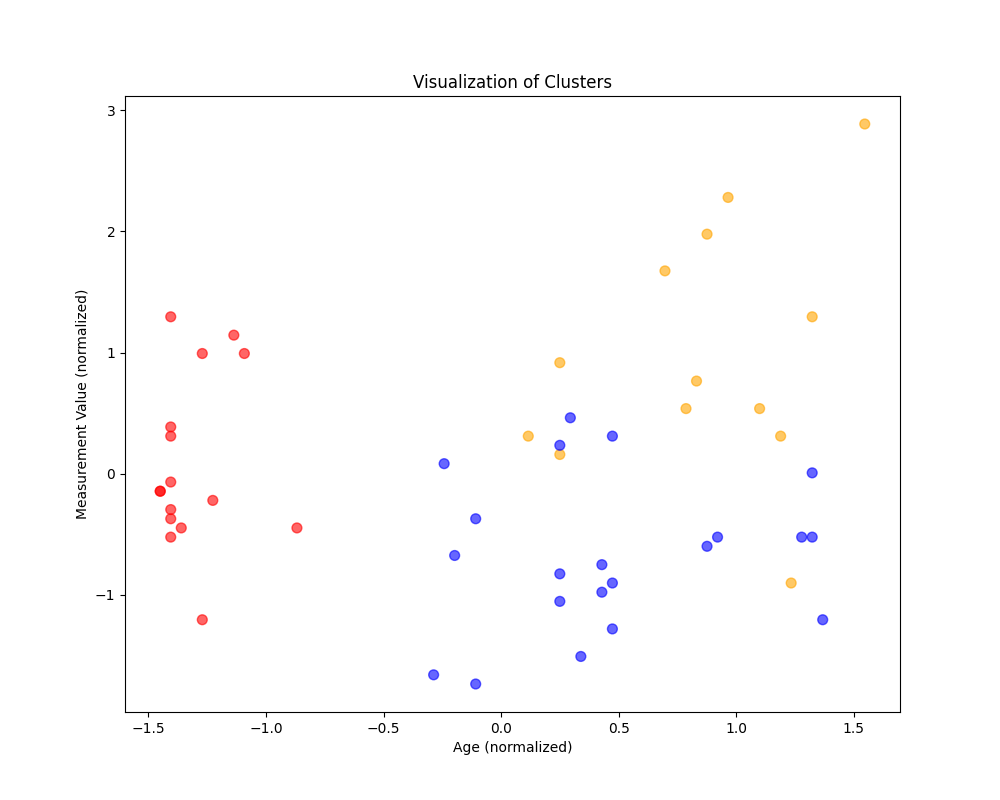
\includegraphics[width=0.9\textwidth]{Master Thesis/Plots/cluster_visualization_no_yellow.png}
\caption{Clustering visualization with features age and heart rate}
\label{figure:clusterageHR}
\end{figure}

\begin{figure}[h!]
\centering
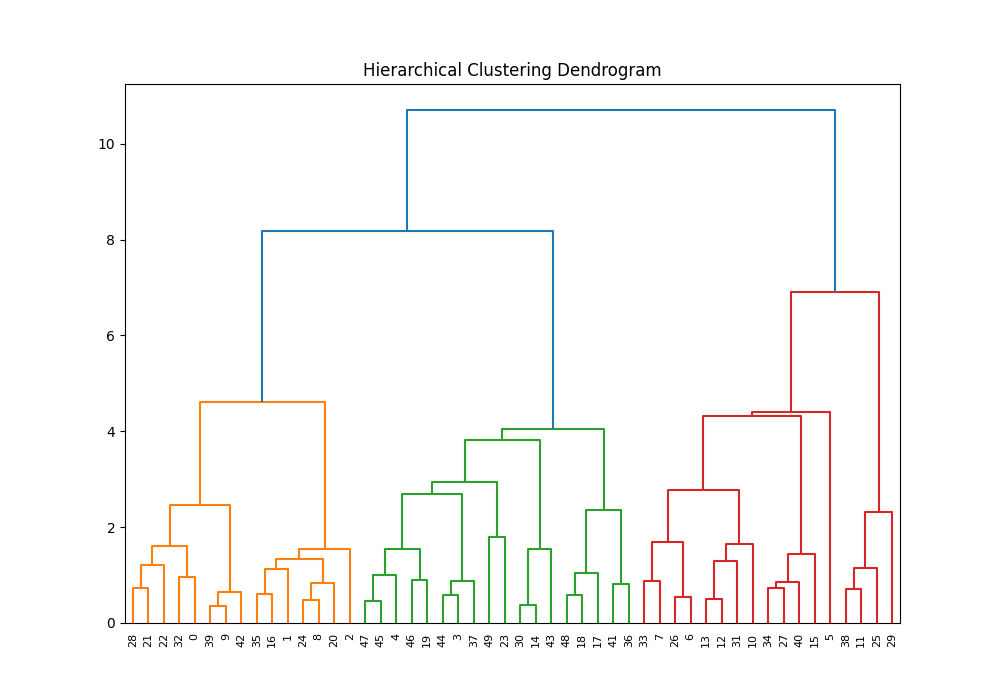
\includegraphics[width=0.9\textwidth]{Master Thesis/Plots/HierarchicalClustering_age+heartRate.png}
\caption{Hierarchical clustering visualization with features age and heart rate}
\label{figure:hirclusterageHR}
\end{figure}
\FloatBarrier

For hierarchical clustering, a silhouette score of 0.27 and a Davies-Bouldin score of 1.42 were obtained. The silhouette score, similar to the k-means result, indicates moderate clustering quality, with clusters that are not very compact or well-separated. The Davies-Bouldin score of 1.42 further indicates that the clusters are not optimally separated, suggesting average cluster separation and compactness.

The first figure ~\ref{figure:clusterageHR} shows the k-means clustering results, where the clusters are represented with different colors. The dispersion and overlap of points suggest that the clusters are not well-defined. The second figure ~\ref{figure:hirclusterageHR} illustrates the hierarchical clustering dendrogram, highlighting the relationships and distances between data points. The dendrogram shows that the clusters are not clearly separated, which is consistent with the silhouette and Davies-Bouldin scores.

Overall, the clustering results for both methods reveal that the features age and heart rate do not form well-defined clusters within the dataset. This could be attributed to the nature of the data, the choice of features, or the clustering method used. Further refinement in feature selection or alternative clustering approaches may be needed to achieve better-defined clusters but at this point we wanted to try other models as well.

\section{Analyzing the 6MWT Theory}

The aim of this section is to explore the correlation between age, distance, and heart rate using various classification and regression models. This analysis proofs or disproofs the hypothesis that age and heart rate can predict the distance traveled by subjects, which is central to the 6MWT theory.

\subsection{SVM Learning Model for 6MWT Features}

In this subsection, we investigate the potential of SVM learning to classify features associated with the 6MWT. The 6MWT is a widely used test to assess functional performance and predict cardiovascular and respiratory diseases by measuring the distance an individual can quickly walk on a flat, hard surface in six minutes. This test can also be used to determine the age of the subject based on the distance walked and the heart rate, and to intervene if the determined age differs too much from the calculated age. By analyzing our dataset, we aim to evaluate how well SVM models can predict health features based on the data collected during the 6MWT.

To explore the effectiveness of SVM learning for this purpose, various feature sets were tested. Using the first set of features, age and walked distance, the SVM model achieved an accuracy of 0.63. The detailed results are shown in the table below:

\FloatBarrier
\begin{table}[H]
\centering
\begin{tabular}{lrrrr}
\toprule
{} & precision & recall & f1-score & support \\
\midrule
no risk & 1.00 & 0.45 & 0.62 & 11.00 \\
risk & 0.45 & 1.00 & 0.62 & 5.00 \\
macro avg & 0.73 & 0.73 & 0.62 & 16.00 \\
weighted avg & 0.83 & 0.62 & 0.62 & 16.00 \\
\bottomrule
\end{tabular}
\caption{SVM model results with features age and distance}
\label{table:svmagedist}
\end{table}
\FloatBarrier

The SVM model's performance using age and distance as features yielded an overall accuracy of 0.62. For class 'no risk', the model achieved a perfect precision of 1.00, indicating it correctly identified all instances it classified as no risk. However, the recall for class 'no risk' was only 0.45, meaning the model missed more than half of the actual no-risk instances. Conversely, for class 'risk', the precision was 0.45, indicating a substantial number of false positives. The recall for class 'risk' was 1.00, showing that the model correctly identified all risk instances but at the cost of many false alarms. The macro average precision and recall were both 0.73, reflecting the model's mixed performance across the two classes, while the weighted averages highlight the same trend, emphasizing the imbalance in classification accuracy.

For the second set of features we used the age and the heart rate of the subjects. The SVM model also resulted in an accuracy of 0.63. The results are summarized in the following table:

\FloatBarrier
\begin{table}[H]
\centering
\begin{tabular}{lrrrr}
\toprule
{} & precision & recall & f1-score & support \\
\midrule
no risk & 1.00 & 0.45 & 0.62 & 11.00 \\
risk & 0.45 & 1.00 & 0.62 & 5.00 \\
macro avg & 0.73 & 0.73 & 0.62 & 16.00 \\
weighted avg & 0.83 & 0.62 & 0.62 & 16.00 \\
\bottomrule
\end{tabular}
\caption{SVM model results with features age and heart rate}
\label{table:svmageHR}
\end{table}
\FloatBarrier

Using age and heart rate as features, the SVM model achieved an accuracy of 0.62, mirroring the results obtained with age and distance. The precision for class 'no risk' remained perfect at 1.00, but the recall was low at 0.45, indicating the model effectively identified true negatives but missed many true positives. For class 'risk', the precision was 0.45, reflecting a significant number of false positives, while the recall was 1.00, indicating the model correctly identified all risk instances. The macro average precision and recall scores were both 0.73, similar to the previous feature set, highlighting the consistent but limited predictive power of the model. The weighted averages further illustrate the model's imbalance in performance across the two classes.

When we changed the features to distance and heart rate, the accuracy improved to 0.69, as shown in the following table:

\FloatBarrier
\begin{table}[H]
\centering
\begin{tabular}{lrrrr}
\toprule
{} & precision & recall & f1-score & support \\
\midrule
no risk & 0.69 & 1.00 & 0.81 & 11.00 \\
risk & 0.00 & 0.00 & 0.00 & 5.00 \\
macro avg & 0.34 & 0.50 & 0.41 & 16.00 \\
weighted avg & 0.47 & 0.69 & 0.56 & 16.00 \\
\bottomrule
\end{tabular}
\caption{SVM Results with Distance and Heart Rate}
\end{table}
\FloatBarrier

The combination of distance and heart rate improved the accuracy to 0.69. However, the recall for class 'risk' was zero, indicating that it failed to correctly identify any of the positive cases. This suggests that while the model can identify non-risk cases effectively, it struggles to detect risk cases using these features. The precision for class 'no risk' was 0.69 with a recall of 1.00, meaning the model identified all true negatives but failed to identify true positives for class 'risk'. The macro average indicates that the overall model performance is poor in detecting risk cases, emphasizing the need for better feature selection or model adjustment.

Finally, by incorporating all three features (distance, heart rate and age), the SVM model maintained an accuracy of 0.63, as shown in the table below:

\FloatBarrier
\begin{table}[H]
\centering
\begin{tabular}{lrrrr}
\toprule
{} & precision & recall & f1-score & support \\
\midrule
no risk & 1.00 & 0.45 & 0.62 & 11.00 \\
risk & 0.45 & 1.00 & 0.62 & 5.00 \\
macro avg & 0.73 & 0.73 & 0.62 & 16.00 \\
weighted avg & 0.83 & 0.62 & 0.62 & 16.00 \\
\bottomrule
\end{tabular}
\caption{SVM model results with features age, heart rate and distance}
\label{table:svmageHRdist}
\end{table}
\FloatBarrier

Including all three features (distance, heart rate and age) did not improve the accuracy, maintaining it at 0.62. The precision and recall values remained consistent with previous tests, indicating that the additional feature did not contribute significantly to the model's predictive capability. This suggests that while the model is effective in identifying non-risk cases, it struggles with detecting risk cases even with the inclusion of an additional feature.

When the feature 'leg length (cm)' was added, the performance worsened, with accuracy dropping to 0.50 across all sets. This indicates that including irrelevant or weakly correlated features can degrade the model's performance, highlighting the importance of feature selection in predictive modeling.

\subsection{Random Forest Model for 6MWT Features}

To classify the risk of subjects based on measured heart rate, distance, and age, the same model was used as in the previous subsection on RF with a few improvements. The features used in the initial model included heart rate and distance (measured by the Apple Watch Ultra), along with age (not measured by the Apple Watch Ultra). The model aimed to predict the risk classification of subjects without considering BMI.

The initial set of features resulted in an accuracy of 63\%. Detailed results are shown in the table below:

\begin{table}[H]
\centering
\begin{tabular}{lrrrr}
\toprule
{} & precision & recall & f1-score & support \\
\midrule
no risk & 0.58 & \textbf{0.88} & 0.70 & 8.00 \\
risk & \textbf{0.75} & 0.38 & 0.50 & 8.00 \\
macro avg & 0.67 & 0.63 & 0.60 & 16.00 \\
weighted avg & 0.67 & 0.63 & 0.60 & 16.00 \\
\bottomrule
\end{tabular}
\caption{RF classification with features distance, heart rate and age}
\label{table:RFdistHeartrateage}
\end{table}

The initial results in table ~\ref{table:RFdistHeartrateage} show moderate performance. The precision for the positive class 'risk' is 0.75, indicating that 75\% of the predicted positives are true positives. For the negative class 'no risk', the precision is 0.58. The recall for the negative class is high at 0.88, meaning the model correctly identifies 88\% of the true negatives. However, the recall for the positive class is low at 0.38, indicating that the model misses many true positives. The overall accuracy is 63\%, showing some predictive capability but room for improvement.

To further explore the impact of different features on model performance, several variations were tested. Initially, only heart rate and age were used, resulting in an accuracy of 50\%, indicating randomness and insufficient predictive power.

After that, we wanted to see if reducing the number of features might improve the results, so we used only age and distance. This approach led to an improved accuracy of 81\%, as shown in the table below:

\begin{table}[H]
\centering
\begin{tabular}{lrrrr}
\toprule
{} & precision & recall & f1-score & support \\
\midrule
no risk & 0.73 & \textbf{1.00} & 0.84 & 8.00 \\
risk & \textbf{1.00} & 0.63 & 0.77 & 8.00 \\
Macro Avg & 0.86 & 0.81 & 0.81 & 16.00 \\
Weighted Avg & 0.86 & 0.81 & 0.81 & 16.00 \\
\bottomrule
\end{tabular}
\caption{RF classification with features distance and age}
\label{table:RFdistage}
\end{table}

The results in table ~\ref{table:RFdistage} indicate a significant improvement, with an accuracy of 81\%. The precision for the positive class increased to 1.00, and the recall for the negative class remained perfect at 1.00, suggesting that age and distance are strong predictors for risk classification.

Interestingly, omitting heart rate data and using only age and distance improved the model's performance, suggesting that the heart rate data from the Apple Watch Ultra might not contribute significantly to risk prediction in this context. This implies that the model can achieve better results without relying on Apple Watch Ultra data, emphasizing the robustness of age and distance as key predictive features.

Testing with heart rate and distance again yielded an accuracy of 50\%, confirming the randomness of this feature set. This further highlights the potential inadequacy of heart rate data from the Apple Watch Ultra for effective risk prediction in this specific application.

\subsubsection{Optimizing the Random Forest Model}

To improve the accuracy of the RF model, we used Grid Search Cross-Validation (CV) to find the best hyperparameters. This process involved trying different combinations of features to find the most effective settings. The table below shows the optimization results, where negative scores represent the negative MSE. A lower score means better model performance.

\FloatBarrier
\begin{table}[h!]
\centering
\label{tab:optimization_results}
\begin{tabular}{>{\raggedright\arraybackslash}p{3.5cm} >{\raggedright\arraybackslash}p{6cm} r}
\toprule
\textbf{feature set} & \textbf{best parameters} & \textbf{best score} \\
\midrule
heart rate and distance & \texttt{max\_depth: None, max\_features: 'sqrt', min\_samples\_leaf: 1, min\_samples\_split: 10, n\_estimators: 200} & -0.4167 \\
\addlinespace
\textbf{age and distance} & \texttt{max\_depth: None, max\_features: 'sqrt', min\_samples\_leaf: 1, min\_samples\_split: 2, n\_estimators: 100} & \textbf{-0.2667} \\
\addlinespace
heart rate and age & \texttt{max\_depth: None, max\_features: 'sqrt', min\_samples\_leaf: 4, min\_samples\_split: 2, n\_estimators: 200} & -0.2833 \\
\addlinespace
\textbf{heart rate, distance, and age} & \texttt{max\_depth: None, max\_features: 'sqrt', min\_samples\_leaf: 1, min\_samples\_split: 2, n\_estimators: 100} & \textbf{-0.2667} \\
\bottomrule
\end{tabular}
\caption{RF optimization results with CV and different feature sets}
\label{table:RFoptiCV}
\end{table}
\FloatBarrier

The RF model includes several key hyperparameters that control its behavior and performance. The 'max\_depth' parameter limits the maximum depth of the trees, preventing overfitting by restricting the model's complexity. The 'max\_features' parameter dictates the number of features to consider when looking for the best split, which introduces randomness and reduces the risk of overfitting. The 'min\_samples\_leaf' parameter sets the minimum number of samples required to be at a leaf node, ensuring that each leaf has enough data to avoid learning from noise. The 'min\_samples\_split' parameter specifies the minimum number of samples needed to split an internal node, preventing splits that create overly specific branches. Lastly, the 'n\_estimators' parameter determines the number of trees in the forest, balancing model accuracy and computational efficiency by controlling the number of decision trees built in the RF. Properly tuning these hyperparameters is essential for developing a robust and well-generalizing RF model.

The table lists the best parameters and the corresponding scores for various feature combinations, highlighting the performance of each set measured and compared trough their MSE.

The feature set combining age and distance achieved the best performance, with a score of -0.2667. This indicates that these features are highly effective for the model, as reflected in the lowest negative mean squared error. The feature set incorporating heart rate, distance, and age also achieved the same best score of -0.2667, reinforcing the importance of age and distance in the model's predictions.

In contrast, the feature set of heart rate and distance yielded the worst performance with a score of -0.4167, suggesting that these features alone are less effective for accurate classification. The set of heart rate and age performed better than heart rate and distance but was still not as effective as age and distance alone, with a score of -0.2833.

In conclusion, the RF model's optimization results demonstrate that using age and distance as features provides the best classification accuracy. The hyperparameter tuning further enhanced the model's performance, indicating the significance of these features in predicting the risk of subjects. Future analysis will explore the impact of excluding data from certain devices, such as the Apple Watch Ultra, to understand potential limitations and improve the model's predictions.

\subsection{Regression Model for 6MWT Features}

We aimed to see if regression could yield better results than our previous models. Initially, we used age and heart rate as predictors to estimate the distance traveled by subjects. The resulting RMSE was 7.26, indicating that the predictions deviated from the actual values by approximately seven meters, which is relatively accurate.

\FloatBarrier
\begin{figure}[h!]
    \centering
    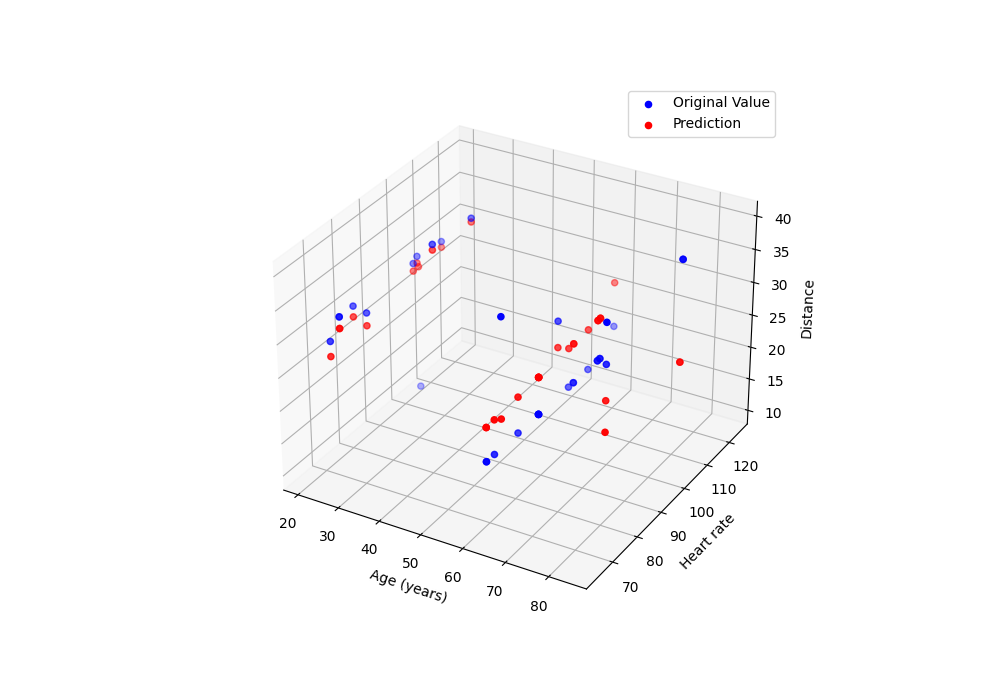
\includegraphics[width=0.9\textwidth]{Master Thesis/Plots/Distance_prediction.png}
    \caption{Distance prediction with regression based on features heart rate and age}
\label{figure:distregwithHRage}
\end{figure}
\FloatBarrier

Figure ~\ref{figure:distregwithHRage} shows a 3D scatter plot with age (years) on the X-axis, heart rate on the Z-axis, and distance on the Y-axis. The scatter plot visually demonstrates the alignment between the original and predicted values, indicating a moderate level of accuracy in the regression model. The dots are close to each other, what corresponds to our lower RMSE value.

To further improve the accuracy of the model, we applied gradient boosting regression. This approach resulted in a lower RMSE value of 4.65. Furthermore, this shows that the accuracy of the model varies by about 1.26 meters in different parts of the dataset. This variation suggests that the model performs more consistently in some scenarios or for certain patient groups.
We obtained this diagram: 

\FloatBarrier
\begin{figure}[h!]
    \centering
    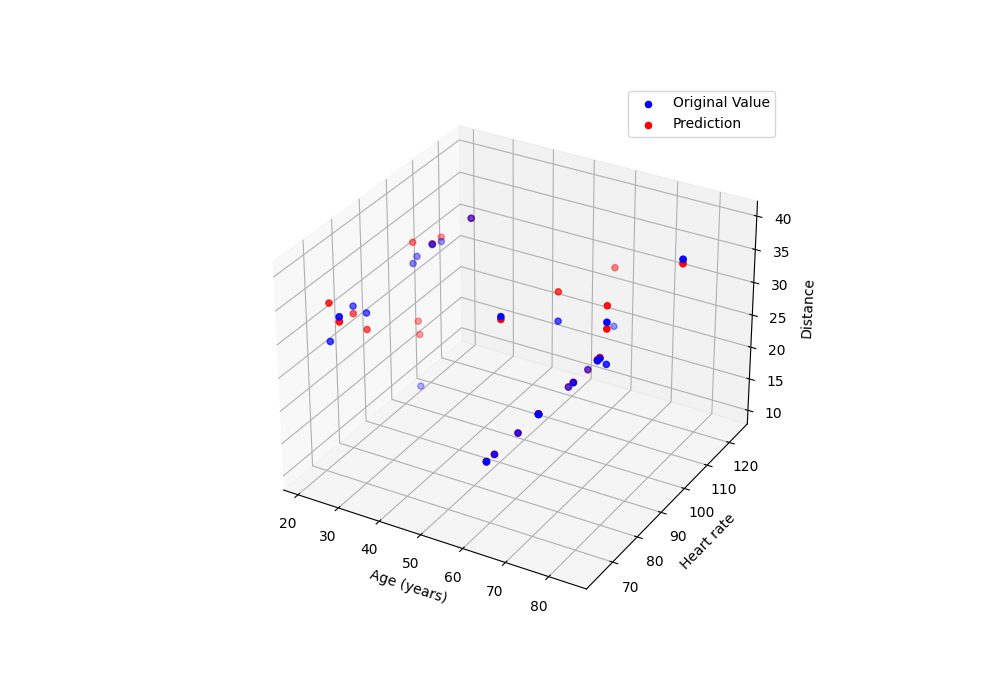
\includegraphics[width=0.9\textwidth]{Master Thesis/Plots/Proof_6MWT_prediction.png}
    \caption{Distance prediction with gradient boosting regression based on features heart rate and age}
    \label{figure:distGBregwithHRage}
\end{figure}
\FloatBarrier

Figure ~\ref{figure:distGBregwithHRage} shows a 3D scatter plot with again age (years) on the X-axis, heart rate on the Z-axis, and distance on the Y-axis. The scatter plot visually demonstrates the alignment between the original and predicted values, indicating a even better level of accuracy in the regression model. The dots are even closer to each other, what corresponds to our smaller RMSE value.

The GBR model outperforms the simple linear regression, as indicated by the tighter clustering of predicted points around the actual values and a lower RMSE value. These results suggest that using more sophisticated regression techniques can lead to more accurate predictions, supporting the correlation between age, heart rate, and distance traveled in the context of the 6MWT theory.

\subsubsection*{Model Performance Evaluation}

In this part of the work, we aim to verify the hypothesis from the previous section that boosting regression model might perform better for our dataset. Therefore, we will evaluate the performance of various regression models (linear regression, gradient boosting, XGBoost, CatBoost, and ensemble models) for each feature: heart rate, age and distance. Our analysis will focus on determining which model yields the best results for each feature by comparing their RMSE values.

The RMSE will be our primary metric for assessing model accuracy. RMSE measures the differences between values predicted by a model and the actual observed values, providing a clear indication of the model's prediction accuracy.

\subsubsection*{Heart Rate Prediction} 

\FloatBarrier
\begin{table}[htbp]
\centering
\begin{tabular}{@{}lc@{}}
\toprule
model & RMSE \\ 
\midrule
linear regression & \textbf{17.30} \\
gradient boosting regression & 19.62 \\
XGBoost regression & 18.77 \\
CatBoost regression & 17.60 \\
ensemble regression & 18.45 \\ 
\bottomrule
\end{tabular}
\caption{RMSE results for predicting heart rate feature with different regression models}
\end{table}
\FloatBarrier

The results indicate that the linear regression model performs the best in predicting heart rate, with an RMSE of 17.30. CatBoost regression follows closely with an RMSE of 17.60. The gradient boosting and XGBoost models shows slightly higher RMSE values of 19.62 and 18.77, respectively, indicating less accuracy compared to linear regression. The ensemble regression model performs moderately with an RMSE of 18.45.

\subsubsection*{Age Prediction} 
\FloatBarrier
\begin{table}[htbp]
\centering
\begin{tabular}{@{}lc@{}}
\toprule
model & RMSE\\ \midrule
linear regression & 21.50 \\
gradient boosting regression & 13.31 \\
XGBoost regression & 12.98 \\
CatBoost regression & \textbf{12.37} \\
ensemble regression & 12.59 \\ \bottomrule
\end{tabular}
\caption{RMSE results for predicting age feature with different regression models}
\end{table}
\FloatBarrier

The CatBoost regression achieves the lowest RMSE of 12.37, making it the most accurate model for predicting age. The XGBoost regression model closely follows with an RMSE of 12.98. Gradient boosting regression also performs well with an RMSE of 13.31. The linear regression model shows a significantly higher RMSE of 21.50, indicating less accuracy. The ensemble regression model has a decent performance with an RMSE of 12.59.

\newpage
\subsubsection*{Distance Prediction}
\FloatBarrier
\begin{table}[htbp]
\centering
\begin{tabular}{@{}lc@{}}
\toprule
model & RMSE \\ \midrule
linear regression & 7.26 \\
gradient boosting regression & 4.65 \\
XGBoost regression & \textbf{3.27} \\
CatBoost regression & 4.24 \\
ensemble regression & 3.62 \\ \bottomrule
\end{tabular}
\caption{RMSE results for predicting distance feature with different regression models}
\end{table}
\FloatBarrier

For distance prediction, the XGBoost regression model outperforms all others with the lowest RMSE of 3.27. The ensemble regression model also demonstrates high accuracy with an RMSE of 3.62. CatBoost regression and gradient boosting regression follow with RMSE values of 4.24 and 4.65, respectively. Linear regression has the highest RMSE of 7.26, indicating it was the least accurate model for this task.

The results of the regression model evaluations highlight that boosting models, particularly XGBoost and CatBoost, often provide superior performance compared to linear regression. For heart rate prediction, linear regression performed the best, whereas for age and distance predictions, boosting models outperformed others. This reinforces the importance of selecting appropriate models for different features to achieve the best predictive accuracy.

In the next steps, we will further investigate whether excluding certain features, especially those measured by the Apple Watch Ultra, could lead to better predictions, as indicated by some of our earlier findings. An additional consideration is whether including more data measured by the Apple Watch Ultra would be helpful.

\newpage

\section{Summary Table of Chapter Results}
\FloatBarrier
\notsotiny
\begin{longtable}{llrrrrr}
    \caption{Summary of all results in chapter 7 for various models and feature sets} \\
    \toprule
    \textbf{prediction task} & \textbf{features / metrics} & \textbf{precision} & \textbf{recall} & \textbf{f1-score} & \textbf{support} & \textbf{accuracy} \\
    \midrule
    \endfirsthead
    \caption[]{Summary of all results in chapter 7 for various models and feature sets (continued)} \\
    \toprule
    \textbf{prediction task} & \textbf{features / metrics} & \textbf{precision} & \textbf{recall} & \textbf{f1-score} & \textbf{support} & \textbf{accuracy} \\
    \midrule
    \endhead
    \bottomrule
    \endfoot
    \multirow{6}{*}{risk indicator (RF)} 
    & age, weight, height, step count & & & & & 0.94 \\
    & no risk & 0.92 & 1.00 & 0.96 & 11.00 & \\
    & risk & 1.00 & 0.80 & 0.89 & 5.00 & \\
    & macro avg & 0.96 & 0.90 & 0.92 & 16.00 & \\
    & weighted avg & 0.94 & 0.94 & 0.94 & 16.00 & \\
    \midrule
    \multirow{6}{*}{risk indicator (RF)} 
    & age, heart rate (max, min, avg), step count & & & & & 0.75 \\
    & no risk & 0.89 & 0.73 & 0.80 & 11.00 & \\
    & risk & 0.57 & 0.80 & 0.67 & 5.00 & \\
    & macro avg & 0.73 & 0.76 & 0.73 & 16.00 & \\
    & weighted avg & 0.79 & 0.75 & 0.76 & 16.00 & \\
    \midrule
    \multirow{6}{*}{risk indicator (RF)} 
    & heart rate (min, max, avg), age, BMI > 25 & & & & & 0.50 \\
    & no risk & 0.50 & 0.75 & 0.60 & 8.00 & \\
    & risk & 0.50 & 0.25 & 0.33 & 8.00 & \\
    & macro avg & 0.50 & 0.50 & 0.47 & 16.00 & \\
    & weighted avg & 0.50 & 0.50 & 0.47 & 16.00 & \\
    \midrule
    \multirow{6}{*}{risk indicator (GBM)} 
    & heart rate (min, max, avg), age, BMI > 25 & & & & & 0.81 \\
    & no risk & 0.78 & 0.88 & 0.82 & 8.00 & \\
    & risk & 0.86 & 0.75 & 0.80 & 8.00 & \\
    & macro avg & 0.82 & 0.81 & 0.82 & 16.00 & \\
    & weighted avg & 0.82 & 0.81 & 0.82 & 16.00 & \\
    \midrule
    \multirow{6}{*}{subject/patient (RF)} 
    & age, distance & & & & & 0.94 \\
    & patient & 0.91 & 1.00 & 0.95 & 10.00 & \\
    & subject & 1.00 & 0.83 & 0.91 & 6.00 & \\
    & macro avg & 0.95 & 0.92 & 0.93 & 16.00 & \\
    & weighted avg & 0.94 & 0.94 & 0.94 & 16.00 & \\
    \midrule
    \multirow{6}{*}{subject/patient (RF)} 
    & age, heart rate & & & & & 0.94 \\
    & patient & 0.91 & 1.00 & 0.95 & 10.00 & \\
    & subject & 1.00 & 0.83 & 0.91 & 6.00 & \\
    & macro avg & 0.95 & 0.92 & 0.93 & 16.00 & \\
    & weighted avg & 0.94 & 0.94 & 0.94 & 16.00 & \\
    \midrule
    \multirow{6}{*}{subject/patient (RF)} 
    & distance, heart rate & & & & & 0.63 \\
    & patient & 0.62 & 1.00 & 0.77 & 10.00 & \\
    & subject & 0.00 & 0.00 & 0.00 & 6.00 & \\
    & macro avg & 0.31 & 0.50 & 0.38 & 16.00 & \\
    & weighted avg & 0.39 & 0.62 & 0.48 & 16.00 & \\
    \midrule
    \multirow{6}{*}{subject/patient (RF)} 
    & age, distance, heart rate & & & & & 0.94 \\
    & patient & 0.91 & 1.00 & 0.95 & 10.00 & \\
    & subject & 1.00 & 0.83 & 0.91 & 6.00 & \\
    & macro avg & 0.95 & 0.92 & 0.93 & 16.00 & \\
    & weighted avg & 0.94 & 0.94 & 0.94 & 16.00 & \\
    \midrule
    \multirow{4}{*}{heart rate prediction (LR)} 
    & height, weight & \multicolumn{4}{c}{RMSE: 21.92} & \\
    & leg length, distance & \multicolumn{4}{c}{RMSE: 20.76} & \\
    & min heart rate & \multicolumn{4}{c}{RMSE: 2.64} & \\
    & max heart rate, min heart rate, weight & \multicolumn{4}{c}{RMSE: 1.57} & \\
    & max heart rate, min heart rate, weight, age & \multicolumn{4}{c}{RMSE: 17.01} & \\
    \midrule
    \multirow{6}{*}{subject/patient (Logistic Regression)} 
    & weight, age & & & & & 0.94 \\
    & patient & 0.91 & 1.00 & 0.95 & 10.00 & \\
    & subject & 1.00 & 0.83 & 0.91 & 6.00 & \\
    & macro avg & 0.95 & 0.92 & 0.93 & 16.00 & \\
    & weighted avg & 0.94 & 0.94 & 0.94 & 16.00 & \\
    %\midrule
    \newpage
    \multirow{1}{*}{deep learning (heart rate prediction)} 
    & age, distance & \multicolumn{4}{c}{MSE: 1.10} & \\
    \midrule
    \multirow{1}{*}{deep learning (distance prediction)} 
    & age, heart rate & \multicolumn{4}{c}{MSE: 0.59} & \\
    \midrule
    \multirow{1}{*}{deep learning (age prediction)} 
    & heart rate, distance & \multicolumn{4}{c}{MSE: 0.60} & \\
    \midrule
    \multirow{6}{*}{SVM (risk prediction)} 
    & age, distance & & & & & 0.63 \\
    & no risk & 1.00 & 0.45 & 0.62 & 11.00 & \\
    & risk & 0.45 & 1.00 & 0.62 & 5.00 & \\
    & macro avg & 0.73 & 0.73 & 0.62 & 16.00 & \\
    & weighted avg & 0.83 & 0.62 & 0.62 & 16.00 & \\
    \midrule
    \multirow{6}{*}{SVM (risk prediction)} 
    & age, heart rate & & & & & 0.63 \\
    & no risk & 1.00 & 0.45 & 0.62 & 11.00 & \\
    & risk & 0.45 & 1.00 & 0.62 & 5.00 & \\
    & macro avg & 0.73 & 0.73 & 0.62 & 16.00 & \\
    & weighted avg & 0.83 & 0.62 & 0.62 & 16.00 & \\
    \midrule
    \multirow{6}{*}{SVM (risk prediction)} 
    & distance, heart rate & & & & & 0.69 \\
    & no risk & 0.69 & 1.00 & 0.81 & 11.00 & \\
    & risk & 0.00 & 0.00 & 0.00 & 5.00 & \\
    & macro avg & 0.34 & 0.50 & 0.41 & 16.00 & \\
    & weighted avg & 0.47 & 0.69 & 0.56 & 16.00 & \\
    \midrule
    \multirow{6}{*}{SVM (risk prediction)} 
    & age, distance, heart rate & & & & & 0.63 \\
    & no risk & 1.00 & 0.45 & 0.62 & 11.00 & \\
    & risk & 0.45 & 1.00 & 0.62 & 5.00 & \\
    & macro avg & 0.73 & 0.73 & 0.62 & 16.00 & \\
    & weighted avg & 0.83 & 0.62 & 0.62 & 16.00 & \\
    \midrule
    \multirow{4}{*}{optimization (RF)} 
    & heart rate, distance & \multicolumn{4}{c}{best score: -0.4167} & \\
    & age, distance & \multicolumn{4}{c}{best score: -0.2667} & \\
    & heart rate, age & \multicolumn{4}{c}{best score: -0.2833} & \\
    & heart rate, distance, age & \multicolumn{4}{c}{best score: -0.2667} & \\
    \midrule
    \multirow{3}{*}{regression (RMSE)} 
    & age, heart rate (distance prediction) & \multicolumn{4}{c}{RMSE: 7.26} & \\
    & age, heart rate (gradient boosting) & \multicolumn{4}{c}{RMSE: 4.65} & \\
    \midrule
    \multirow{6}{*}{regression (heart rate prediction)} 
    & heart rate, age and distance & \\
    & linear regression & \multicolumn{4}{c}{RMSE: 17.30} & \\
    & gradient boosting regression& \multicolumn{4}{c}{RMSE: 19.62} & \\
    & XGBoost regression & \multicolumn{4}{c}{RMSE: 18.77} & \\
    & CatBoost regression & \multicolumn{4}{c}{RMSE: 17.60} & \\
    & ensemble regression & \multicolumn{4}{c}{RMSE: 18.45} & \\
    \midrule
    \multirow{6}{*}{regression (age prediction)}
    & heart rate, age and distance &   \\
    & linear regression & \multicolumn{4}{c}{RMSE: 21.50} & \\
    & gradient boosting regression & \multicolumn{4}{c}{RMSE: 13.31} & \\
    & XGBoost regression & \multicolumn{4}{c}{RMSE: 12.98} & \\
    & CatBoost regression & \multicolumn{4}{c}{RMSE: 12.37} & \\
    & ensemble regression & \multicolumn{4}{c}{RMSE: 12.59} & \\
    \midrule
    \multirow{6}{*}{regression (distance prediction)} 
    & heart rate, age and distance &  \\
    & linear regression & \multicolumn{4}{c}{RMSE: 7.26} & \\
    & gradient boosting regression & \multicolumn{4}{c}{RMSE: 4.65} & \\
    & XGBoost regression & \multicolumn{4}{c}{RMSE: 3.27} & \\
    & CatBoost regression & \multicolumn{4}{c}{RMSE: 4.24} & \\
    & ensemble regression & \multicolumn{4}{c}{RMSE: 3.62} & \\
    \bottomrule
\end{longtable}
\FloatBarrier
\normalsize
\chapter{Improving Model Performance with additional Health Data}
\label{cha:resultsaddFeatures}

To improve the accuracy and robustness of our health data analysis, this chapter focuses on integrating additional health metrics into the dataset. In chapter ~\ref{cha:results}, we primarily worked with data measured by the Apple Watch Ultra, excluding some crucial information from the study protocols. Now, we aim to enhance our analysis by incorporating all available data, including those from study protocols and additional Apple Watch Ultra measurements. This comprehensive approach will allow us to evaluate how these extra features impact the performance of our predictive models and provide a deeper understanding of health trends and risk factors.

\section{Additional Data Features}

In this part of the work, we focus on integrating the 6MWT documentation for each subject. During this process, we discovered significant discrepancies in the distance measurements recorded by the Apple Watch Ultra. 

\subsection{Additional Distance Data}

Initially, we calculated the real distance by multiplying the leg length by the number of steps taken, where the 'Steps' column represents the difference between the 'Steps (before)' and 'Steps (after)' columns. This resulted in three different distance metrics: 'Calculated m', 'Distance (km)' and 'real\_Distance'.
The term 'leg length' encompasses the distance from the heel to the inner pubic bone (as detailed in the study protocol). All columns related to steps were published in the shared table. The 'Calculated m' values were also entered into the shared table and the values 'Distance (km)' was measured using the Apple Watch Ultra, and the 'real distance' was computed manually, as explained in the text. 
These metrics were then plotted for visual comparison to evaluate the discrepancies.

\FloatBarrier
\begin{figure}[h!]
    \centering
    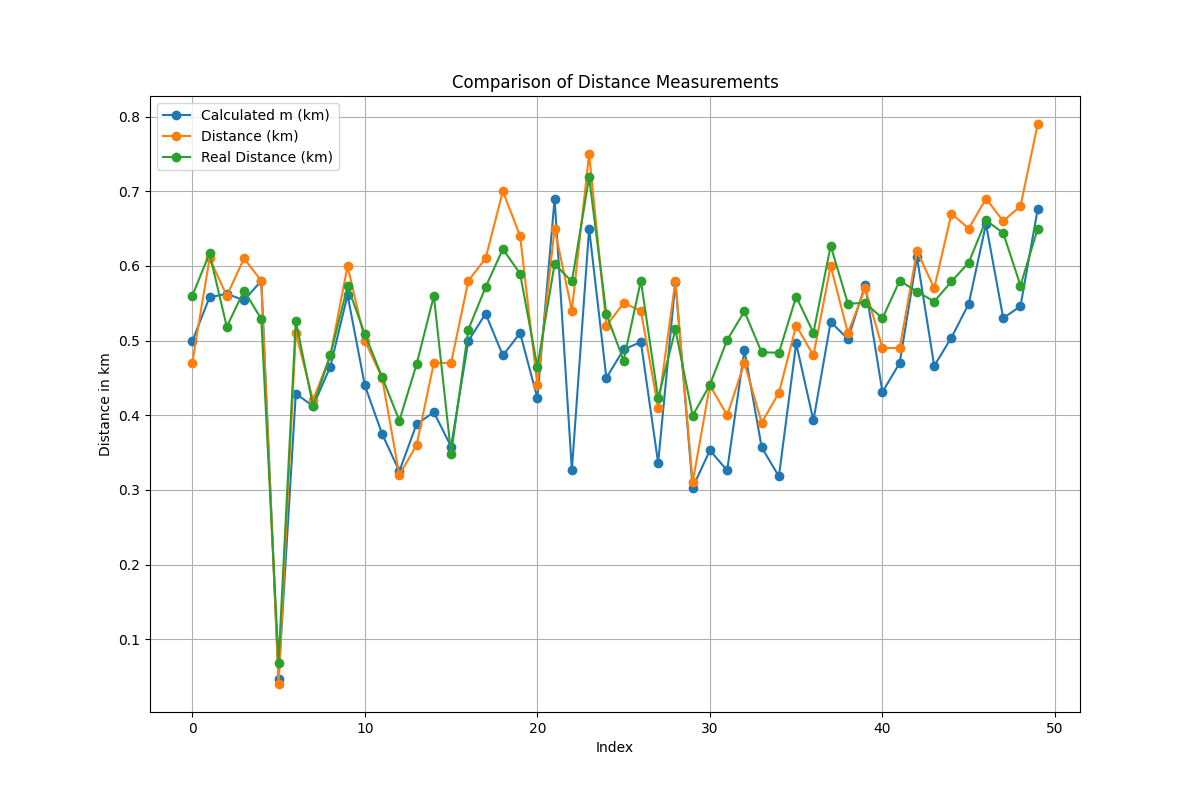
\includegraphics[width=0.9\textwidth]{Master Thesis/Plots/distance_comparison_plot.png}
    \caption{Comparison of measured distances 'Distance (km)', ’real_Distance’ and ’Calculated m’}
    \label{fig:distance_comparison_plot}
\end{figure}
\FloatBarrier

The differences between these measurements are calculated as percentages:
\begin{itemize}
    \item The highest difference between 'Calculated m' and 'Distance (km)' was 17.5\%.
    \item The highest difference between 'Calculated m' and 'real\_Distance' was 14.51\%.
    \item The highest difference between 'Distance (km)' and 'real\_Distance' was 34.94\%.
\end{itemize}

We have identified significant discrepancies between the actual distance traveled and the distance measured by the Apple Watch Ultra. Due to these large variations, we decided to use only the calculated distance for further analysis. This calculated distance is derived from the number of steps recorded by the Apple Watch Ultra and the leg length, thus partially utilizing Apple Watch Ultra data. Additionally, in this chapter, our focus is on using data measured by the Apple Watch Ultra to demonstrate that we can achieve better results.

\subsection{Additional Heart Rate and Blood Pressure Data}

To incorporate additional health metrics into our analysis, we decided to include blood pressure readings, as these provide valuable insights into a person's health. We manually added these values to the dataset from paper records and categorized them according to standard medical guidelines found online. These categories were then converted into numerical classes to facilitate their use in our models.

We categorized the blood pressure based on systolic (upper number) and diastolic (lower number) readings, measured in millimeters of mercury (mm Hg) ~\cite{heartUnderstandingBlood}:
\begin{itemize}
    \item \textbf{Normal blood pressure}: Systolic $<$ 120 mm Hg and diastolic $<$ 80 mm Hg, indicating a healthy heart condition and lower risk of cardiovascular diseases.
    \item \textbf{Elevated blood pressure}: Systolic 120-129 mm Hg and diastolic $<$ 80 mm Hg, indicating a higher than normal range but not yet hypertensive.
    \item \textbf{Hypertension Stage 1}: Systolic 130-139 mm Hg or diastolic 80-89 mm Hg, requiring lifestyle modifications and possibly medication.
    \item \textbf{Hypertension Stage 2}: Systolic $\geq$ 140 mm Hg or diastolic $\geq$ 90 mm Hg, necessitating more intensive treatment.
    \item \textbf{Hypertensive crisis}: Systolic $>$ 180 mm Hg and/or diastolic $>$ 120 mm Hg, a critical condition needing immediate medical intervention to prevent life-threatening complications such as organ damage or stroke.
\end{itemize}

We then added an additional column, alongside the columns for blood pressure before and after the 6MWT, to classify each subject's blood pressure. This classification helped us better understand the distribution of blood pressure among our subjects. The distribution of these categorized blood pressure values is illustrated in the following plot:

\FloatBarrier
\begin{figure}[h!]
    \centering
    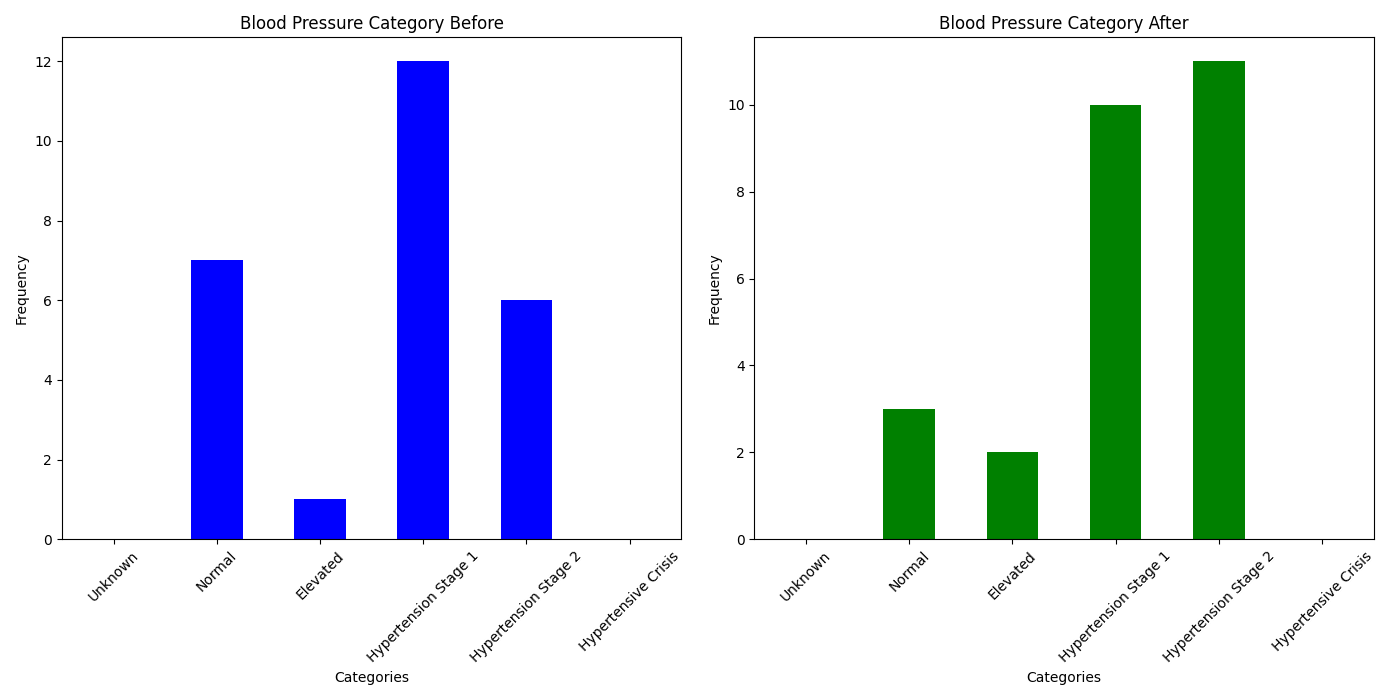
\includegraphics[width=1.0\textwidth]{Master Thesis/Plots/BloodPressure.png}
    \caption{Distribution of blood pressure categories}
    \label{fig:blood_pressure_distribution}
\end{figure}
\FloatBarrier

From the distribution, it is evident that there are no subjects in the 'Hypertensive Crisis' category, which is positive. However, a notable number of subjects fall into 'Hypertension Stage 1' and 'Hypertension Stage 2' categories, indicating a prevalence of elevated blood pressure and potential health risks within the study population. 

\subsection{Sex-Specific Data Analysis}

Additional information regarding the sex of the subjects was incorporated into the dataset from the documentation. We extracted details from the study, including sex and added them to the CSV file. One of our primary objectives was to investigate whether the heart rate of female subjects is generally higher than that of male subjects. To achieve an accurate analysis, we included 40 heart rate measurements for each subject in the dataset, with each value represented in a separate column. The information of the sex was manually entered as it was initially provided on paper.

The following plots visualize the measured heart rate for each male and female subject:

\FloatBarrier
\begin{figure}[h!]
  \centering
  \begin{minipage}[b]{0.9\linewidth}
    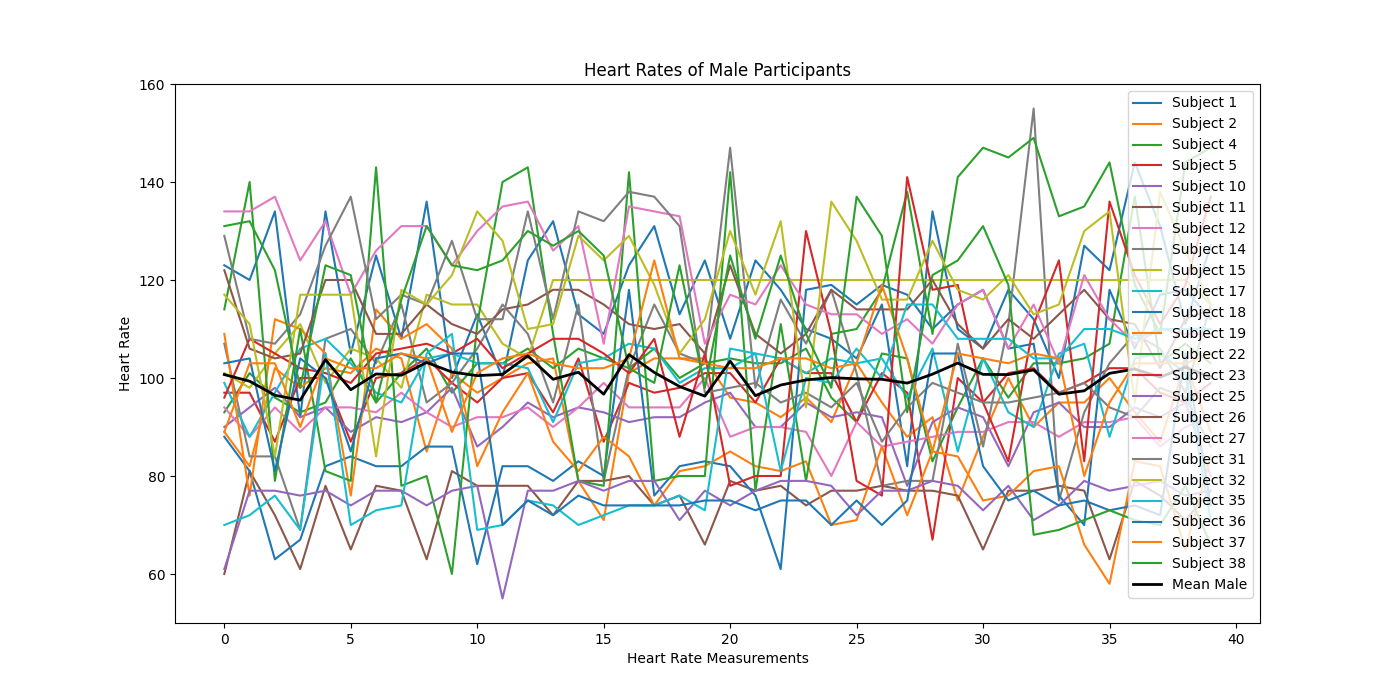
\includegraphics[width=\linewidth]{Master Thesis/Plots/comparison_plot_male.png}
    \caption{Visualization of the measured heart rate of each male subject and the measured mean in black}
    \label{fig:allmeashrdatamale}
  \end{minipage}
  \quad % Space between the images
  \begin{minipage}[b]{0.9\linewidth}
    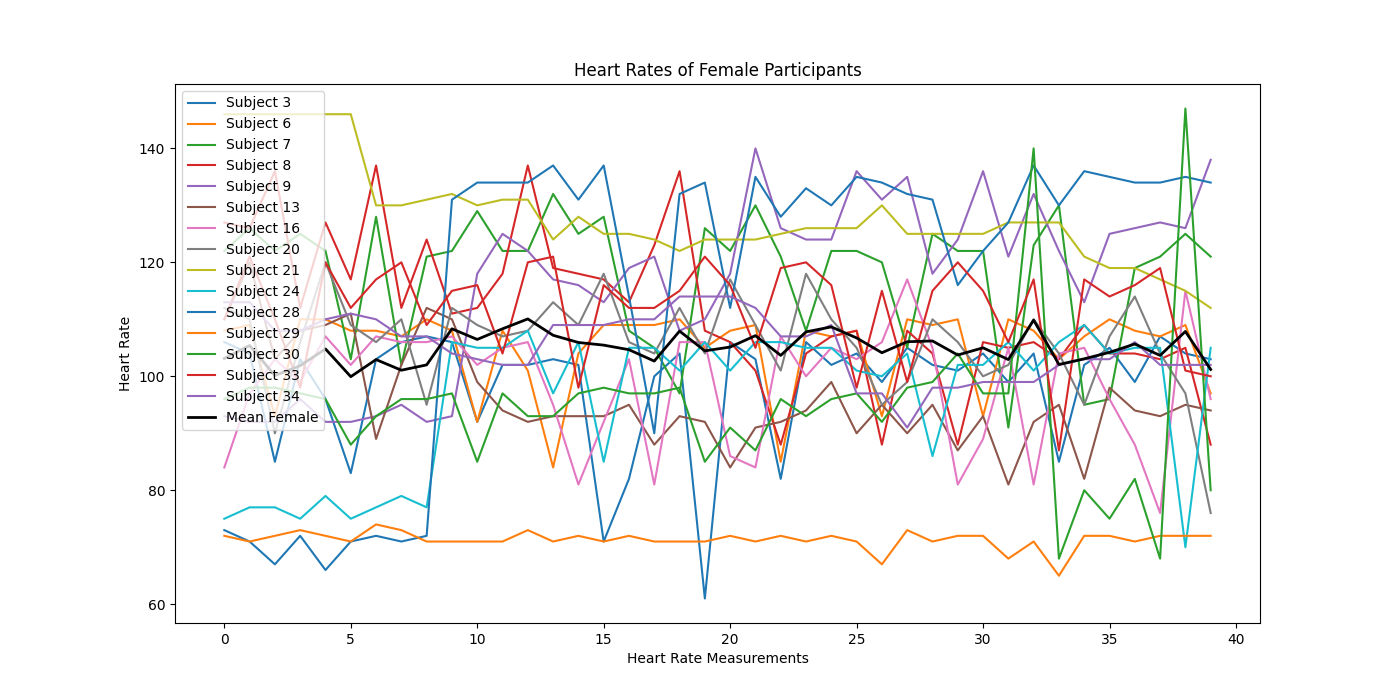
\includegraphics[width=\linewidth]{Master Thesis/Plots/comparison_plot_female.png}
    \caption{Visualization of the measured heart rate of each female subject and the measured mean in black}
    \label{fig:allmeashrdatafemale}
  \end{minipage}
\end{figure}
\FloatBarrier

Figure ~\ref{fig:allmeashrdatamale} and ~\ref{fig:allmeashrdatafemale} indicate that the heart rate patterns for both male and female subjects vary significantly. In each plot, individual lines represent the heart rate measurements for each subject across 40 instances. The black line represents the mean heart rate for all male and female subjects, providing a clear comparison of average heart rates between sex.

Figure ~\ref{fig:allmeashrdatafemale} presents the heart rates of female participants.
Each colored line represents the heart rate measurements of an individual female subject.
Similar to the male subjects in figure ~\ref{fig:allmeashrdatamale}, the black line represents the mean heart rate across all female subjects, indicating the overall trend and average heart rate pattern for females.

\FloatBarrier
\begin{figure}[h!]
  \centering
    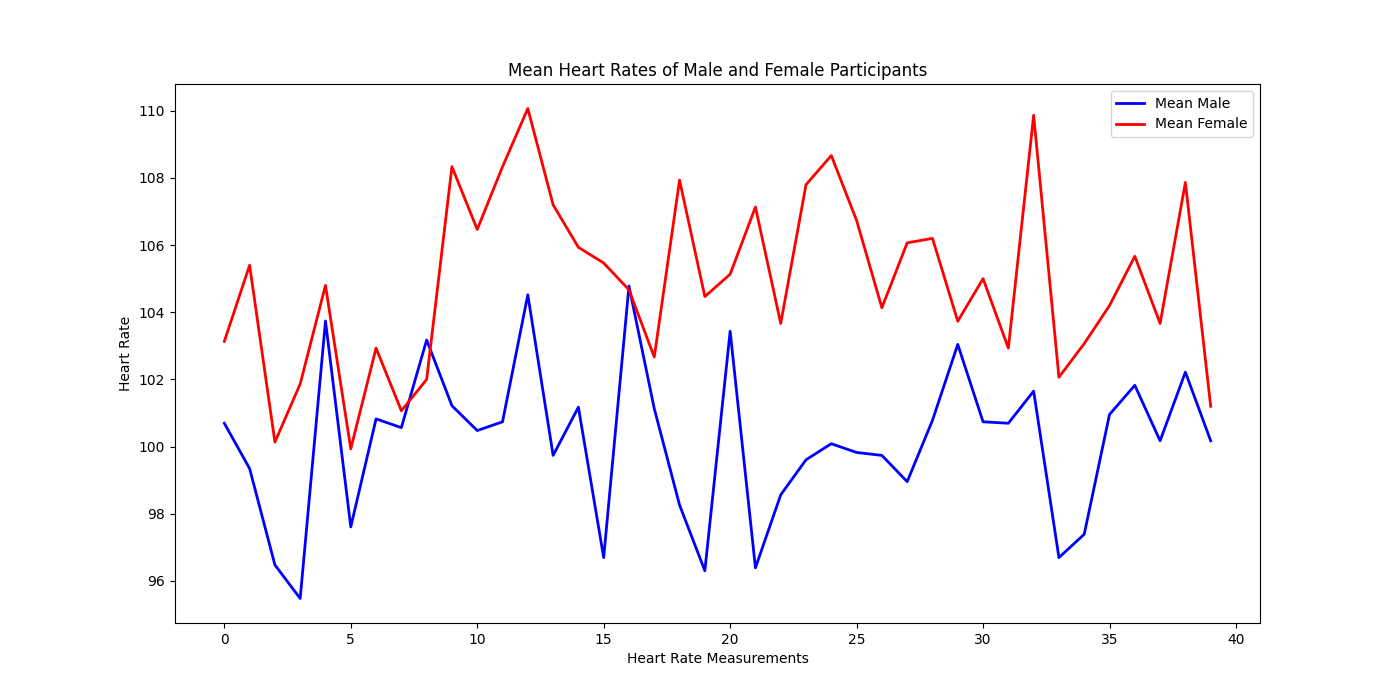
\includegraphics[width=1.0\linewidth]{Master Thesis/Plots/comparison_plot_mean_maleVSfemale.png}
    \caption{Mean heart rate comparison between male and female subjects}
    \label{fig:avhHRmalefemale}
\end{figure}
\FloatBarrier

Figure ~\ref{fig:avhHRmalefemale} highlights potential differences in cardiovascular responses between sex. It is evident that female subjects generally have higher mean heart rates compared to male subjects throughout the measurement period. This trend could indicate variations in cardiovascular health or fitness levels between the two groups. The fluctuations in the lines suggest variability in heart rates, with some overlap in certain intervals but a clear distinction in others. This visualization helps in understanding the general heart rate patterns and differences between male and female subjects.

\section{Supervised Learning Models}

We now evaluate the performance of supervised learning models on our dataset, including the information from the documentation and 10 heart rate measurements per subject. Our goal is to determine how well these models can predict health metrics based on this enriched data.

\subsection{Random Forest}
First we aimed to predict the sex of subjects using a combination of features including age, height, weight (not measured by the Apple Watch Ultra), and heart rates. We focused on the heart rates during the 6MWT, before, and after the test and even the blood pressure before and after the test. Utilizing the RF classifier model, we achieved an accuracy of 1.0. The detailed results are as follows:

\begin{table}[H]
\centering
\begin{tabular}{lrrrr}
\toprule
{} &  precision &  recall &  f1-score &  support \\
\midrule
female       &        1.0 &     1.0 &       1.0 &      2.0 \\
male         &        1.0 &     1.0 &       1.0 &      4.0 \\
macro avg    &        1.0 &     1.0 &       1.0 &      6.0 \\
weighted avg &        1.0 &     1.0 &       1.0 &      6.0 \\
\bottomrule
\end{tabular}
\caption{RF sex classification with all given features and 10 heart rate values}
\label{table:RFageHeartrate10weightheigt}
\end{table}

The results in table ~\ref{table:RFageHeartrate10weightheigt} from the RF model for predicting sex achieves perfect scores across all metrics. The precision of the model is 1.0 for both female and male subjects, indicating that every prediction made by the model for both sex was correct. The recall is also 1.0 for both female and male subjects, meaning that the model successfully identified all actual instances of both sex. The f1-score, which is the harmonic mean of precision and recall, is 1.0 for both sex, reflecting the model's perfect balance between precision and recall.

The support indicates the number of actual instances for each class in the test set, with two instances of female and four instances of male subjects. The overall accuracy of the model is 1.0, meaning the model correctly predicted the sex for all subjects in the test set. Both macro average and weighted average for precision, recall, and f1-score are also perfect at 1.0, demonstrating that the model performs consistently well across both classes.

These outstanding results suggest that the chosen features (age, height, weight, and heart rates) are highly effective in predicting sex. To further understand these results, we analyzed the importance of each feature in the model's decision-making process. The following plot illustrates the feature importance in the sex predictions:

\FloatBarrier
\begin{figure}[h!]
    \centering
    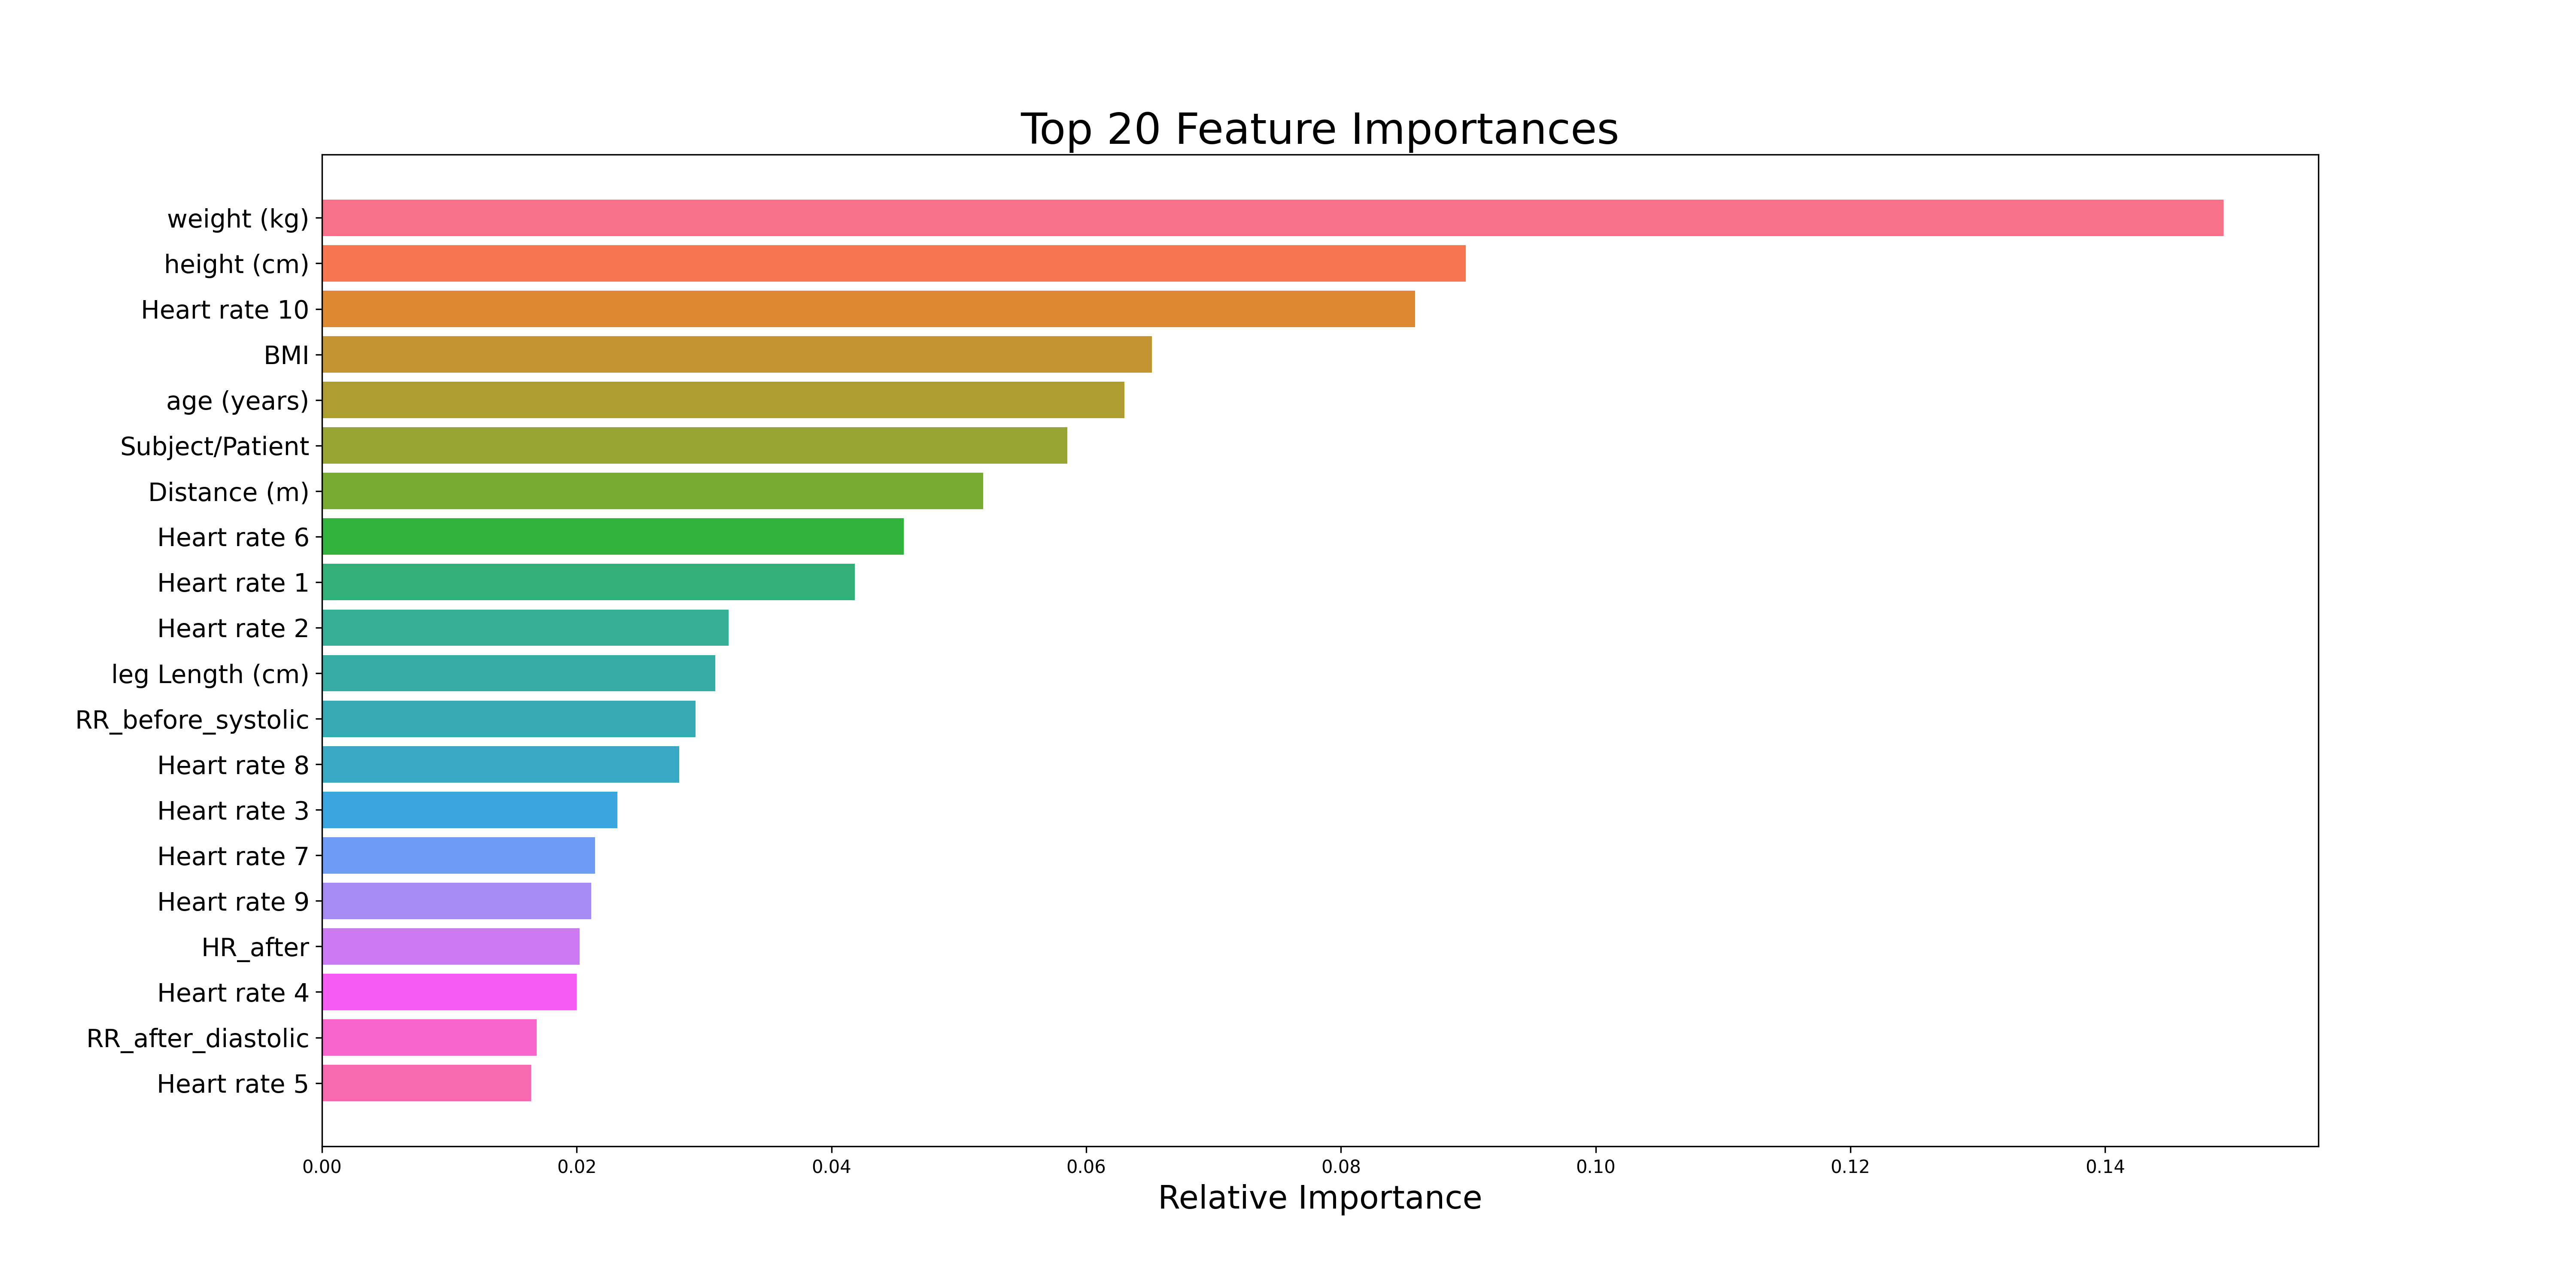
\includegraphics[width=1.0\textwidth]{Master Thesis/Plots/random_forest_top20_feature_importances_gender_oldData.png}
    \caption{Feature importance for sex prediction using RF with all given features and 10 heart rate values}
    \label{fig:featureimportanceRFsex10}
\end{figure}
\FloatBarrier

Figure ~\ref{fig:featureimportanceRFsex10} reveals that height and weight are the most important features for accurate sex prediction. Additionally, heart rates, particularly the latest measurements, age, and blood pressure before and after the 6MWT, are essential for achieving a perfect score with the RF model. As well we added features like active and basal energy burned. We have added these functions by summing up all the values of the energy type, whether basal or active. These are all values measured by the Apple Watch Ultra.

The supposedly excellent results are still questionable. Because of the six most important features for the prediction, only one feature is measured by the Apple Watch Ultra. However, we want to show that the Apple Watch Ultra delivers good and, above all, important data for the ML area, so we need to make further optimizations here. We expanded the dataset with additional heart rate data (100 measured heart rate values per subject) and another feature, to predict the sex of the subjects. This model achieved an accuracy of 78\%. The detailed results are shown below:

\begin{table}[H]
\centering
\begin{tabular}{lrrrr}
\toprule
{} &  precision &    recall &  f1-score &   support \\
\midrule
male            &   0.71 &  1.00 &  0.83 &  5.0 \\
female            &   1.00 &  0.50 &  0.67 &  4.0 \\
macro avg    &   0.86 &  0.75 &  0.75 &  9.0 \\
weighted avg &   0.84 &  0.78 &  0.76 &  9.0 \\
\bottomrule
\end{tabular}
\caption{RF sex classification with all given features and 100 heart rate values}
\label{table:RFageHeartrate100weightheigt}
\end{table}

The results from the RF classifier in table ~\ref{table:RFageHeartrate100weightheigt} with additional features are promising. The precision for class 'male' is 0.71, with a recall of 1.00, indicating that the model correctly identified all instances of this class. The f1-score for class 'male' is 0.83. For class 'female', the precision is 1.00, with a recall of 0.50, and an f1-score of 0.67.

Overall, the model achieved an accuracy of 0.78, meaning it correctly predicted the risk classification for 78\% of the subjects in the test set. The macro averages for precision, recall, and f1-score are 0.86, 0.75, and 0.75, respectively. The weighted averages are 0.84 for precision, 0.78 for recall, and 0.76 for f1-score.

These results suggest that the additional features have enhanced the model's predictive capability. To understand the impact of each feature, we analyzed their importance in the model's decision-making process. The following graph illustrates the feature importance:
\FloatBarrier
\begin{figure}[h!]
    \centering
    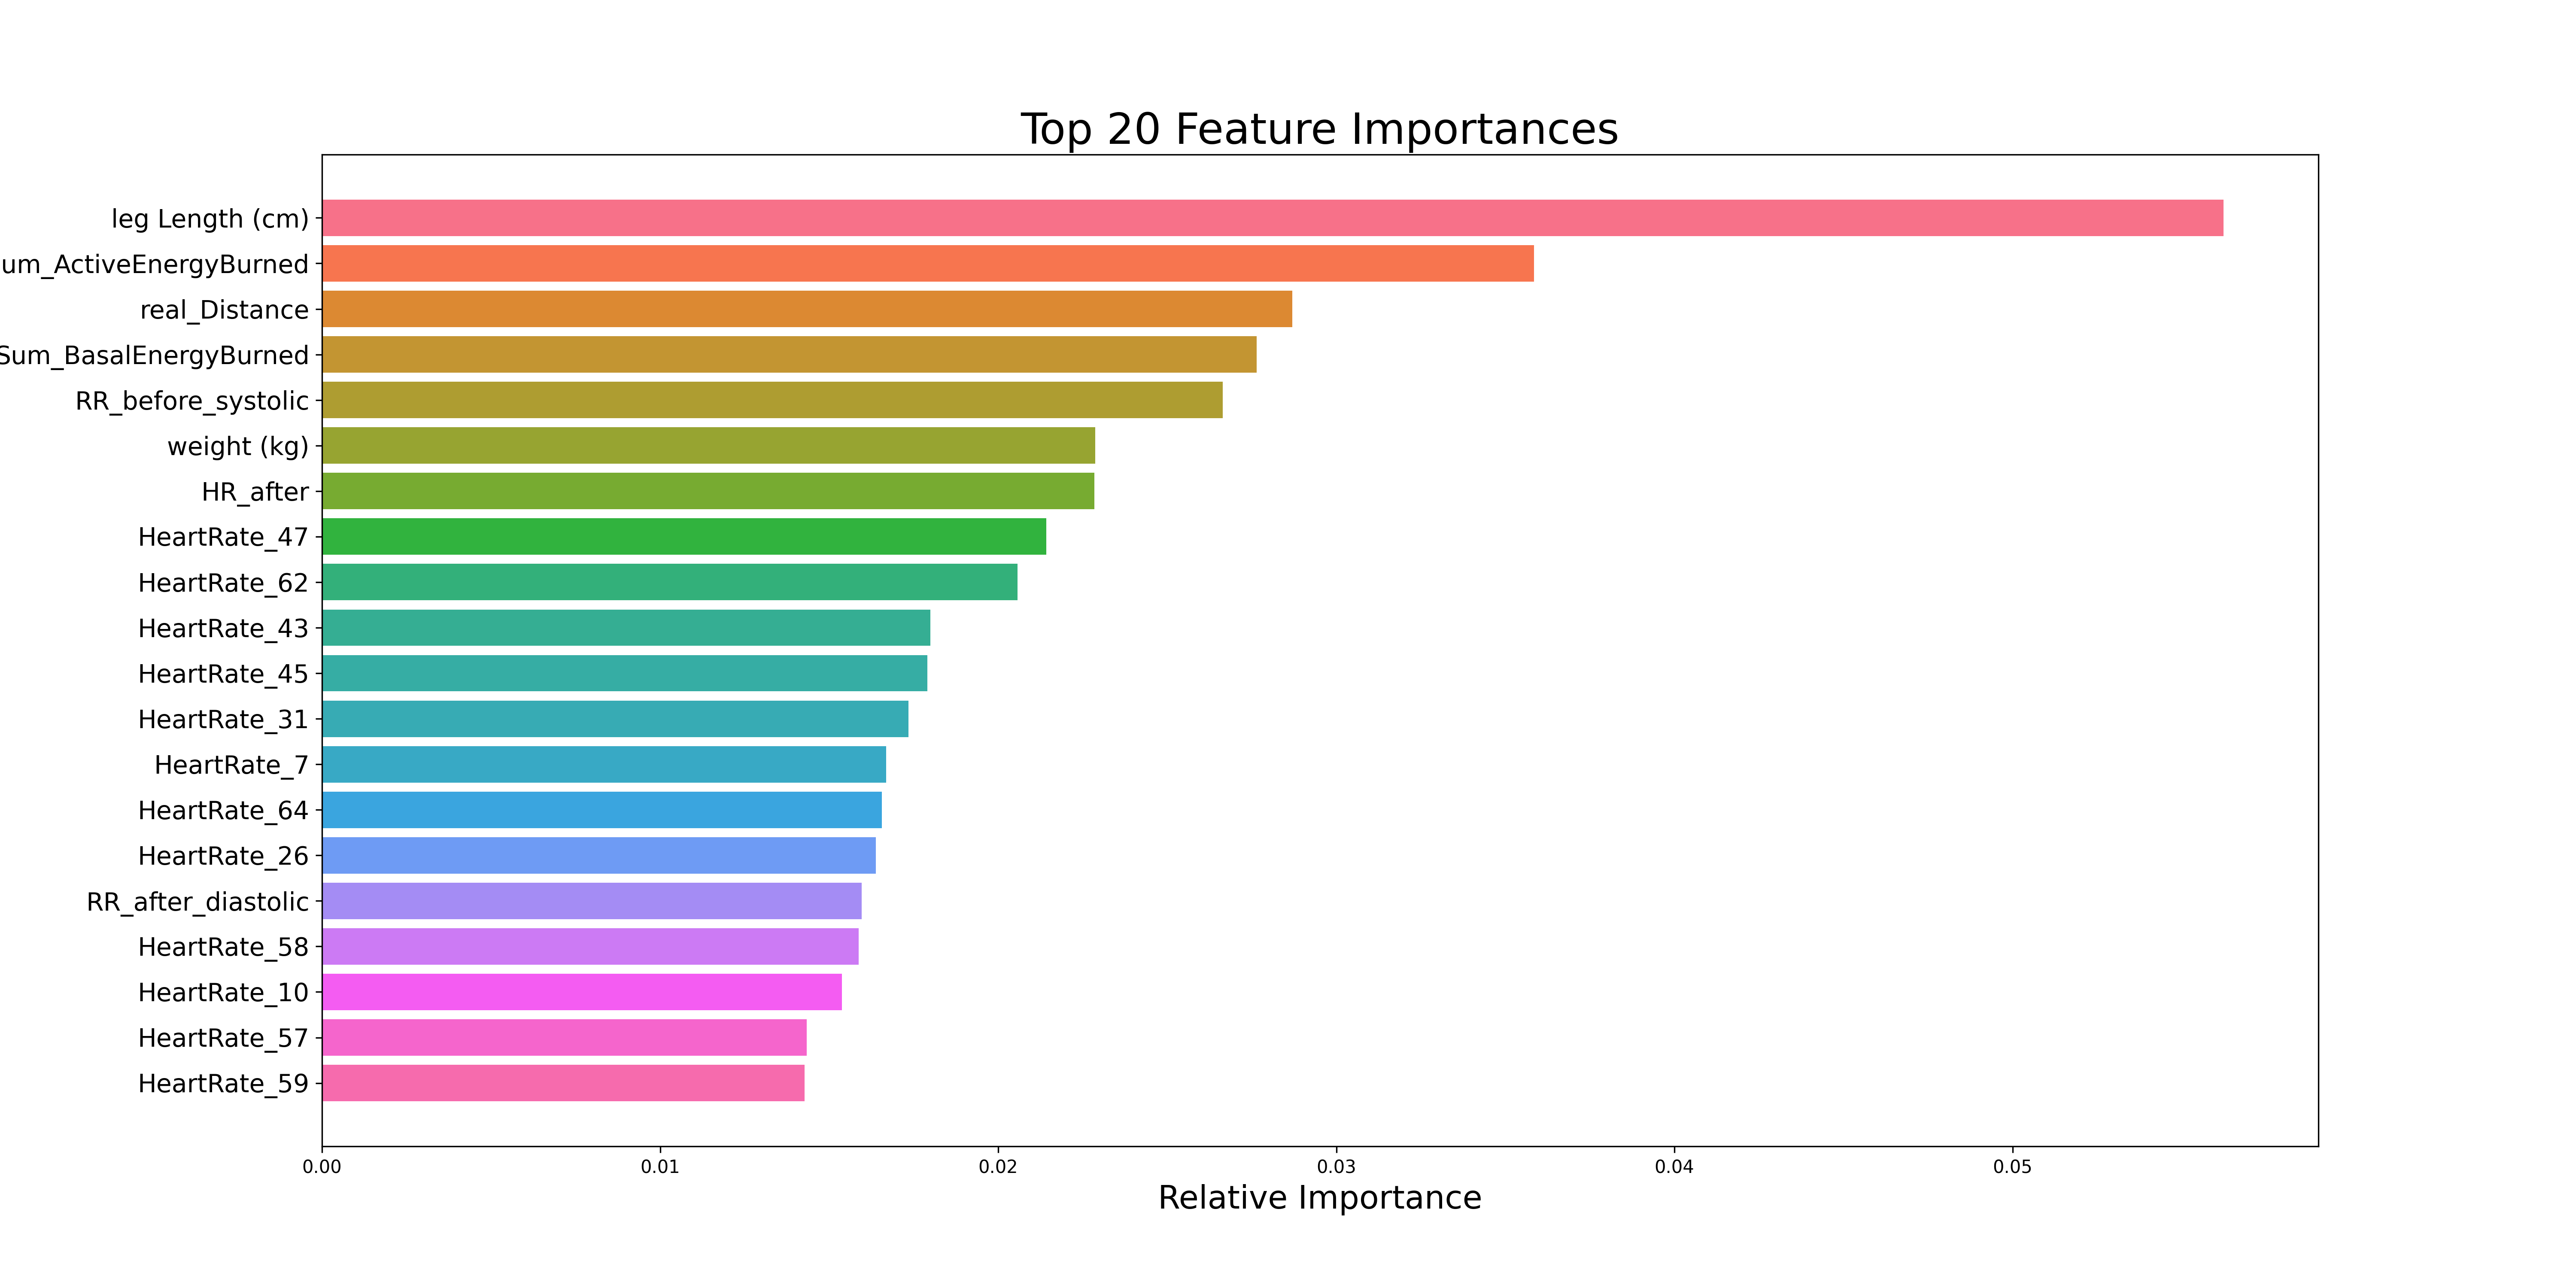
\includegraphics[width=1.0\textwidth]{Master Thesis/Plots/random_forest_top20_feature_importances_gender.png}
        \caption{Feature importance for sex prediction using RF with all given features and 100 heart rate values}
    \label{fig:featureimportanceRFsex100}
\end{figure}
\FloatBarrier

Figure ~\ref{fig:featureimportanceRFsex100} confirms the importance of height, weight, and various heart rate measurements, along with additional features like burned calories, in predicting sex. The results demonstrate the significant impact of these features on the accuracy of the RF model. And shows on the other hand that we did a prediction where the most important features where measured by the Apple Watch Ultra, what we wanted to show.

\subsubsection{Subject or Patient Classification with Random Forest}

We aimed to replicate the subject or patient prediction from chapter ~\ref{cha:results} and assess how the new features impact the results. We again started with the features the same as for table ~\ref{table:RFageHeartrate10weightheigt}, but instead of predicting sex, we predicted whether an individual is a subject or patient. Using a RF model, we achieved an accuracy of 0.83. The detailed results are as follows:

\begin{table}[H]
\centering
\begin{tabular}{lrrrr}
\toprule
{} &  precision &    recall &  f1-score &   support \\
\midrule
subject      &   0.75 &  1.00 &  0.86 &  3.0 \\
patient      &   1.00 &  0.67 &  0.80 &  3.0 \\
macro avg    &   0.88 &  0.83 &  0.83 &  6.0 \\
weighted avg &   0.88 &  0.83 &  0.83 &  6.0 \\
\bottomrule
\end{tabular}
\caption{RF subject or patient classification with all given features and 10 heart rate values}
\label{table:featureimportanceRFsubpat10}
\end{table}

The results from the RF model for predicting whether an individual is a subject or a patient are summarized in the table. The model achieved an accuracy of 0.83. The precision for predicting 'subject' is 0.75 with a recall of 1.00, resulting in an f1-score of 0.86. For predicting 'patient' the precision is 1.00 with a recall of 0.67, yielding an f1-score of 0.80. The macro average for precision, recall, and f1-score are 0.88, 0.83, and 0.83 respectively. The weighted average for all these metrics is also 0.88, 0.83, and 0.83 respectively. These results indicate a strong model performance with balanced precision and recall across both classes.

The feature importance plot provides insights into which features contributed most to the model's performance:

\FloatBarrier
\begin{figure}[h!]
    \centering
    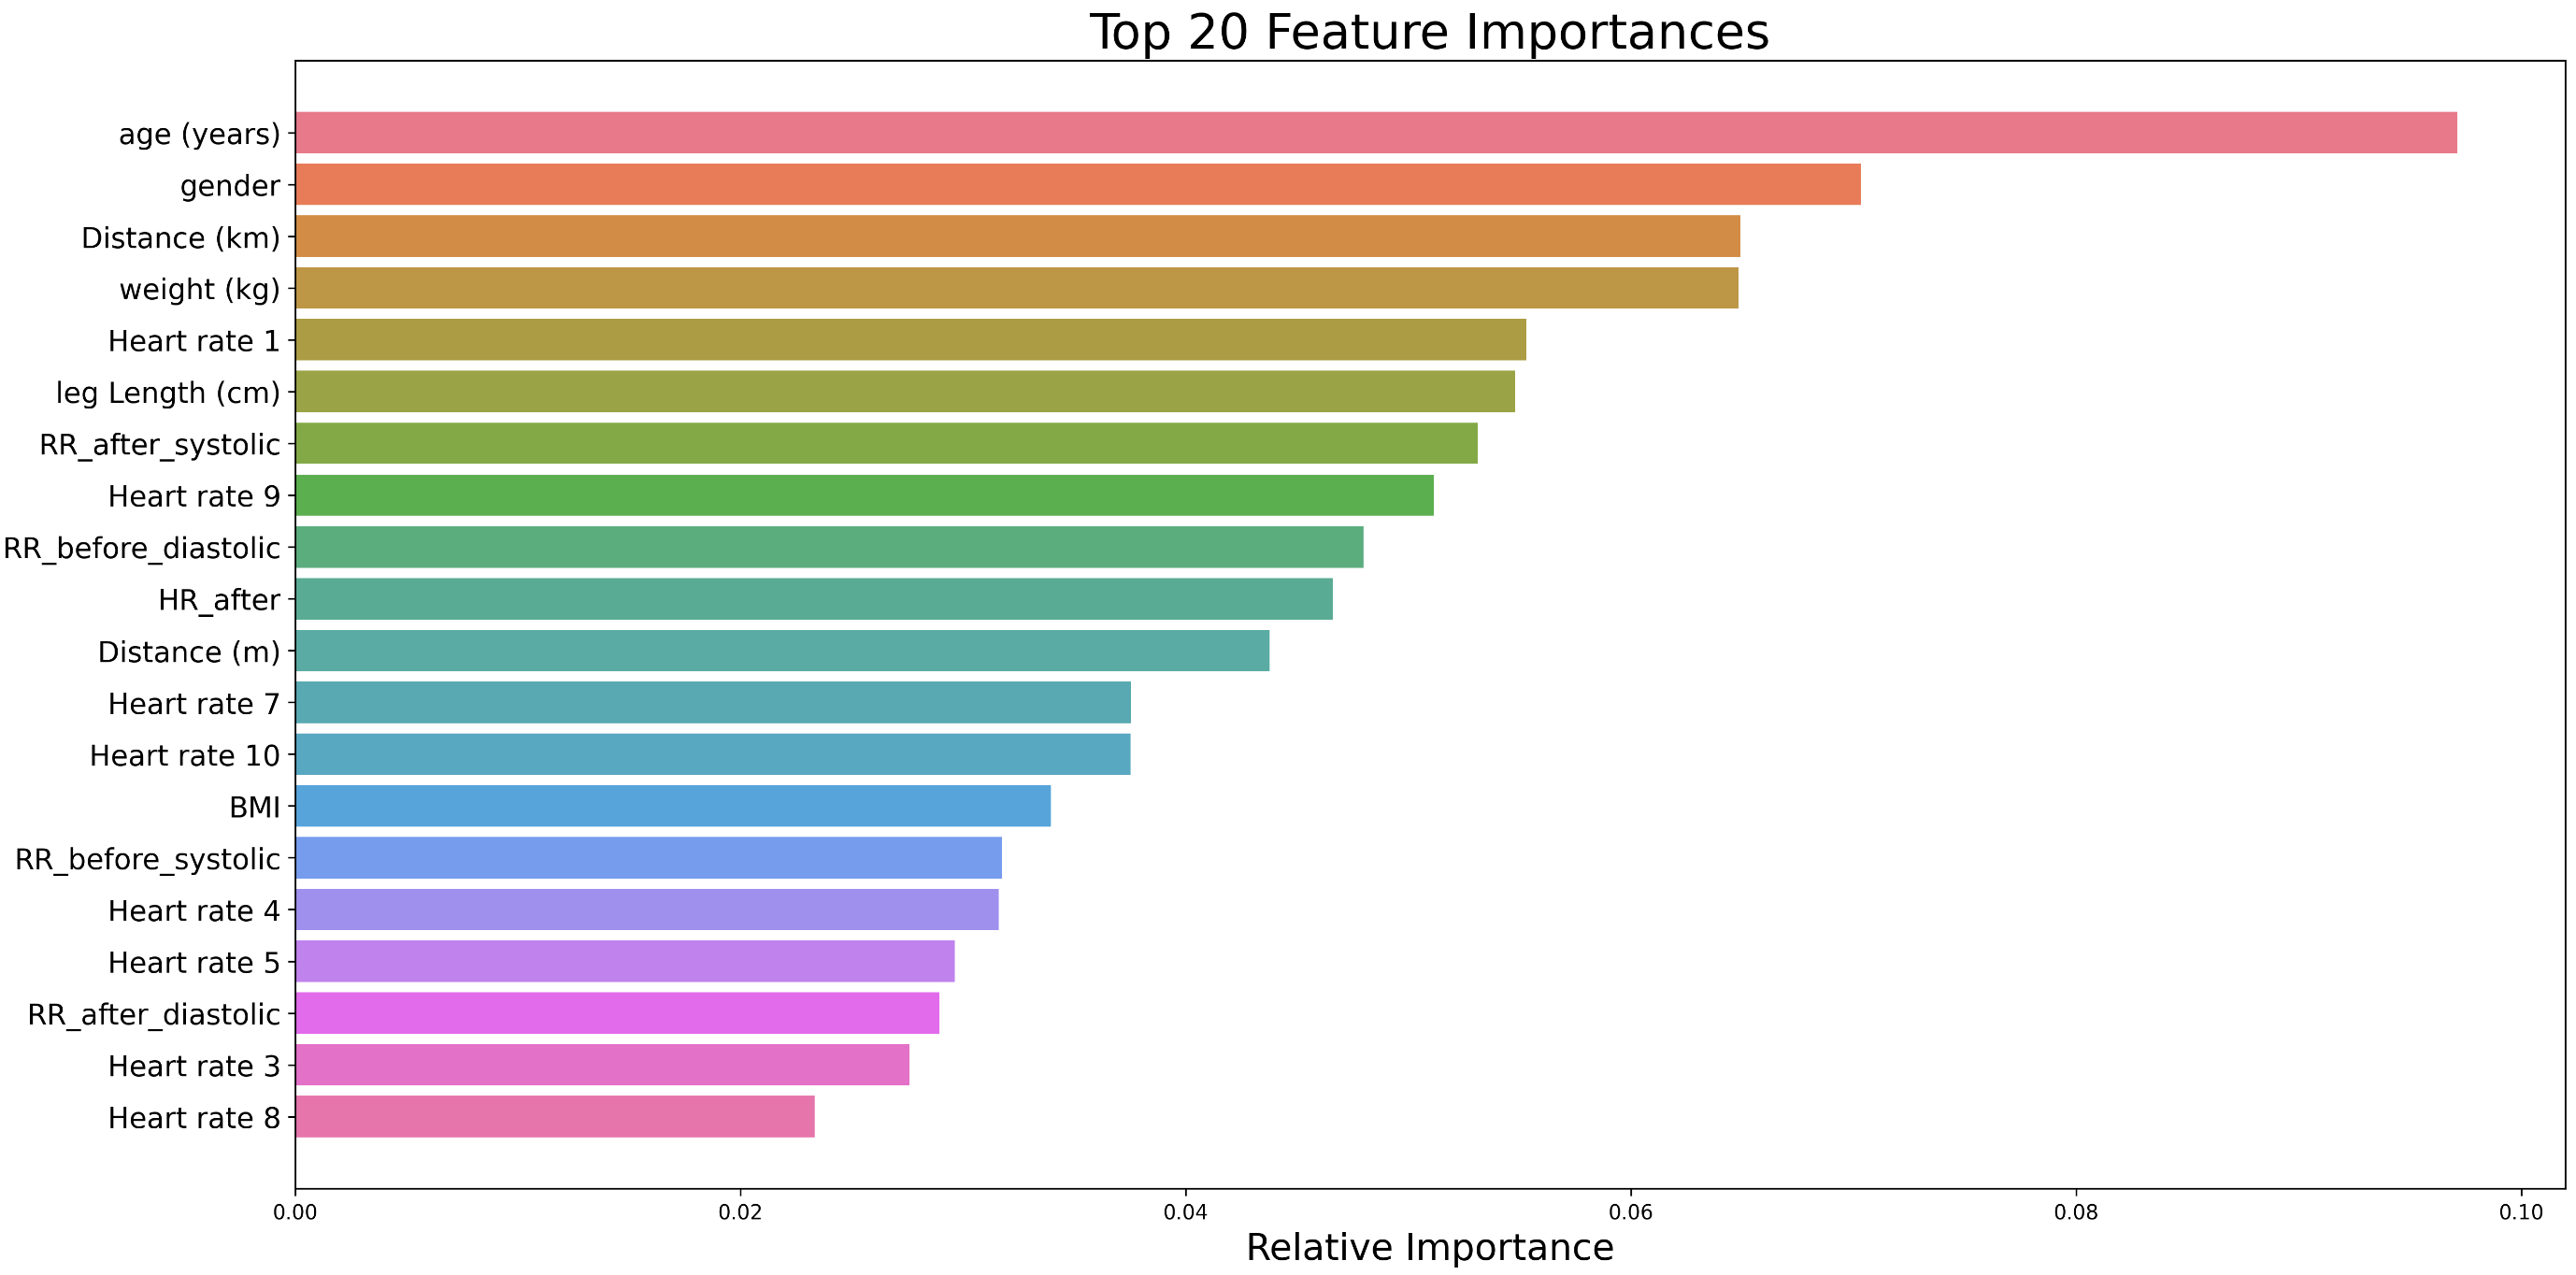
\includegraphics[width=1.0\textwidth]{Master Thesis/Plots/random_forest_top20_feature_importances_subjpatient.png}
    \caption{Feature importance for subject or patient prediction using RF with all given features and 10 heart rate values}
    \label{fig:featureimportanceRFsubpat10}
\end{figure}
\FloatBarrier

Figure ~\ref{fig:featureimportanceRFsubpat10} reveals that age, blood pressure before and after the 6MWT, and the first measured heart rate are key features for achieving a relatively accurate prediction. The importance of these features emphasizes that the Apple Watch Ultra provides relevant and important measurements that are essential for predictions.

After expanding the dataset to include the 100 heart rate measurements for each subject, sorted sequentially and added to the table, the model achieved an accuracy of 100\%, as detailed below:

\begin{table}[H]
\centering
\begin{tabular}{lrrrr}
\toprule
{} &  precision &  recall &  f1-score &  support \\
\midrule
subject            &        1.0 &     1.0 &       1.0 &      6.0 \\
patient            &        1.0 &     1.0 &       1.0 &      3.0 \\
macro avg    &        1.0 &     1.0 &       1.0 &      9.0 \\
weighted avg &        1.0 &     1.0 &       1.0 &      9.0 \\
\bottomrule
\end{tabular}
\caption{RF subject or patient classification with all given features and 100 heart rate values}
\label{table:featureimportanceRFsubpat100}
\end{table}

The classification results with the expanded dataset demonstrate exceptional performance, achieving a perfect accuracy of 100\%. Both precision and recall for each class are 1.0, indicating that the model correctly identified all instances without any errors. The macro and weighted averages also reflect perfect scores, underscoring the model's robustness and reliability in predicting the subject or patient status.

The feature importance for this model is shown in the following plot:

\FloatBarrier
\begin{figure}[h!]
    \centering
    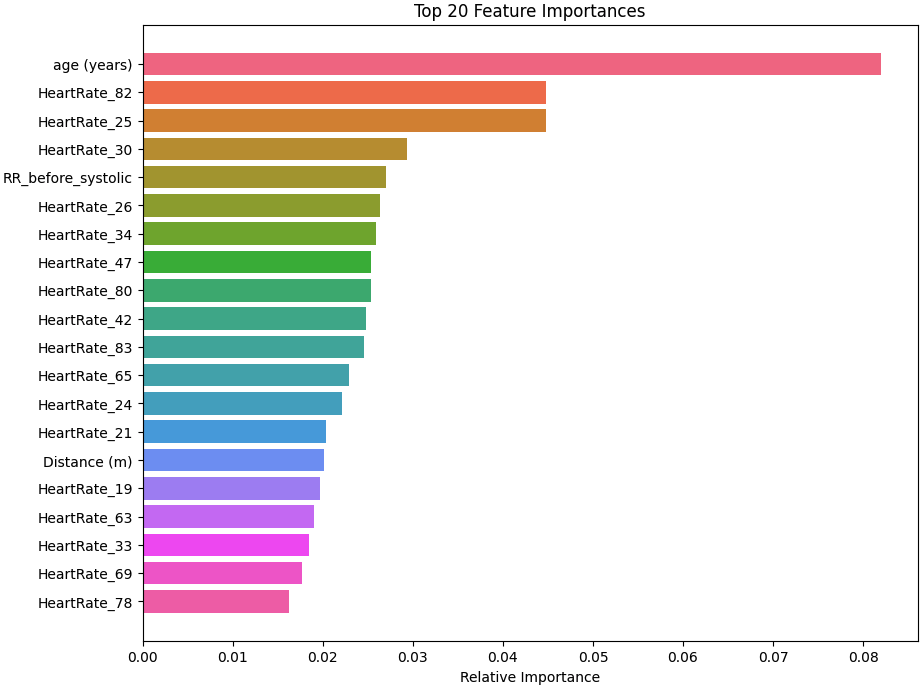
\includegraphics[width=1.0\textwidth]{Master Thesis/Plots/Random_forest_top20_patientsubject.png}
    \caption{Feature importance for subject or patient prediction using RF with all given features and 100 heart rate values}
    \label{table:featureimportanceRFsubpat100}
\end{figure}
\FloatBarrier

The feature importance figure ~\ref{table:featureimportanceRFsubpat100} shows that age is the most important factor, followed by several heart rate measurements. This emphasizes the importance of combining various features for the best prediction accuracy.

Achieving an accuracy of 100\% often means our model might be overfitting. To check this, we trained a model using only the 'age' feature, and the accuracy dropped to 88\%. This shows that age is important, but we also need other features for better predictions.

In summary, our results show that we need a full set of features for accurate predictions. While age is a strong predictor, adding other health metrics like blood pressure and heart rate improves the model. The feature importance plot below highlights the value of using different physiological and demographic factors for better accuracy. Future models will be better with larger datasets and more refined feature selection.

\subsection{Regression}

Since linear regression did not perform well with the data from chapter ~\ref{cha:results}, we decided to skip it in this chapter and directly look for optimizations or at least alternatives, hoping for better results. We started with the XGBoost model. To get a better understanding of how it compares to linear regression before applying it to our entire dataset, we first tested it on a small dataset with only a few data points.

Beside the distribution of the categories, a deeper analysis was conducted on various regression models and their outcomes. The results of the linear regression were particularly disappointing, yielding a poor RMSE value of 0.63. In contrast, the XGBoost model demonstrated significantly better performance with an RMSE value of 0.16. The generated plots are presented below:

\FloatBarrier
\begin{figure}[h]
    \centering
    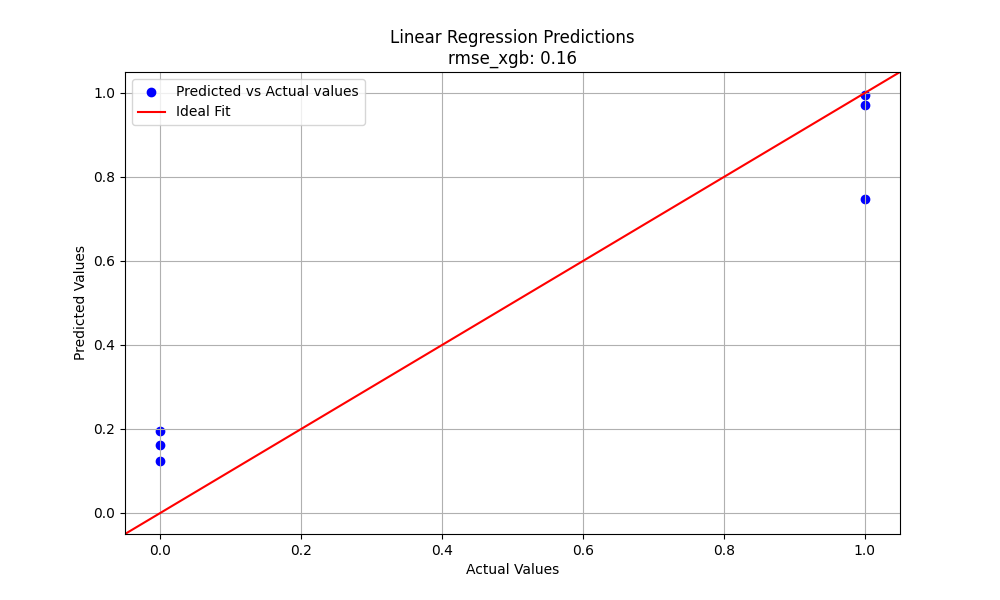
\includegraphics[width=0.75\textwidth]{Master Thesis/Plots/XG_boost_bloodPressure.png}
    \hspace{0.5cm} % Abstand zwischen den Bildern
    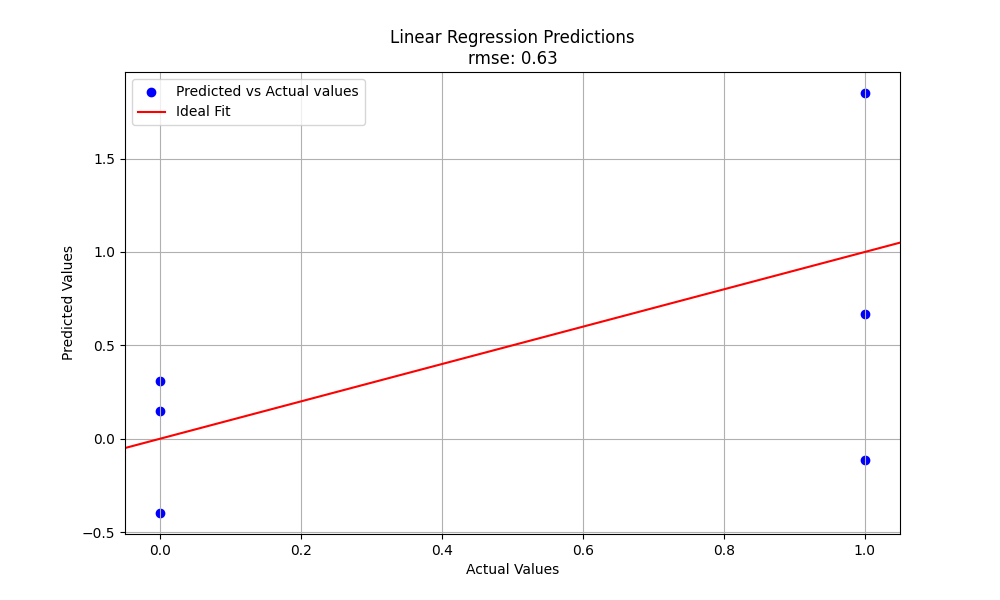
\includegraphics[width=0.75\textwidth]{Master Thesis/Plots/linReg_bloodPressure.png}
    \caption{Comparison of linear regression and XGBoost with a random part of the dataset}
    \label{fig:complinregXGBoost}
\end{figure}
\FloatBarrier

Figure ~\ref{fig:complinregXGBoost} reveals a significant difference in the performance of the two models. The XGBoost model, indicated by the plot on the top, shows blue dots clustered closely along the ideal fit line, highlighting the accuracy of the predictions. The RMSE value of 0.16 underscores the model's precision in predicting whether an individual is a subject or a patient.

On the other hand, the linear regression model, depicted in the bottom plot, shows a less favorable distribution of blue dots, which are spread farther from the ideal fit line. This is reflected in the higher RMSE value of 0.63, indicating poor predictive performance. Given that the prediction involves binary outcomes (zero and one), an RMSE of 0.63 suggests a high level of inaccuracy, making the linear regression model unreliable for this task.

In summary, the XGBoost model significantly outperforms the linear regression model, providing more accurate and reliable predictions for classifying individuals as subjects or patients based on the given features. Therefore, we will not proceed with XGBoost on our current dataset but will focus on exploring additional models to improve our predictions.

\subsubsection{Ridge Regression}
Ridge regression is particularly suitable for datasets with multicollinearity or when there are a large number of features, such as heart rate measurements in our dataset. We hoped for even better results using this regression. In the context of our study, where the dataset now consists primarily of various heart rate readings, it is essential to consider a regression model that can handle the potential collinearity among these features and provide robust predictions. Ridge regression achieves this by adding a regularization term to the loss function, which helps in managing the weights of the features effectively, preventing overfitting, and ensuring that the model remains transferable to new data. This is especially important when dealing with heart rate data, which can have many correlated variables.

Subsequently, a weighted regression analysis was performed using all measured heart rates to predict age. The results are detailed below:

\begin{table}[H]
\begin{longtable}{|>{\raggedright}p{4cm}|>{\raggedright\arraybackslash}p{10cm}|}
\hline
\textbf{metric} & \textbf{value} \\
\hline
\endfirsthead
\hline
\textbf{metric} & \textbf{value} \\
\hline
\endhead
\hline
\endfoot
ridge regression coefficients & 
\begin{minipage}[t]{10cm}
[  9.65, \   2.27, \  -5.39, \  -3.84, \   1.63, \  -2.23, \   0.25, \   6.57, \   5.23, \ -12.42, \   3.52, \  -4.34, \   8.86, \   5.17, \   0.05]
\end{minipage}
\\
\hline
ridge regression intercept & 45.33 \\
\hline
R\textsuperscript{2} on test set & 0.62 \\
\hline
MSE & 209.79 \\
\hline
RMSE & 14.48 \\
\hline
CV scores & 
\begin{minipage}[t]{10cm}
[-0.07, \ -0.56, \ -1.51, \  0.46, \ -0.34]
\end{minipage}
\\
\hline
mean CV score & -0.41 \\
\hline
\end{longtable}
\caption{Age prediction results with ridge regression based on all measured heart rates}
\label{tab:RRAgeallheart}
\end{table}

The ridge regression model for predicting age yielded a moderately good performance with an \( R^2 \) value of 0.62, explaining 62\% of the variability in the test dataset. The coefficients ranged from -12.42 to 9.65, indicating varying impacts of heart rate measurements on age prediction, with an intercept starting at 45.33. The MSE was 209.79, and the RMSE was 14.48, indicating an average prediction error of about 14.48 years. However, the CV scores ranged from -0.07 to -1.51, with a mean score of -0.41, highlighting inconsistency and potential overfitting or underfitting issues. Overall, while the model showed moderate success, its inconsistency across different subsets of data suggests the need for further refinement or alternative models.

We are satisfied with the results so far and now want to investigate the results of predicting other characteristics. The prediction of the weight with the 100 heart rate values using ridge regression provided promising results:

\begin{table}[H]
\begin{longtable}{|>{\raggedright}p{4cm}|>{\raggedright\arraybackslash}p{10cm}|}
\hline
\textbf{metric} & \textbf{value} \\
\hline
\endfirsthead
\hline
\textbf{metric} & \textbf{value} \\
\hline
\endhead
\hline
\endfoot
ridge regression coefficients & 
\begin{minipage}[t]{10cm}
[ 1.57, \  1.15, \ -0.24, \ -0.77, \  0.03, \  2.14, \  0.04, \  6.56, \  0.16, \ -0.66, \  0.49, \  4.97, \ -0.73, \  3.56, \  0.33]
\end{minipage}
\\
\hline
ridge regression intercept & 76.86 \\
\hline
ridge regression R\textsuperscript{2} on test set & 0.94 \\
\hline
MSE & 12.74 \\
\hline
RMSE & 3.57 \\
\hline
CV scores & 
\begin{minipage}[t]{10cm}
[0.59, \ 0.90, \ 0.67, \ 0.98, \ 0.87]
\end{minipage}
\\
\hline
mean CV score & 0.80 \\
\hline
\end{longtable}
\caption{Weight prediction results with ridge regression based on all measured heart rates}
\label{tab:RRweightallheart}
\end{table}

The weight prediction model performs exceptionally well, with an \( R^2 \) value of 0.94, indicating that the model explains 94\% of the variability in the test dataset. The high mean CV score of 0.80 further supports the model's robustness and reliability. The ridge regression coefficients show the importance of various features, with the intercept at 76.86. The model achieved a MSE of 12.74 and a RMSE of 3.57, demonstrating its accuracy in predicting weight.

The results of predicting BMI using ridge regression, utilizing all heart rate measurements recorded by the Apple Watch Ultra and additional non-Apple Watch Ultra data such as leg length, are detailed below:

\begin{table}[H]
\begin{longtable}{|>{\raggedright}p{4cm}|>{\raggedright\arraybackslash}p{10cm}|}
\hline
\textbf{metric} & \textbf{value} \\
\hline
\endfirsthead
\hline
\textbf{metric} & \textbf{value} \\
\hline
\endhead
\hline
\endfoot
ridge regression coefficients & 
\begin{minipage}[t]{10cm}
[ 0.56, \  0.20, \  -0.57, \ -0.07, \ -0.27, \  1.51, \  1.68, \ -0.13, \ -0.31, \  0.98, \  0.23, \ -0.37, \ -1.53, \  0.94, \ -0.31]
\end{minipage}
\\
\hline
ridge regression intercept & 25.04 \\
\hline
ridge regression R\textsuperscript{2} on test set & 0.21\\
\hline
MSE & 8.48 \\
\hline
RMSE & 2.91 \\
\hline
CV scores & 
\begin{minipage}[t]{10cm}
[0.62, \ 0.79, \ 0.84, \ 0.91, \ 0.00]
\end{minipage}
\\
\hline
mean CV score & 0.63 \\
\hline
\end{longtable}
\caption{BMI prediction results with ridge regression based on all measured heart rates}
\label{tab:RRBMIallheart}
\end{table}

The BMI prediction model demonstrates moderate performance. The ridge regression coefficients shows varying impacts of features on predicted BMI values. The ridge regression intercept is 25.04, and the \( R^2 \) value on the test set is 0.21, indicating the model explained only 21\% of the variability in the test data. The MSE is 8.48, and the RMSE is 2.91, reflecting prediction errors. CV scores ranged from 0.00 to 0.91, with a mean score of 0.63, suggesting reasonable but improvable performance. Overall, the model shows some predictive capability, but further optimization is needed.

Lastly, we attempted to predict height with all the given information, but the results were not as promising:

\begin{table}[H]
\begin{longtable}{|>{\raggedright}p{4cm}|>{\raggedright\arraybackslash}p{10cm}|}
\hline
\textbf{metric} & \textbf{value} \\
\hline
\endfirsthead
\hline
\textbf{metric} & \textbf{value} \\
\hline
\endhead
\hline
\endfoot
ridge regression coefficients & 
\begin{minipage}[t]{10cm}
[-1.09, \  0.04, \  1.75, \ -0.46, \  0.37, \  0.39, \  6.46, \  1.59, \  0.51, \ -3.72, \ -0.78, \ -1.9, \  5.77, \ -0.24, \  0.83]
\end{minipage}
\\
\hline
ridge regression intercept & 173.83 \\
\hline
ridge regression R\textsuperscript{2} on test set & -0.66\\
\hline
MSE & 105.23 \\
\hline
RMSE & 10.26 \\
\hline
CV scores & 
\begin{minipage}[t]{10cm}
[-0.13, \  0.74, \ -5.28, \  0.63, \ -0.22]
\end{minipage}
\\
\hline
mean CV score & -0.85 \\
\hline
\end{longtable}
\caption{Height prediction results with ridge regression based on all measured heart rates}
\label{tab:RRHeightallheart}
\end{table}

The height prediction model performed poorly, with an \( R^2 \) value of -0.66, indicating that the model explains very little of the variability in the test dataset. The MSE is 105.23, resulting in a RMSE of 10.26. The CV scores also varied significantly, with a mean score of -0.85, further highlighting the model's inadequacy in predicting height based on the given data.

\subsection{Weighted Linear Regression}

We decided to give linear regression another try, but given the complexity and volume of heart rate data, the standard linear regression approach wouldn't work effectively. This led us to explore weighted linear regression, a model that adjusts the influence of different data points by assigning weights, making it more suitable for datasets with varying importance among features.

We used heart rate data, along with features such as BMI, weight, and height for feature selection. We applied Principal Component Analysis (PCA) to reduce the dimensions of the heart rate data to the 10 most significant components, which we then combined with the other features. To emphasize the heart rate data, we applied weighting. We trained both linear and ridge regression models, yielding the following results:

\newpage
\begin{table}[H]
\begin{longtable}{|c|c|c|c|c|}
\hline
\textbf{feature prediction} & \textbf{metric} & \textbf{linear regression} & \textbf{ridge regression} \\
\hline
\multirow{3}{*}{weight (kg)} & R\textsuperscript{2} & 0.84 &0.99\\
& MSE & 26.66  &1.21\\
& RMSE & \textbf{5.16}  &\textbf{1.10}\\
\hline
\multirow{3}{*}{height (cm)} & R\textsuperscript{2} &  0.61 &0.98\\
& MSE & 41.14  &2.27\\
& RMSE & \textbf{6.41}  &\textbf{1.51}\\
\hline
\multirow{3}{*}{BMI} & R\textsuperscript{2} & 0.91 &0.99\\
& MSE & 0.78 &0.11\\
& RMSE & \textbf{0.88} &\textbf{0.34}\\
\hline
\multirow{3}{*}{age (years)} & R\textsuperscript{2} & 0.11 & 0.06\\
& MSE & 449.42 & 476.47\\
& RMSE & \textbf{21.20} &\textbf{21.83}\\
\hline
\multirow{3}{*}{leg length (cm)} & R\textsuperscript{2} & -0.13&0.62\\
& MSE & 63.35&21.20\\
& RMSE & \textbf{7.96} &\textbf{4.60}\\
\hline
\multirow{3}{*}{real distance (km)} & R\textsuperscript{2} & -1.22&0.72\\
& MSE & 0.02 &0.00\\
& RMSE & \textbf{0.13} &\textbf{0.05}\\
\hline
\end{longtable}
\caption{Comparison of performance metrics between linear regression and ridge regression for various prediction tasks using heart rate, BMI, weight and height features}
\label{tab:PCAallfeatures}
\end{table}


The results demonstrate significant improvement in predictive performance when using weighted heart rate values. The ridge regression model consistently outperformed linear regression, achieving higher \(R^2\) values and lower MSE and RMSE values across all features.

For weight prediction, ridge regression achieved an \(R^2\) value of 0.99, indicating almost perfect predictive power, with an RMSE of 1.10. Height prediction also saw substantial improvement with ridge regression, achieving an \(R^2\) value of 0.98 and an RMSE of 1.51.

BMI prediction performed exceptionally well, with ridge regression achieving an \(R^2\) value of 0.99 and an RMSE of 0.34. These results indicate that the model can reliably predict BMI using the available features.

Age prediction, however, did not perform as well, with an \(R^2\) value of 0.06 and an RMSE of 21.83, indicating that age prediction is challenging with the given data.

Leg length prediction showed improvement with ridge regression, achieving an \(R^2\) value of 0.62 and an RMSE of 4.60.

Real distance prediction also improved, with ridge regression achieving an \(R^2\) value of 0.72 and an RMSE of 0.05, indicating good predictive accuracy.

In summary, weighting the heart rate values and using ridge regression significantly improved the predictive power of the models for most features, except for age. This indicates that age may require additional or different features for better prediction.

\subsubsection{Experimenting with Calories Burned}

In this part of the work, we focus on analyzing and predicting the calories burned by subjects during the study. Previously, we identified that the calories burned features, measured exclusively by the Apple Watch Ultra, were highly important for our models, as shown by their feature importance rankings. Given their significance, we aim to give the calories burned features even more attention to uncover their potential further. We start with the predicting the feature of active energy burned.

\begin{table}[H]
\begin{longtable}{|>{\raggedright}p{4cm}|>{\raggedright\arraybackslash}p{10cm}|}
\hline
\textbf{metric} & \textbf{value} \\
\hline
\endfirsthead
\hline
\textbf{metric} & \textbf{value} \\
\hline
\endhead
\hline
\endfoot
MSE & 26.47 \\
\hline
RMSE & 5.14 \\
\hline
R\textsuperscript{2} score & 0.76 \\
\hline
CV scores &
\begin{minipage}[t]{10cm}
[-0.40, \ 0.79, \ 0.47, \ -1.25, \ -0.49]
\end{minipage}
\\
\hline
mean CV score & -0.18 \\
\hline
\end{longtable}
\caption{Active energy burned prediction results with ridge regression based on all measured values}
\label{tab:RRcaloriesallfeatures}
\end{table}

The analysis of the MSE reveals a value of 26.47, indicating a notable discrepancy between the predicted and actual values. Although not excessively high, this discrepancy suggests there is room for improvement in the model's accuracy. The RMSE of 5.14 further quantifies the average prediction error in the same units as the target variable, highlighting the extent to which the model's predictions deviate from actual measurements.

An R\textsuperscript{2} score of 0.76 suggests that 76\% of the variability in active energy burned can be explained by the features included in the model. This relatively high R\textsuperscript{2} score indicates that the model captures a substantial portion of the underlying patterns in the data. However, 24\% of the variability remains unexplained, likely due to factors not included in the model.

The CV scores, which range from -1.25 to 0.79, highlight inconsistencies in the model's performance across different subsets of the data. The presence of negative CV scores indicates that, for certain data folds, the model performs worse than a simple baseline model that predicts the mean value. The mean CV score of -0.18 underscores this inconsistency, suggesting that the model does not generalize well across all data partitions and might be overfitting to certain subsets.

To visualize the significance of the various features, we will present a plot of the top 20 most important features for predicting active energy burned, providing a clearer understanding of their impact on the model's performance:

\FloatBarrier
\begin{figure}[h!]
    \centering
    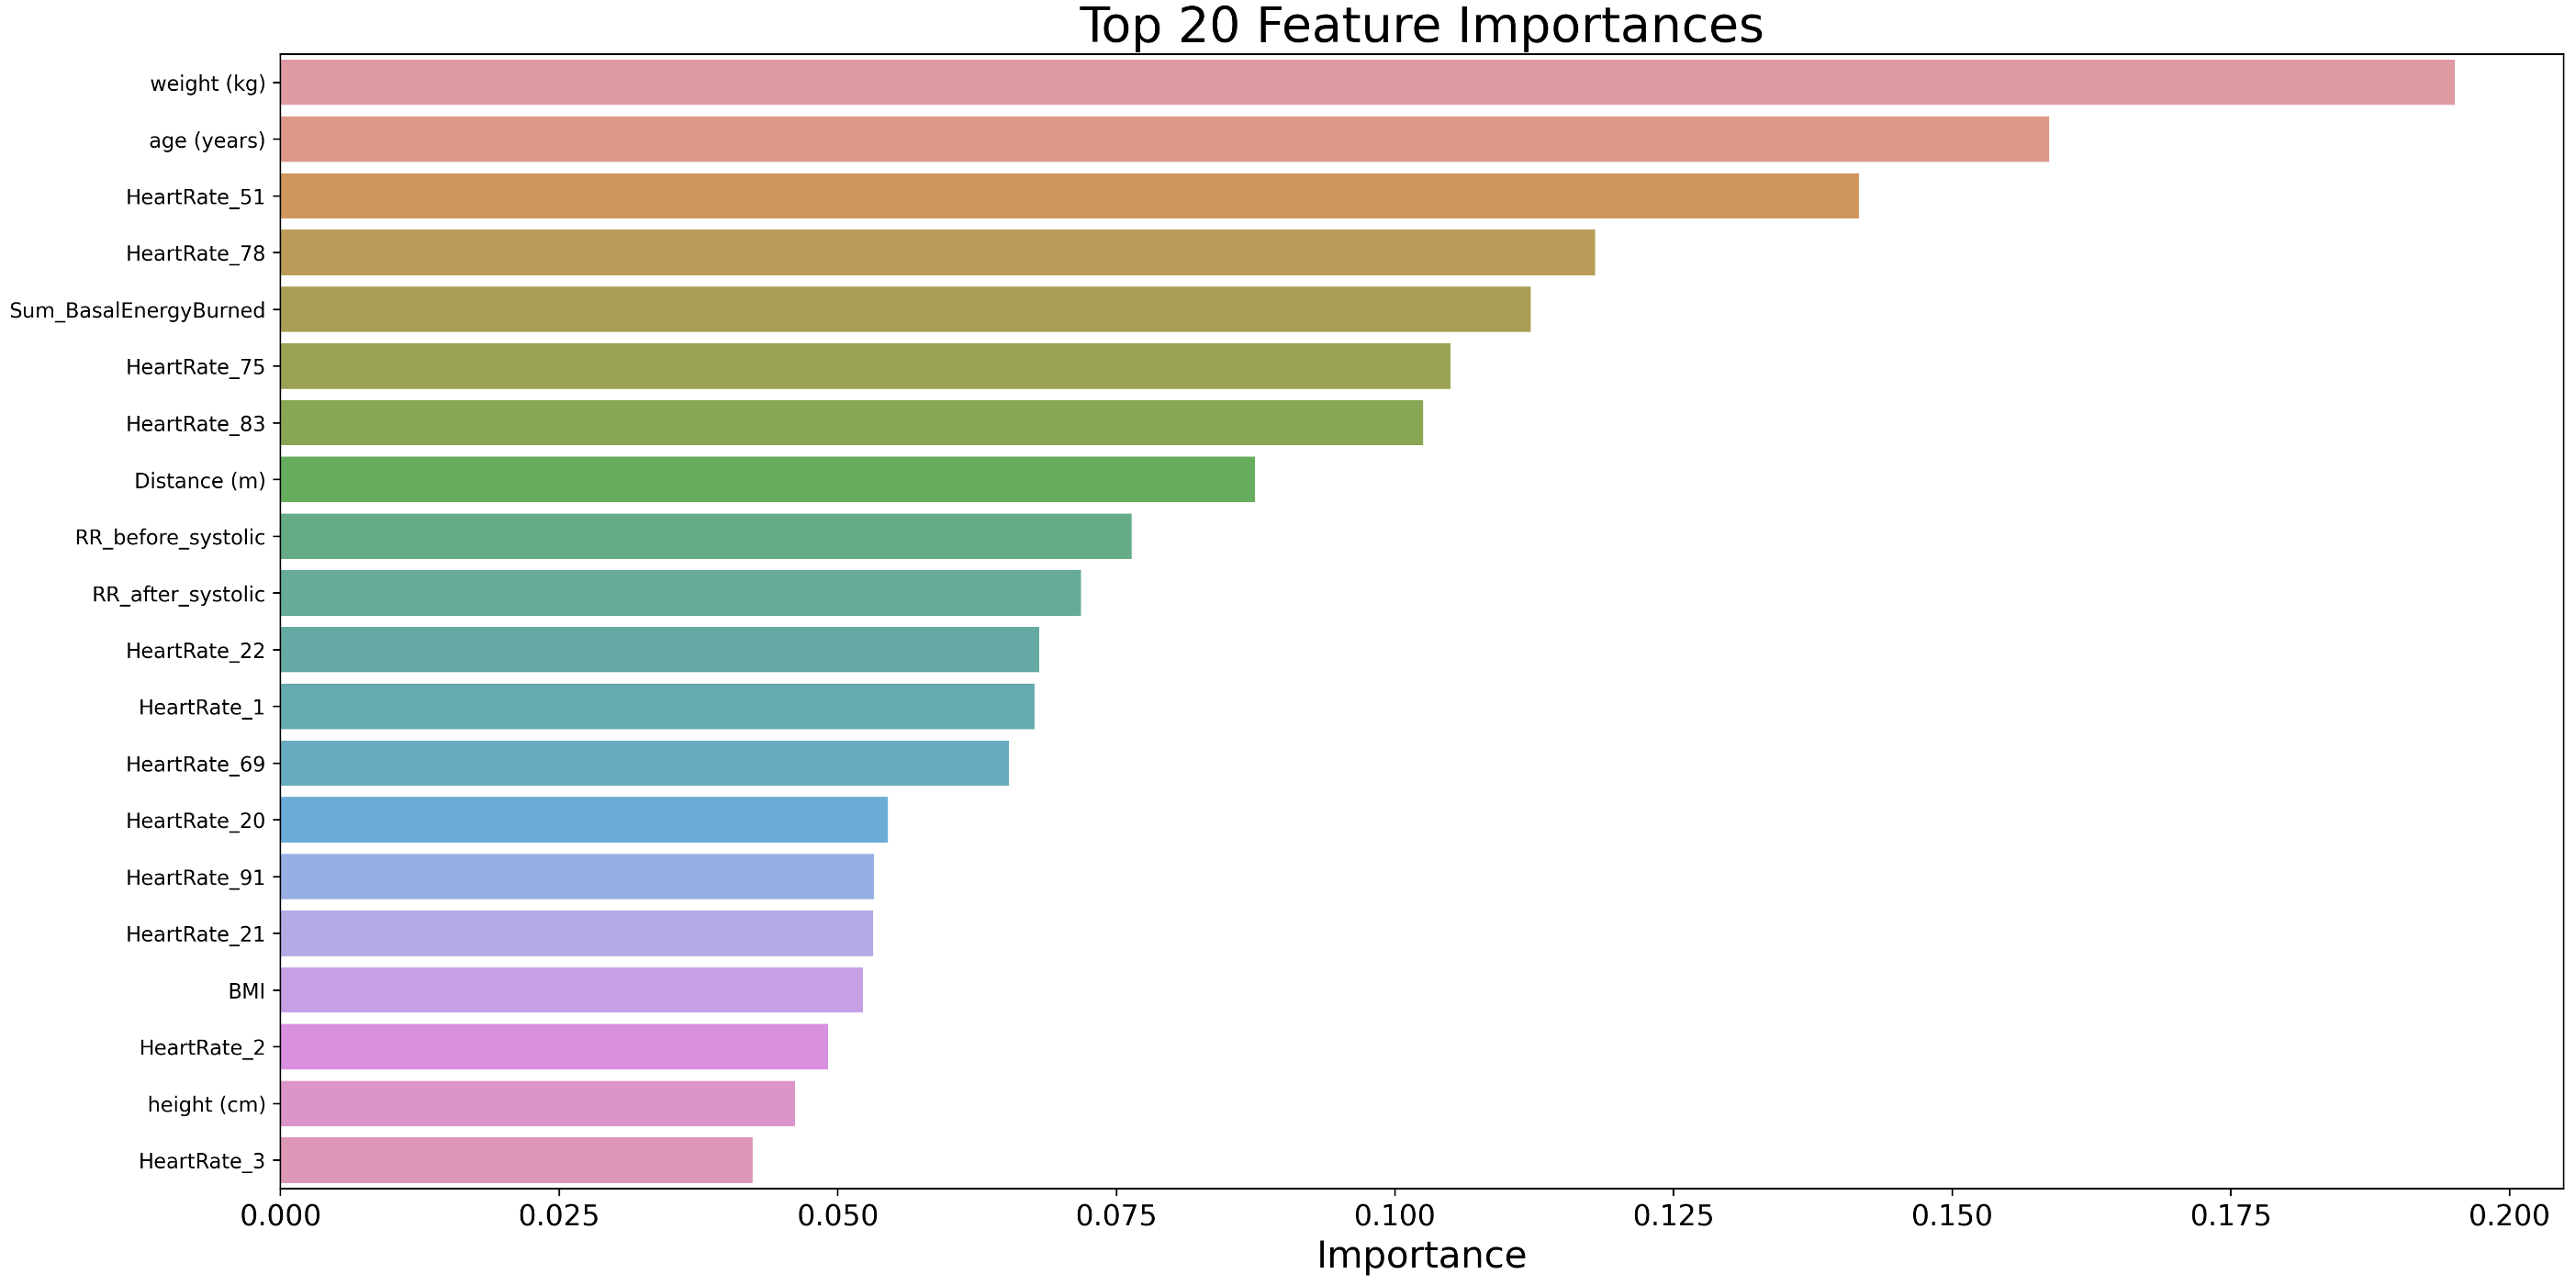
\includegraphics[width=1.0\textwidth]{Master Thesis/Plots/Top_20_Importance_activeEnergy2.png}
        \caption{Feature importance for active energy burned prediction using ridge regression with all given features}
    \label{fig:featureimportanceRRallact}
\end{figure}
\FloatBarrier

Figure ~\ref{fig:featureimportanceRRallact} identifies the top 20 features that the model relies on for predicting active energy burned. The feature weight (kg) emerges as the most critical feature, indicating its significant influence on the model's predictions. The feature age (years) is another key factor, reflecting the impact of age-related metabolic changes on energy expenditure. Various heart rate measurements also play a crucial role, underscoring the importance of the Apple Watch Ultra data in predicting active energy expenditure. Additionally, the basal energy burned feature is highlighted, indicating its strong correlation with active energy burned which is measured by the watch as well. The distance covered by subjects is also a notable predictor, emphasizing the relationship between physical activity and calorie expenditure. Blood pressure measurements before and after the exercise session further contribute to the model's predictions, suggesting the relevance of cardiovascular health metrics.

Continuing our analysis, we focused on predicting basal energy burned, which represents the calories expended at rest to maintain vital bodily functions. The following results detail the model's performance in predicting basal energy burned:

\begin{table}[H]
\begin{longtable}{|>{\raggedright}p{4cm}|>{\raggedright\arraybackslash}p{10cm}|}
\hline
\textbf{metric} & \textbf{value} \\
\hline
\endfirsthead
\hline
\textbf{metric} & \textbf{value} \\
\hline
\endhead
\hline
\endfoot
MSE & 95.17 \\
\hline
RMSE & 9.76 \\
\hline
R\textsuperscript{2} score & 0.21 \\
\hline
CV Scores &
\begin{minipage}[t]{10cm}
[0.23, \ 0.43, \ -0.14, \ -1.04, \ -0.07]
\end{minipage}
\\
\hline
mean CV score & -0.12 \\
\hline
\end{longtable}
\caption{Basal energy burned prediction results with ridge regression based on all measured values}
\label{tab:RRcbasalaloriesallfeatures}
\end{table}

The evaluation of the MSE yielded a value of 95.17, indicating a substantial gap between the predicted and actual basal energy burned values. The RMSE of 9.76 further supports this finding, reflecting the average magnitude of error in the same units as the target variable. These errors suggest that the model's predictions are not highly accurate.

An R\textsuperscript{2} score of 0.21 indicates that only 21\% of the variance in basal energy burned is explained by the features in the model, pointing to a relatively weak explanatory power. This low R\textsuperscript{2} score suggests that there are other factors affecting basal energy burned that are not captured by the model.

The CV scores, ranging from -1.04 to 0.43, reveal variability in the model's performance across different subsets of the data. The presence of negative CV scores for some folds indicates that, in certain cases, the model performs worse than a simple baseline model. The mean CV score of -0.12 further underscores the inconsistency and potential overfitting of the model to specific subsets of the data.

To visualize the significance of the various features, we will present a plot of the top 20 most important features for predicting basal energy burned, providing a clearer understanding of their impact on the model's performance:

\FloatBarrier
\begin{figure}[h!]
    \centering
    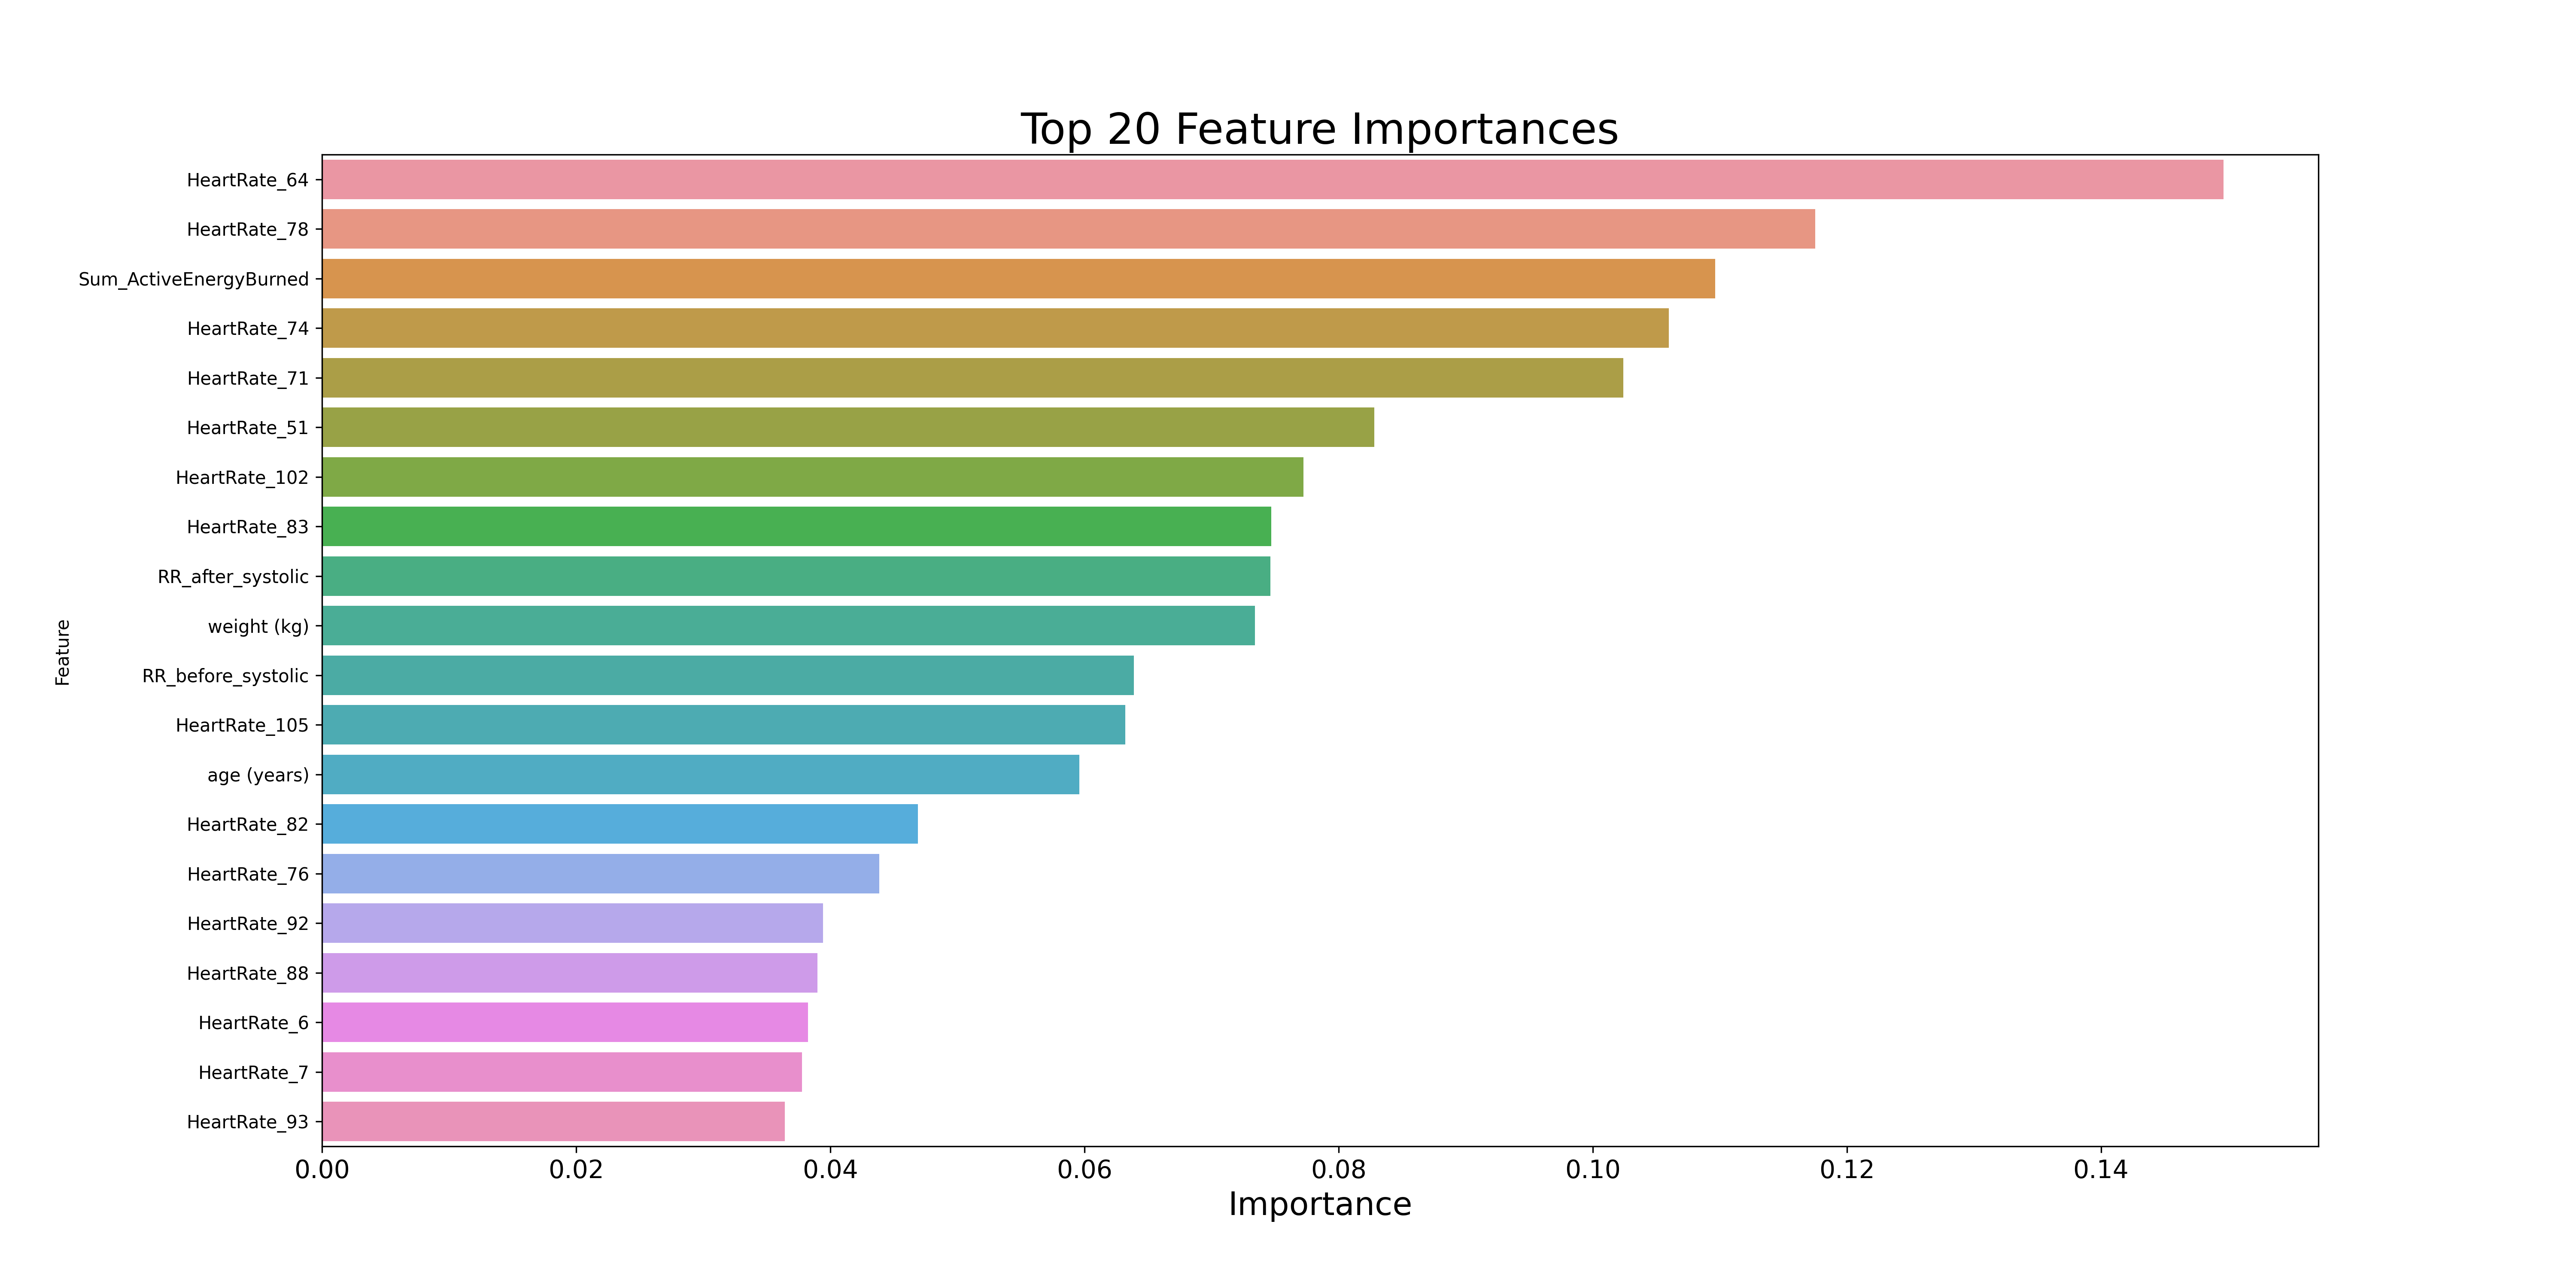
\includegraphics[width=1.0\textwidth]{Master Thesis/Plots/Top_20_Importance_basalEnergy.png}
      \caption{Feature importance for basal energy burned prediction using ridge regression with all given features}
    \label{fig:featureimportanceRRallbas}
\end{figure}
\FloatBarrier

Figure ~\ref{fig:featureimportanceRRallbas} highlights the top 20 features utilized by the model for predicting basal energy burned. Heart rate measurements dominate the list, with 'HeartRate\_64', 'HeartRate\_78', and 'Sum\_ActiveEnergyBurned' being the most influential features. This underscores the critical role of heart rate data in estimating basal energy expenditure. Additional heart rate values, both systolic and diastolic blood pressure measurements, and weight are also significant contributors. The diversity of important features suggests that basal energy burned is influenced by a combination of cardiovascular metrics, body measurements, and overall physical activity.

In summary, while the model demonstrates some capacity to predict basal energy burned, its limited accuracy highlights the need for further refinement and possibly additional features to improve performance.

\subsection{Neural Networks}

We decided to use our new dataset, which has many heart rate measurements and other, not Apple Watch Ultra recorded data, to try NNs again. We hope that these different and additional features will lead to better results. We used all received data in this subsection.

The NN we used has several dense and dropout layers.

The architecture includes:
\begin{itemize}
    \item A dense layer with 256 neurons, ReLU activation, and L2 regularization (0.01)
    \item A dropout layer with a 40\% rate 
    \item Another dense layer with 128 neurons, ReLU activation, and L2 regularization (0.01)
    \item A dropout layer with a 30\% rate
    \item A dense layer with 64 neurons, ReLU activation, and L2 regularization (0.01)
    \item An output layer with 1 neuron
\end{itemize}

The model was compiled using the Adam optimizer and the MSE loss function. Training was conducted for 3000 epochs with a batch size of 32. 

With all these settings we have achieved the following results:

\newpage
\begin{table}[H]
\begin{longtable}{|c|c|c|c|c|}
\hline
\textbf{feature} & \textbf{metric} & \textbf{PCA (n=10)} & \textbf{PCA (n=15)} & \textbf{PCA (n=20)} \\
\hline
\multirow{3}{*}{weight (kg)} & R\textsuperscript{2} & & -15.75 & \\
& MSE & & 13.50 & \\
& RMSE & & \textbf{3.67} & \\
\hline
\multirow{3}{*}{height (cm)} & R\textsuperscript{2} & & -56.58 & \\
& MSE & & 53.39 & \\
& RMSE & & \textbf{7.31} & \\
\hline
\multirow{3}{*}{BMI} & R\textsuperscript{2} & & -1.48 & \\
& MSE & & 0.57 & \\
& RMSE & & \textbf{0.75} & \\
\hline
\multirow{3}{*}{age (years)} & R\textsuperscript{2} & -314.44 & -317.00 & -335.47 \\
& MSE & 311.99 & 314.60 & 333.02 \\
& RMSE & \textbf{17.66} & \textbf{17.74} & \textbf{18.25} \\
\hline
\multirow{3}{*}{leg length (cm)} & R\textsuperscript{2} & -47.17 & -47.59 & \\
& MSE & 44.85 & 45.30 & \\
& RMSE & \textbf{6.70} & \textbf{6.73} & \\
\hline
\multirow{3}{*}{real distance (km)} & R\textsuperscript{2} & & -0.006 & \\
& MSE & & 0.002 & \\
& RMSE & & \textbf{0.047} & \\
\hline
\multirow{3}{*}{BMI over 25} & R\textsuperscript{2} & & -0.03 & \\
& MSE & & 0.01 & \\
& RMSE & & \textbf{0.11} & \\
\hline
\multirow{3}{*}{subject/patient} & R\textsuperscript{2} & & -0.06 & -0.04 \\
& MSE & & 0.04 & 0.02 \\
& RMSE & & \textbf{0.20} & \textbf{0.15} \\
\hline
\end{longtable}
\caption{Comparison of performance between NNs with different PCA setting for various prediction tasks using all features}
\label{tab:PCAdiffallfeatures}
\end{table}

The results for the NN models with different PCA configurations shows mixed performance. Most features have negative R\textsuperscript{2} values, indicating that the models perform worse than a simple mean prediction. This suggests that the models fail to explain the variability of the target variables effectively. Despite the poor R\textsuperscript{2} values, the RMSE values are relatively reasonable. For instance, the RMSE for predicting real distance is 0.047, indicating an average prediction error of 47 meters. However, this may be misleading because the walking distances of most participants are similar, which reduces variability and artificially improves RMSE.

In summary, the negative R\textsuperscript{2} values highlight the poor performance of the models in predicting the target variables, suggesting that the models are not capturing the underlying patterns effectively. While the RMSE values appear reasonable, they might not fully reflect the model's predictive power due to low variability in the dataset. To address these issues, further refinement is necessary to improve the model performance.

\newpage
To enhance the results, we developed a new NN model with a reduced number of PCA components and an optimized architecture tailored for binary classification problems. We first did the subject or patient prediction with all the given data and all features but without the weight. We made adjustments to the loss function and activation function of the output layer and included a validation split to monitor performance. The results are detailed below:

\begin{table}[H]
\begin{longtable}{|>{\raggedright}p{4cm}|>{\raggedright\arraybackslash}p{10cm}|}
\hline
\textbf{metric} & \textbf{value} \\
\hline
\endfirsthead
\hline
\textbf{metric} & \textbf{value} \\
\hline
\endhead
\hline
\endfoot
NN R\textsuperscript{2} on test set (accuracy) & 1.0 \\
\hline
MSE on test set & 0.0 \\
\hline
RMSE on test set & 0.0 \\
\hline
\end{longtable}
\caption{Performance of NN after loss function adjustment using all features for subject or patient prediction}
\label{tab:PCAdiffallfeatures}
\end{table}

The NN achieved an R\textsuperscript{2} value of 1.0 on the test set, indicating perfect predictive performance. Both the MSE and RMSE are 0.0, which further supports the model's accuracy in making predictions. These values suggest that the model is highly precise and has no error in its predictions of a subject or patient for the test set.

The following plots illustrate the accuracy and loss during the training process, offering additional insights into the model's learning dynamics and potential areas for further optimization:

\FloatBarrier
\begin{figure}[h!]
    \centering
    \includegraphics[width=1.0\textwidth]{Master Thesis/Plots/DL_all_Acc.png}
    \caption{Accuracy of deep learning model with extended dataset for subject or patient prediction}
\label{figure:modelaccNNalldata}
\end{figure}
\FloatBarrier

\FloatBarrier
\begin{figure}[h!]
\centering
    \includegraphics[width=1.0\textwidth]{Master Thesis/Plots/DL_all_Loss.png}
    \caption{Loss of deep learning model with extended dataset for subject or patient prediction}
\label{figure:modellossNNalldat}
\end{figure}
\FloatBarrier

The accuracy plot (Figure ~\ref{figure:modelaccNNalldata}) depicts the model's performance on the training and validation sets across epochs. The training accuracy exhibits significant fluctuations, indicating instability during the learning process. On the other hand, the validation accuracy remains relatively stable but consistently lower than the training accuracy, suggesting that the model struggles to generalize well to new data.

The loss plot (Figure ~\ref{figure:modellossNNalldat}) shows the progression of the loss function over epochs. The training loss decreases steadily, indicating that the model is learning from the data. However, the validation loss is notably higher and increases over time, reinforcing the indication of overfitting. This suggests that while the model is improving its performance on the training set, it does not perform as well on the validation set.

Before we draw a final conclusion on the performance of NN and other ML methods evaluated in this thesis, we aimed to extend our analysis to include risk prediction. Similar to our previous models, we focused on predicting whether a subject has a BMI over 25, which we had classified as a risk factor. This additional analysis provided further insights into the applicability and effectiveness of our models in predicting health-related risks. We achieved following results:

\begin{table}[H]
\begin{longtable}{|>{\raggedright}p{4cm}|>{\raggedright\arraybackslash}p{10cm}|}
\hline
\textbf{metric} & \textbf{value} \\
\hline
\endfirsthead
\hline
\textbf{metric} & \textbf{value} \\
\hline
\endhead
\hline
\endfoot
NN R\textsuperscript{2} on test set (accuracy) & 0.78 \\
\hline
MSE on test set & 0.23 \\
\hline
RMSE on test set & 0.47 \\
\hline
\end{longtable}
\caption{Performance of NN after loss function adjustment using all features for risk prediction}
\label{tab:PCAdiffallfeaturesrisk}
\end{table}

The R\textsuperscript{2} value of 0.78 indicates that the neural network explains 78\% of the variance in the risk prediction task. This is a strong performance, suggesting that the model is fairly accurate in predicting whether a subject has a BMI over 25.

The MSE of 0.23 reflects the average squared difference between the predicted and actual values. While not perfect, this relatively low MSE indicates that the predictions are generally close to the actual outcomes.

The RMSE of 0.47 further quantifies the model's prediction error, providing a more interpretable metric since it is on the same scale as the original values. An RMSE of 0.47 suggests that the model's predictions deviate from the actual values by an average of 0.47 units.

These metrics demonstrate that the NN performs well in the risk prediction task, with a strong R\textsuperscript{2} value and relatively low MSE and RMSE. However, there is still room for improvement.

The following plots illustrate the NNs performance during the risk prediction task, showing the training and validation loss, as well as accuracy over 3000 epochs:

\FloatBarrier
\begin{figure}[h!]
\centering
    \includegraphics[width=1.0\textwidth]{Master Thesis/Plots/NN_all_risk_loss.png}
    \caption{Accuracy of deep learning model with extended dataset for risk prediction}
\label{figure:modellossNNalldatriskacc}
\end{figure}
\FloatBarrier

\FloatBarrier
\begin{figure}[h!]
    \centering
    \includegraphics[width=1.0\textwidth]{Master Thesis/Plots/NN_all_risk_acc.png}
    \caption{Loss of deep learning model with extended dataset for risk prediction}
\label{figure:modelaccNNalldatariskloss}
\end{figure}
\FloatBarrier

The accuracy plot (Figure ~\ref{figure:modellossNNalldatriskacc}) demonstrates that the training accuracy (blue line) reaches nearly 1.0 quickly, showing near-perfect performance on the training set. In contrast, the validation accuracy (orange line) remains lower and fluctuates around 0.75, confirming overfitting.

The loss function plot (Figure ~\ref{figure:modelaccNNalldatariskloss}) shows that the training loss (blue line) decreases quickly and stays low, indicating effective learning from the training data. However, the validation loss (orange line) is much higher and fluctuates significantly, indicating overfitting and instability on new data.

These two plots reveal that while the neural network performs well on the training set, it overfits and does not generalize well to the validation set.

In conclusion, while the model shows potential with the comprehensive set of features, it is crucial to address overfitting to ensure robust performance on unseen data. 

Given the nature of our dataset and the specific prediction tasks, we opted not to use unsupervised learning models for this analysis and move directly to the final conclusion, as we do not anticipate better results than those discussed in chapter ~\ref{cha:results}.

\newpage
\section{Summary Table of Chapter Results}
\FloatBarrier
\notsotiny
\begin{longtable}{llrrrrr}
    \caption{Summary of all results in chapter 8 for various models and feature sets} \\
    \toprule
    \textbf{prediction task} & \textbf{features / metrics} & \textbf{precision} & \textbf{recall} & \textbf{f1-score} & \textbf{support} & \textbf{accuracy} \\
    \midrule
    \endfirsthead
    \caption[]{Summary of all results in chapter 8 for various models and feature sets (continued)} \\
    \toprule
    \textbf{prediction task} & \textbf{features} & \textbf{precision} & \textbf{recall} & \textbf{f1-score} & \textbf{support} & \textbf{accuracy} \\
    \midrule
    \endhead
    \bottomrule
    \endfoot
    \multirow{6}{*}{sex prediction (RF)} 
    & age, height, weight, heart rates, blood pressure & & & & & 1.00 \\
    & female & 1.00 & 1.00 & 1.00 & 2.00 & \\
    & male & 1.00 & 1.00 & 1.00 & 4.00 & \\
    & macro avg & 1.00 & 1.00 & 1.00 & 6.00 & \\
    & weighted avg & 1.00 & 1.00 & 1.00 & 6.00 & \\
    \midrule
    \multirow{6}{*}{sex prediction (RF)} 
    & age, height, weight, 100 heart rate values & & & & & 0.78 \\
    & female & 0.71 & 1.00 & 0.83 & 5.0 & \\
    & male & 1.00 & 0.50 & 0.67 & 4.0 & \\
    & macro avg & 0.86 & 0.75 & 0.75 & 9.0 & \\
    & weighted avg & 0.84 & 0.78 & 0.76 & 9.0 & \\
    \midrule
    \multirow{6}{*}{subject/patient prediction (RF)} 
    & age, height, weight, heart rates, blood pressure & & & & & 0.83 \\
    & subject & 0.75 & 1.00 & 0.86 & 3.0 & \\
    & patient & 1.00 & 0.67 & 0.80 & 3.0 & \\
    & macro avg & 0.88 & 0.83 & 0.83 & 6.0 & \\
    & weighted avg & 0.88 & 0.83 & 0.83 & 6.0 & \\
    \midrule
    \multirow{7}{*}{subject/patient prediction (RF)} 
    & age, height, weight, blood pressure and & & & & & 1.00 \\
    & 100 heart rate values & & & & &  \\
    & subject & 1.00 & 1.00 & 1.00 & 6.0 & \\
    & patient & 1.00 & 1.00 & 1.00 & 3.0 & \\
    & macro avg & 1.00 & 1.00 & 1.00 & 9.0 & \\
    & weighted avg & 1.00 & 1.00 & 1.00 & 9.0 & \\
    \midrule
    \multirow{6}{*}{ridge regression (age)} 
    & 100 heart rate values (RMSE) & \multicolumn{4}{c}{14.48} & \\
    & R\textsuperscript{2} on test set & \multicolumn{4}{c}{0.62} & \\
    & MSE & \multicolumn{4}{c}{209.79} & \\
    & mean CV score & \multicolumn{4}{c}{-0.41} & \\
    \midrule
    \multirow{6}{*}{ridge regression (weight)} 
    & 100 heart rate values (RMSE) & \multicolumn{4}{c}{3.57} & \\
    & R\textsuperscript{2} on test set & \multicolumn{4}{c}{0.94} & \\
    & MSE & \multicolumn{4}{c}{12.74} & \\
    & mean CV score & \multicolumn{4}{c}{0.80} & \\
    \midrule
    \multirow{6}{*}{ridge regression (BMI)} 
    & 100 heart rate values and leg length (RMSE) & \multicolumn{4}{c}{2.91} & \\
    & R\textsuperscript{2} on test set & \multicolumn{4}{c}{0.21} & \\
    & MSE & \multicolumn{4}{c}{8.48} & \\
    & mean CV score & \multicolumn{4}{c}{0.63} & \\
    \midrule
    \multirow{6}{*}{ridge regression (height)} 
    & all features (RMSE) & \multicolumn{4}{c}{10.26} & \\
    & R\textsuperscript{2} on test set & \multicolumn{4}{c}{-0.66} & \\
    & MSE & \multicolumn{4}{c}{105.23} & \\
    & mean CV score & \multicolumn{4}{c}{-0.85} & \\
    \bottomrule
\end{longtable}

\newpage
\begin{longtable}{llrr}
    \caption{Summary of all regression results in chapter 8 for various models and feature sets} \\
    \toprule
    \textbf{prediction task} & \textbf{features / metrics} & \textbf{linear regression} & \textbf{ridge regression} \\
    \midrule
    \endfirsthead
    \caption[]{Summary of all regression results in chapter 8 for various models and feature sets (continued)} \\
    \toprule
    \textbf{prediction task} & \textbf{features / metrics} & \textbf{linear regression} & \textbf{ridge regression} \\
    \midrule
    \endhead
    \bottomrule
    \endfoot
    \multirow{3}{*}{weight (kg)} 
     & age, 100 heart rates, blood pressure, energy burned, distance, height & &\\
    & R\textsuperscript{2} & 0.84 &0.99\\
    & MSE & 26.66  &1.21\\
    & RMSE & \textbf{5.16}  &\textbf{1.10}\\
    \hline
    \multirow{3}{*}{height (cm)} 
    & age, 100 heart rates, blood pressure, energy burned, distance, weight & &\\
    & R\textsuperscript{2} &  0.61 &0.98\\
    & MSE & 41.14  &2.27\\
    & RMSE & \textbf{6.41}  &\textbf{1.51}\\
    \hline
    \multirow{3}{*}{BMI}  
    & age, 100 heart rates, blood pressure, energy burned, distance & &\\
    & R\textsuperscript{2} & 0.91 &0.99\\
    & MSE & 0.78 &0.11\\
    & RMSE & \textbf{0.88} &\textbf{0.34}\\
    \hline
    \multirow{3}{*}{age (years)} 
    & 100 heart rates, blood pressure, energy burned, distance, weight, height, BMI & &\\
    & R\textsuperscript{2} & 0.11 & 0.06\\
    & MSE & 449.42 & 476.47\\
    & RMSE & \textbf{21.20} &\textbf{21.83}\\
    \hline
    \multirow{3}{*}{leg length (cm)} 
    & age, 100 heart rates, blood pressure , energy burned, distance, weight, height, BMI & &\\
    & R\textsuperscript{2} & -0.13&0.62\\
    & MSE & 63.35&21.20\\
    & RMSE & \textbf{7.96} &\textbf{4.60}\\
    \hline
    \multirow{3}{*}{real distance (km)} 
    & age, 100 heart rates, blood pressure , energy burned, weight, height, BMI & &\\
    & R\textsuperscript{2} & -1.22&0.72\\
    & MSE & 0.02 &0.00\\
    & RMSE & \textbf{0.13} &\textbf{0.05}\\
    \hline
    \multirow{3}{*}{active energy burned}   
    & age, 100 heart rates, blood pressure , distance, weight, height, BMI & &\\
    & R\textsuperscript{2} & 0.76 \\
    & MSE & 26.47 \\
   & RMSE & 5.14 \\
   & mean CV score & -0.18 \\
    \hline
    \multirow{3}{*}{basal energy burned}   
    & age, 100 heart rates, blood pressure , distance, weight, height, BMI & &\\
    & R\textsuperscript{2} & 0.76 \\
    & MSE & 26.47 \\
   & RMSE & 5.14 \\
   & mean CV score & -0.18 \\
    \bottomrule
\end{longtable}

\normalsize
 \chapter{Discussion and Further Work}
\label{cha:discussion}

\section{Discussion}

In our analysis, ridge regression consistently outperformed linear regression across most prediction tasks. The ridge regression models showed nearly perfect R\textsuperscript{2} values, particularly for predicting weight and BMI, indicating high accuracy and reliability in these areas. However, the models struggled with age prediction, resulting in poor performance. This suggests that the features we used were insufficient to capture the variability associated with age. Predicting age with the given data proved to be challenging, as few features, such as weight or height, clearly distinguished the age range of the study. Heart rate differences were only noticeable at extreme ends of the age spectrum. For instance, the RMSE for age prediction with CatBoost regression was 12.37, which is acceptable given the difficulty in distinguishing small age differences (e.g., between 22 and 23 years old) based on pulse alone.

For binary classification tasks, all models achieved moderate success. Despite this, the high RMSE values, for example especially for heart rate prediction with linear regression or age prediction in general could indicated potential overfitting. This overfitting problem underscores the importance of having larger and diverse datasets to improve the generalization and robustness of our models.

In general our classification efforts were more successful overall. The RF classifier, in particular, showed promising results in predicting subject versus patient status and sex. It achieved high accuracy, precision, recall, and f1-scores, indicating strong performance in these tasks. The classifier's effectiveness in distinguishing between different categories within our dataset was especially evident in sex prediction.

In the realm of clustering, the results were less promising. The clustering models yielded suboptimal outcomes, evidenced by low silhouette scores and high Davies-Bouldin scores. These metrics suggest that the clusters formed were not well-defined and had significant overlap, pointing to the need for further refinement or different approaches in clustering.

Risk predictions also performed well, with many models achieving good results. The NN, especially with an expanded dataset, showed significant improvement compared to previous attempts. Although it is clear that relying exclusively on Apple Watch Ultra data often resulted in decreased performance, these models still performed better than random guesses and demonstrated considerable potential.

\section{Further Work}

Future research could benefit from including additional physiological and demographic variables, such as medical history, genetic information, and lifestyle factors. This expansion might enhance the predictive power and overall performance of the models, particularly for age prediction. Predicting age is inherently challenging with the given data, as few features like weight or height distinctly mark the age range of the study. Heart rate differences, for instance, only become apparent at the extremes of the age spectrum, making small age differences hard to predict.

To improve model generalizability, future studies should focus on collecting larger and more diverse datasets, such as sick young subjects and healthy older subjects. Employing advanced preprocessing techniques, such as imputation, normalization, and feature engineering, might be essential to ensure data quality and robustness. Additionally, techniques such as regularization, CV, or obtaining a larger and more diverse dataset should be considered to improve the model's generalization ability. The NN results indicated excellent performance on the training set but overfitting on the validation set, evident from the low and unstable validation accuracy and the high, fluctuating validation loss.

Researchers might as well explore advanced optimization techniques, including hyperparameter tuning, CV, and ensemble learning, to refine the models. Exploring more sophisticated NN architectures or ensemble methods could help achieve better performance in predicting the risk factor. 

Another further attempt could be integrating data from wearable health devices for real-time, continuous monitoring. Moving beyond the 6MWT to allow for longer wear times of the Apple Watch Ultra could provide more comprehensive data and better calibration on subjects. This would enable more accurate predictions and a better understanding of long-term health trends. Longer wear times, though not part of the 6MWT, might lead to better calibration tailored to the individual subjects.

\section{Additional Analyses and Future Directions}

In the section before, we suggested that future work could include additional physiological and demographic variables. Another further attempt could also be, to gather more data to verify whether the findings and theories we presented were accurate. To begin this process, we received a new dataset with twelve additional subjects: ten were patients, and two were healthy subjects.

First, we faced several challenges with the new data. Unlike our previous datasets, this one lacked detailed documentation. Key metrics, such as blood pressure, were missing. Additionally, the data recorded by the study nurse differed in format from our earlier data, leading to inconsistencies and typographical errors. Despite these issues, we managed to accurately label the data by carefully filtering and cross-referencing the timestamps from the provided tables.

We then merged this new dataset with our existing one, increasing our total number of subjects from 45 to 57. This larger dataset allowed us to conduct further analyses. We used the random forest algorithm to predict two outcomes: the sex of the subjects and whether they were patients or healthy subjects.

Initially, our results were poor. We suspected that the imbalance in the dataset—with fewer women and more patients than healthy subjects—was causing this issue. To improve our model's performance, we used GridSearchCV to optimize the random forest model's hyperparameters. These adjustments significantly improved our results.

In the end, our model successfully predicted the sex of the subjects and classified them as either patients or healthy subjects. We evaluated again these analyses using standard metrics such as accuracy, precision, recall, and f1-score. Including these detailed results will illustrate the model's performance.

These additional analyses show the benefits of expanding the dataset and including more subjects. Below is a table summarizing the performance metrics for sex prediction and subject/patient prediction using different sets of features.

\FloatBarrier
\begin{table}[ht]
    \centering
    \begin{adjustbox}{max width=\textwidth}
    \begin{tabular}{llrrrr}
        \toprule
        \textbf{prediction task} & \textbf{Features} & \textbf{precision} & \textbf{recall} & \textbf{f1-score} & \textbf{support} \\
        \midrule
        \multirow{6}{*}{\makecell[l]{sex\\prediction}} 
        & \makecell[l]{heart rate, height, weight, distance, age, BMI, active\\and basal energy burned} & & & & \\
        & female & 0.60 & 0.75 & 0.67 & 4.00 \\
        & male & \textbf{0.86} & 0.75 & 0.80 & 8.00 \\
        & accuracy &  &  &  & \textbf{0.75} \\
        & macro avg & 0.73 & 0.75 & 0.73 & 12.00 \\
        & weighted avg & 0.77 & 0.75 & 0.76 & 12.00 \\
        \midrule
        \multirow{6}{*}{\makecell[l]{sex\\prediction}} 
        & \makecell[l]{heart rate, real distance, active and basal energy burned} & & & & \\
        & female & 0.50 & 0.50 & 0.50 & 4.00 \\
        & male & \textbf{0.75} & \textbf{0.75} & \textbf{0.75} & 8.00 \\
        & accuracy &  &  &  & \textbf{0.67} \\
        & macro avg & 0.63 & 0.63 & 0.63 & 12.00 \\
        & weighted avg & 0.67 & 0.67 & 0.67 & 12.00 \\
        \midrule
        \multirow{6}{*}{\makecell[l]{subject/patient\\prediction}} 
        & \makecell[l]{heart rate, height, weight, distance, age, BMI, active\\and basal energy burned, sex} & & & & \\
        & patient & 0.86 & \textbf{1.00} & 0.92 & 6.00 \\
        & subject & \textbf{1.00} & 0.83 & 0.91 & 6.00 \\
        & accuracy &  &  &  & \textbf{0.92} \\
        & macro avg & 0.93 & 0.92 & 0.92 & 12.00 \\
        & weighted avg & 0.93 & 0.92 & 0.92 & 12.00 \\
        \midrule
        \multirow{6}{*}{\makecell[l]{subject/patient\\prediction}} 
        & \makecell[l]{heart rate, real distance, active and basal energy burned} & & & & \\
        & patient & 0.86 & \textbf{1.00} & 0.92 & 6.00 \\
        & subject & \textbf{1.00} & 0.83 & 0.91 & 6.00 \\
        & accuracy &  &  &  & \textbf{0.92} \\
        & macro avg & 0.93 & 0.92 & 0.92 & 12.00 \\
        & weighted avg & 0.93 & 0.92 & 0.92 & 12.00 \\
        \bottomrule
    \end{tabular}
    \end{adjustbox}
    \caption{Results summary for sex and subject or patient prediction using different sets of features}
    \label{table:allDiscussion}
\end{table}
\FloatBarrier

The additional analysis with the expanded dataset revealed important insights. After optimizing the random forest model using GridSearchCV, we observed significant performance improvements. For sex prediction using a comprehensive feature set (heart rate, height, weight, distance, age, BMI, active and basal energy burned), the model achieved an accuracy of 75\%. This indicates a reasonably good performance, although predicting female subjects remains challenging, as shown by the lower precision and recall values.

When using a reduced feature set (heart rate, real distance, active and basal energy burned), the accuracy dropped to 67\%, highlighting the critical role of demographic features in improving prediction accuracy.

For the 'subject/patient' prediction, the model performed exceptionally well, achieving an accuracy of 92\% with both feature sets. This high accuracy demonstrates the model's robustness in distinguishing between patients and healthy subjects, which is crucial for health monitoring and prediction applications.

These findings emphasize the importance of a balanced and comprehensive dataset for reliable ML model performance. Future research should still focus on gathering more balanced data and exploring additional features to further enhance accuracy and reliability.

\section{Conclusion}

In this study, we demonstrated the potential of ML models for predicting various health metrics. The results highlight the promise of these models in health monitoring and prediction, though there is significant room for improvement. Our research also found out, that while Apple Watch Ultra data offers substantial potential, it cannot be relied upon exclusively. To achieve meaningful results, it is essential to incorporate additional data not measured by the Apple Watch Ultra.

Overall, while our models showed potential and sometimes impressive results, especially with RF classifiers, the challenges in predicting certain metrics highlight the need for more comprehensive datasets and advanced methods. The Apple Watch Ultra data, despite its limitations, provided valuable insights and demonstrated that wearable technology holds promise for health monitoring and prediction.


\appendix
% hier Anhänge einbinden
\chapter{Appendix}
\label{cha:appendix}

\section{Additional Health Information}

This section defines the different diseases that the patients in our study were recorded as having, but it was not known who had which. This lack of detailed information prevents further classification within our dataset, but highlights potential areas for future research.

\subsection{Hypertrophic Cardiomyopathy}

Hypertrophic cardiomyopathy (HCM) is the most prevalent genetic cardiovascular disorder in the United States, affecting approximately one in every 500 individuals. A minority of those diagnosed with HCM experience severe complications, such as end-stage heart failure necessitating a transplant, cardiovascular mortality, including deaths from heart failure, and sudden cardiac death. Current risk stratification methods rely on a few predictors like family history of sudden death, syncope (temporary loss of consciousness due to a drop in blood pressure), and non-sustained ventricular tachycardia (short episodes of fast heart rhythms originating from the ventricles). These methods often fall short in accurately predicting adverse outcomes, especially for patients at intermediate risk who might not display conventional risk factors. This lack of precise predictive tools has hindered the identification of high-risk individuals who could benefit from more frequent monitoring and aggressive management of symptoms ~\cite{KOCHAV2021117}.

ML models have shown promise in enhancing risk prediction across various cardiovascular conditions. These models surpass traditional logistic or linear regression approaches by considering complex, non-linear interactions among predictors, leading to more reliable forecasts. In the realm of HCM, there have been attempts to use data-driven models to assess the risk of ventricular arrhythmias (abnormal heart rhythms originating from the lower chambers of the heart), though these retrospective studies have typically shown low specificity (the ability to correctly identify those without the condition). Recent advancements have included the development of a convolutional neural network (a type of deep learning model that is particularly effective for analyzing visual data) that successfully diagnoses HCM using only electrocardiogram data. Despite these developments, predicting severe cardiac incidents remains challenging due to the absence of robust prediction models. This prospective cohort study aims to enhance the prediction of adverse cardiac events in HCM patients using advanced ML models ~\cite{KOCHAV2021117}.

\subsection{Amyloidosis}


Cardiac amyloidosis is an uncommon but serious form of restrictive cardiomyopathy characterized by the uncontrolled deposition of amyloid proteins, which impairs organ function. This disease is often underdiagnosed because its clinical manifestations resemble those of more prevalent hypertrophic conditions. Accurately diagnosing cardiac amyloidosis early is essential for initiating effective treatment, but the diagnosis is commonly delayed because its symptoms can easily be confused with those of other cardiac diseases ~\cite{ijms24065680}.

There are various types of cardiac amyloidosis, each classified according to the specific proteins that form the amyloid deposits. Differentiating among these types is crucial because each type requires a distinct therapeutic approach. The diagnostic process typically involves identifying certain clinical signs, alongside electrocardiographic and imaging findings suggestive of amyloidosis. Confirmation usually requires histological evidence of amyloid presence (examining tissue samples under a microscope to identify amyloid deposits), which can complicate the diagnosis further ~\cite{ijms24065680}.

Emerging technologies with the help of ML and AI are being explored to overcome these diagnostic challenges. These technologies have the potential to automatically extract significant information from clinical data, bypassing the need for the extensive preprocessing typically required in traditional diagnostic approaches. This review discusses the potential of these advanced computational techniques to improve the accuracy and timeliness of cardiac amyloidosis diagnosis, potentially leading to better patient outcomes by allowing for earlier and more targeted treatment strategies ~\cite{ijms24065680}.

\subsection{Cushing's Syndrome}

Cushing's syndrome (CS) is a disorder caused by prolonged exposure to high levels of cortisol, leading to symptoms such as weight gain, high blood pressure, and changes in skin appearance. The accurate classification of CS is critical for early diagnosis, facilitating timely treatment and improving patient outcomes. Diagnosing CS is complex and requires the interpretation of clinical signs, biochemical test results, and medical imaging by specialized physicians. The work of ~\textcite{CS} explores advanced ML algorithms to aid as clinical decision support systems in diagnosing, prognosis, and treating CS. It evaluates several algorithms, with the RF algorithm proving most effective, demonstrating an average accuracy of 92$\%$ and an f1-score of 91.5$\%$. The RF-based models, particularly the one vs. all binary classification, showed high sensitivity (97.6$\%$), precision (91.1$\%$), and specificity (87.1$\%$) in distinguishing CS from non-CS cases. Moreover, the multiclass model effectively categorized different CS subtypes with high accuracy.

Early and accurate diagnosis is challenging due to symptom overlap with common conditions and inconsistent test results influenced by various factors. The study of ~\textcite{CS} supports the use of ML to enhance diagnostic processes. They have developed a publicly accessible web application that provides CS predictions based on patient test results. This tool and the underlying models, developed using the Python scikit-learn library, are available online for clinical and public use, aiming to support healthcare professionals in managing CS effectively ~\cite{CS}.

\section{Distributions}

In this section, all distributions of the sample and study datasets are listed. This should make it easier to visualize the data. Otherwise, these distributions can also be found in chapters ~\ref{cha:exampleDataset} and ~\ref{cha:studyDataSet} in the cross entropy.

\subsection{Distributions of the Example Dataset}

Especially the distributions of heart rates (blue distribution) are important insofar as they allow us to directly observe commonalities and peculiarities. In the case of the younger female subject, it is evident that her pulse is higher both at rest and during activity, which can be attributed to her age. For the older subject, the distribution resembles a Gamma distribution. In contrast, the younger female subject presents an additional peculiarity. Firstly, her distribution does not fit any known mathematical distribution, and secondly, there is a notably high number of elevated pulse rates within the distribution. This suggests that the individual is either very physically active or tends to have a high pulse rate with minimal exertion.

\FloatBarrier
\begin{figure}[h!]
  \centering
  \begin{minipage}[b]{0.7\linewidth}
    \includegraphics[width=\linewidth]{Master Thesis/Plots/Dist_HeartRate.png}
    \caption{Heart rate distribution in a male subject over 30 years of age}
    \label{fig:DistHeartMichi}
  \end{minipage}
  \quad % Fügt etwas Platz zwischen den Bildern ein
  \begin{minipage}[b]{0.7\linewidth}
    \includegraphics[width=\linewidth]{Master Thesis/Plots/Dist_HeartRate_Tanja.png}
    \caption{Heart rate distribution in a female test subject under 25 years of age}
    \label{fig:DistHeartTanja}
  \end{minipage}
\end{figure}
\FloatBarrier

However, it is not only the distribution of the heart rate that is interesting to take a closer look at here, but also that of the calories burned in activity. 

\FloatBarrier
\begin{figure}[h!]
  \centering
  \begin{minipage}[b]{0.7\linewidth}
    \includegraphics[width=\linewidth]{Master Thesis/Plots/Dist_ActiveEnergyBurned.png}
    \caption{Distribution of burned energy in action of a male subject over 30 years of age}
    \label{fig:ValuesMichiactive}
  \end{minipage}
  \quad % Fügt etwas Platz zwischen den Bildern ein
  \begin{minipage}[b]{0.7\linewidth}
    \includegraphics[width=\linewidth]{Master Thesis/Plots/Dist_ActiveEnergyBurned_Tanja.png}
    \caption{Distribution of burned energy in action of a female test subject under 25 years of age all relevant values}
    \label{fig:ValuesTanjaactive}
  \end{minipage}
\end{figure}
\FloatBarrier

If we only look at the distribution, we see that the male test subject recorded fewer extremely low values (under 500 calories) and also few extremely high values (over 1200 calories). Mostly we are between 500 calories and 1000 calories. This indicates above all that this test person is definitely exercising regularly.
In the female test subject, on the other hand, we have a very wide spread of frequency and a large variance in calories burned in activity. We also see some frequencies above 2000 calories. This suggests that the subject recorded some sessions that lasted several hours or recorded several sessions per day.

The distribution of calories burned in general is also interesting. Here we see large differences between the test subjects. 
\FloatBarrier
\begin{figure}[h!]
  \centering
  \begin{minipage}[b]{0.45\linewidth}
    \includegraphics[width=\linewidth]{Master Thesis/Plots/Dist_BasalEnergyBurned.png}
    \caption{Distribution of burned energy in overall of a male subject over 30 years of age all relevant values}
    \label{fig:ValuesMichibasal}
  \end{minipage}
  \quad % Fügt etwas Platz zwischen den Bildern ein
  \begin{minipage}[b]{0.45\linewidth}
    \includegraphics[width=\linewidth]{Master Thesis/Plots/Dist_BasalEnergyBurned_Tanja.png}
    \caption{Distribution of burned energy in overall of a female test subject under 25 years of age all relevant values}
    \label{fig:ValuesTanjabasal}
  \end{minipage}
\end{figure}
\FloatBarrier

In any case, we can clearly see here that the total number of calories consumed by the male test subject is higher on average than that of the female test subject. On the one hand, this is actually due to the respective biological sex, but also in any case to the type of activity. For example, the body still burns some calories hours later after strength training, whereas the body burns a lot of calories during fitness training but not as many afterwards. What is surprising is that the female test subject's calories appear very low compared to the calories burned during the activity. Of course, this could be due to measurement errors, but it could also indicate that this person only does endurance sports.


To make inferences about the lifestyles of the participants, it's also interesting to examine the distribution of distances covered. This includes both walking and running distances.

\FloatBarrier
\begin{figure}[h!]
  \centering
  \begin{minipage}[b]{0.7\linewidth}
    \includegraphics[width=\linewidth]{Master Thesis/Plots/Dist_DailyDistance.png}
    \caption{Distribution of daily walking or running distance of a male subject over 30 years of age all relevant values}
    \label{fig:ValuesMichiwalk}
  \end{minipage}
  \quad % Fügt etwas Platz zwischen den Bildern ein
  \begin{minipage}[b]{0.7\linewidth}
    \includegraphics[width=\linewidth]{Master Thesis/Plots/Dist_DailyDistance_Tanja.png}
    \caption{Distribution of daily walking or running distance of a female test subject under 25 years of age all relevant values}
    \label{fig:ValuesTanjawalk}
  \end{minipage}
\end{figure}
\FloatBarrier

We see here that the male subject seems to move very regularly. It appears he almost always covers the WHO-recommended distance of about 8 km. He often goes much further and seems to jog frequently to reach over 18 km. He rarely covers more than 25 km. For the female subject, we observe that she often does not cover the recommended daily distance. Her highest frequencies are between 0 and 5 km. Unlike the male participant, we see she does cover some very long distances at times, even over 30 km, which might suggest there are days when she hardly moves at all to ensure rest days and allow her body enough recovery.

\subsection{Distributions of the Study Dataset}

The following visualizations provide valuable insights into the differences and similarities in various health metrics between male and female subjects within the study dataset. Each color is used to represent a specific metric: blue for heart rates, orange for active energy burned, red for basal energy burned, and green for walked distance. This color-coded categorization facilitates a clear and straightforward comparison of these metrics between sex, highlighting the unique patterns and trends observed in the data.

\FloatBarrier
\begin{figure}[h!]
  \centering
  \begin{minipage}[b]{0.7\linewidth}
    \includegraphics[width=\linewidth]{Master Thesis/Plots/Dist_HeartRate_Males.png}
    \caption{Heart rate distribution of all male subjects}
    \label{fig:subjmaleheart}
  \end{minipage}%
  \quad
  \begin{minipage}[b]{0.7\linewidth}
    \includegraphics[width=\linewidth]{Master Thesis/Plots/Dist_HeartRate_Females.png}
    \caption{Heart rate distribution of all female subjects}
    \label{fig:subjfemaleheart}
  \end{minipage}
\end{figure}
\FloatBarrier

This image ~\ref{fig:subjmaleheart} shows the distribution of heart rates for males, depicted in blue. The histogram illustrates a central tendency with the majority of heart rates clustering around the middle values, indicating a normal distribution with some variation. In contrast, image ~\ref{fig:subjfemaleheart} displays the heart rate distribution for females, also in blue. Similar to the males, there is a noticeable peak indicating the most common heart rate range, but with a slightly different spread and central tendency.

\FloatBarrier
\begin{figure}[h!]
  \centering
  \begin{minipage}[b]{0.7\linewidth}
    \includegraphics[width=\linewidth]{Master Thesis/Plots/Dist_ActiveEnergy_Males.png}
    \caption{Distribution of burned energy in action of all male subjects}
    \label{fig:Valuesactiveallmale}
  \end{minipage}%
  \quad
  \begin{minipage}[b]{0.7\linewidth}
    \includegraphics[width=\linewidth]{Master Thesis/Plots/Dist_ActiveEnergy_Females.png}
    \caption{Distribution of burned energy in action of all female subjects}
    \label{fig:Valuesactiveallfemale}
  \end{minipage}
\end{figure}
\FloatBarrier

In the second image, the distribution of active energy burned is shown in orange. Image ~\ref{fig:Valuesactiveallmale} represents the data for males, which appears more spread out with several peaks, indicating varied levels of energy expenditure among the male subjects. Image ~\ref{fig:Valuesactiveallfemale} shows the distribution for females, featuring a different pattern of energy expenditure. There are fewer peaks and a distinct concentration of values, suggesting a different pattern of activity compared to males.

\FloatBarrier
\begin{figure}[h!]
  \centering
  \begin{minipage}[b]{0.7\linewidth}
    \includegraphics[width=\linewidth]{Master Thesis/Plots/Dist_BasalEnergyBurned_Male.png}
     \caption{Distribution of burned energy in overall of all male subjects}
    \label{fig:Valuesallmalebasal}
  \end{minipage}%
  \quad
  \begin{minipage}[b]{0.7\linewidth}
    \includegraphics[width=\linewidth]{Master Thesis/Plots/Dist_BasalEnergyBurned_Female.png}
    \caption{Distribution of burned energy in overall of all female subjects}
    \label{fig:Valuesallfemalebasal}
  \end{minipage}
\end{figure}
\FloatBarrier

The third image presents the distribution of basal energy burned in red. For male subjects, shown in image ~\ref{fig:Valuesallmalebasal}, the graph highlights how energy is expended in a resting state, with a spread indicating varied metabolic rates among the males. Image ~\ref{fig:Valuesallfemalebasal} displays the distribution for female subjects, which shows a similar pattern but with a more distinct central peak, suggesting a more consistent basal metabolic rate among the females.

\FloatBarrier
\begin{figure}[h!]
  \centering
  \begin{minipage}[b]{0.7\linewidth}
    \includegraphics[width=\linewidth]{Master Thesis/Plots/Dist_Dist_Males.jpeg}
    \caption{Distribution of daily walking or running distance in meter of all male subjects}
    \label{fig:Valuesallmalewalk}
  \end{minipage}%
  \quad
  \begin{minipage}[b]{0.7\linewidth}
    \includegraphics[width=\linewidth]{Master Thesis/Plots/Dist_Dist_Females.jpeg}
    \caption{Distribution of daily walking or running distance in meter of all female subjects}
    \label{fig:Valuesallfemalewalk}
  \end{minipage}
\end{figure}
\FloatBarrier

The fourth image illustrates the distribution of daily walked distance in meter. Image ~\ref{fig:Valuesallmalewalk} represents the daily walked distance for male subjects, indicating a central clustering with varied distances walked daily, reflecting differing levels of physical activity. In image ~\ref{fig:Valuesallfemalewalk}, the distribution for female subjects is shown, which, like the males, has a central clustering but with a noticeable difference in spread and peaks, indicating varied daily walking distances.

\section{Visual Analysis of Study Dataset}

At first, it was hard to figure out when a subject started and finished the 6MWT. So, the heart rate data was plotted to identify these times.

\FloatBarrier
\begin{figure}[h!]
  \centering
  \includegraphics[width=0.8\textwidth]{Master Thesis/Plots/6MW_dataset_plot.png}
    \caption{Heart rate data plot to identify the 6MWT interval first try}
    \label{fig:6MW-study1}
\end{figure}
\FloatBarrier
The trend in the data was plotted, and a limit was determined to identify when a heart rate is 'too' high, indicating that a person is exercising.

\FloatBarrier
\begin{figure}[h!]
    \centering
    \includegraphics[width=0.8\textwidth]{Master Thesis/Plots/6MW_dataset_plot_Nr2.png}
    \caption{Heart rate data plot to identify the 6MWT interval second try}
    \label{fig:6MW-study2}
\end{figure}
\FloatBarrier

In the second figure ~\ref{fig:6MW-study2}, a potential subject was identified, and the heart rate curve was plotted. The plot seemed quite good. However, dissatisfaction with the general plot led to the decision to split everything into each day of measurement. The pictures can be seen below.

The plots above show the respective course of the heart rate per day. This was mainly done to see the beginnings and ends of the 6MWT in order to analyze anomalies. Each day was analyzed separately, showing a good amount of days with measurements taken using the Apple Watch Ultra.

The following plots show the first attempts to figure out, when subjects started the 6MWT and when they ended it. Luckily we where able to merge the information correctly and did not have to continue with the plots. But still they show some interesting insights: 

\FloatBarrier
\begin{figure}[h!]
  \centering
  \begin{subfigure}{.55\textwidth}
    \centering
    \includegraphics[width=.8\linewidth]{Master Thesis/Plots/heart_rate_plot_2024-02-16.png}
    \caption{}
    \label{fig:test1}
  \end{subfigure}
  \newline
  \begin{subfigure}{.55\textwidth}
    \centering
    \includegraphics[width=.8\linewidth]{Master Thesis/Plots/heart_rate_plot_2024-02-19.png}
    \caption{}
    \label{fig:test2}
  \end{subfigure}%
  \begin{subfigure}{.55\textwidth}
    \centering
    \includegraphics[width=.8\linewidth]{Master Thesis/Plots/heart_rate_plot_2024-02-20.png}
    \caption{}
    \label{fig:test3}
  \end{subfigure}
  \caption{Heart rate data plot to identify the 6MWT interval first part of dataset}
  \label{fig:allintervall6mwt1}
\end{figure}
\FloatBarrier

\FloatBarrier
\begin{figure}[h!]
  \centering
  \begin{subfigure}{.55\textwidth}
    \centering
    \includegraphics[width=.8\linewidth]{Master Thesis/Plots/6MW_dataset_plot_22_02.png}
    \caption{}
    \label{fig:test4}
  \end{subfigure}%
  \begin{subfigure}{.55\textwidth}
    \centering
    \includegraphics[width=.8\linewidth]{Master Thesis/Plots/heart_rate_plot_2024-03-05.png}
    \caption{}
    \label{fig:test5}
  \end{subfigure}
  \newline
  \begin{subfigure}{.55\textwidth}
    \centering
    \includegraphics[width=.8\linewidth]{Master Thesis/Plots/heart_rate_plot_2024-03-06.png}
    \caption{}
    \label{fig:test6}
  \end{subfigure}%
  \begin{subfigure}{.55\textwidth}
    \centering
    \includegraphics[width=.8\linewidth]{Master Thesis/Plots/heart_rate_plot_2024-03-07.png}
    \caption{}
    \label{fig:test7}
  \end{subfigure}
  \caption{Heart rate data plot to identify the 6MWT interval second part of dataset}
  \label{fig:allintervall6mwt2}
\end{figure}
\FloatBarrier

\FloatBarrier
\begin{figure}[h!]
  \centering
  \begin{subfigure}{.55\textwidth}
    \centering
    \includegraphics[width=.8\linewidth]{Master Thesis/Plots/heart_rate_plot_2024-03-07.png}
    \caption{}
    \label{fig:test8}
  \end{subfigure}%
  \begin{subfigure}{.55\textwidth}
    \centering
    \includegraphics[width=.8\linewidth]{Master Thesis/Plots/heart_rate_plot_2024-03-08.png}
    \caption{}
    \label{fig:test9}
  \end{subfigure}
  \newline
  \begin{subfigure}{.55\textwidth}
    \centering
    \includegraphics[width=.8\linewidth]{Master Thesis/Plots/heart_rate_plot_2024-03-11.png}
    \caption{}
    \label{fig:test10}
  \end{subfigure}%
  \begin{subfigure}{.55\textwidth}
    \centering
    \includegraphics[width=.8\linewidth]{Master Thesis/Plots/heart_rate_plot_2024-03-12.png}
    \caption{}
    \label{fig:test11}
  \end{subfigure}
  \caption{Heart rate data plot to identify the 6MWT interval third part of dataset}
  \label{fig:allintervall6mwt3}
\end{figure}
\FloatBarrier

\FloatBarrier
\begin{figure}[h!]
  \centering
  \begin{subfigure}{.55\textwidth}
    \centering
    \includegraphics[width=.8\linewidth]{Master Thesis/Plots/heart_rate_plot_2024-03-13.png}
    \caption{}
    \label{fig:test12}
  \end{subfigure}%
  \begin{subfigure}{.55\textwidth}
    \centering
    \includegraphics[width=.8\linewidth]{Master Thesis/Plots/heart_rate_plot_2024-03-14.png}
    \caption{}
    \label{fig:test13}
  \end{subfigure}
  \newline
  \begin{subfigure}{.55\textwidth}
    \centering
    \includegraphics[width=.8\linewidth]{Master Thesis/Plots/heart_rate_plot_2024-03-15.png}
    \caption{}
    \label{fig:test14}
  \end{subfigure}%
  \begin{subfigure}{.55\textwidth}
    \centering
    \includegraphics[width=.8\linewidth]{Master Thesis/Plots/heart_rate_plot_2024-03-18.png}
    \caption{}
    \label{fig:test15}
  \end{subfigure}
  \caption{Heart rate data plot to identify the 6MWT interval fourth part of dataset}
  \label{fig:allintervall6mwt4}
\end{figure}
\FloatBarrier

\FloatBarrier
\begin{figure}[h!]
  \centering
  \begin{subfigure}{.55\textwidth}
    \centering
    \includegraphics[width=.8\linewidth]{Master Thesis/Plots/heart_rate_plot_2024-03-19.png}
    \caption{}
    \label{fig:test16}
  \end{subfigure}%
  \begin{subfigure}{.55\textwidth}
    \centering
    \includegraphics[width=.8\linewidth]{Master Thesis/Plots/heart_rate_plot_2024-03-20.png}
    \caption{}
    \label{fig:test17}
  \end{subfigure}
  \newline
  \begin{subfigure}{.55\textwidth}
    \centering
    \includegraphics[width=.8\linewidth]{Master Thesis/Plots/heart_rate_plot_2024-03-21.png}
    \caption{}
    \label{ig:test18}
  \end{subfigure}%
  \begin{subfigure}{.55\textwidth}
    \centering
    \includegraphics[width=.8\linewidth]{Master Thesis/Plots/heart_rate_plot_2024-03-25.png}
    \caption{}
    \label{fig:test19}
  \end{subfigure}
  \caption{Heart rate data plot to identify the 6MWT interval fifth part of dataset}
  \label{fig:allintervall6mwt5}
\end{figure}
\FloatBarrier

\subsection{Distance Related Data}

After focusing primarily on the course of the heart rate, the focus was shifted. This led to plotting the measured distance from the Apple Watch Ultra per survey week. As seen, two of the five plots can be ignored because they contain only three to five measurement values. Comparing this with the heart rate data for the same interval reveals that these were just technical tests.

In the provided plots, we observe the cumulative distance measured over different weeks.

\FloatBarrier
\begin{figure}[h!]
  \centering
  \begin{subfigure}{.55\textwidth}
    \centering
    \includegraphics[width=.95\linewidth]{Master Thesis/Plots/cumulative_distance_week_8.png}
    \caption{}
    \label{fig:distrel1}
  \end{subfigure}%
  \begin{subfigure}{.55\textwidth}
    \centering
    \includegraphics[width=.95\linewidth]{Master Thesis/Plots/cumulative_distance_week_10.png}
    \caption{}
    \label{fig:distrel2}
  \end{subfigure}
  \newline
  \begin{subfigure}{.55\textwidth}
    \centering
    \includegraphics[width=.95\linewidth]{Master Thesis/Plots/cumulative_distance_week_11.png}
    \caption{}
    \label{fig:distrel3}
  \end{subfigure}%
  \caption{Observation of the cumulative distance measured over different weeks first part}
    \label{fig:distcumfirstpart}
\end{figure}
\FloatBarrier

Figure ~\ref{fig:distrel1} shows a steady increase in the cumulative distance over time during the eighth week of the study and data collection, indicating consistent activity throughout the week. The data points are well-distributed, suggesting reliable measurements.

In figure ~\ref{fig:distrel2} we see the cumulative distance fluctuates significantly during the tenth week of data collection, with several peaks and troughs. This irregular pattern could be due to inconsistent activity levels or potential measurement errors during this week.

Figure ~\ref{fig:distrel3} is similar to the tenth week, this plot also shows significant variations in the cumulative distance during the eleventh week of the study. The sharp peaks suggest bursts of activity followed by periods of inactivity. Such patterns might indicate varying levels of physical exertion or possible technical issues.

\FloatBarrier
\begin{figure}[h!]
  \centering
  \begin{subfigure}{.55\textwidth}
    \centering
    \includegraphics[width=1.0\linewidth]{Master Thesis/Plots/cumulative_distance_week_12.png}
    \caption{}
    \label{fig:distrel4}
  \end{subfigure}%
  \begin{subfigure}{.55\textwidth}
    \centering
    \includegraphics[width=1.0\linewidth]{Master Thesis/Plots/cumulative_distance_week_13.png}
    \caption{}
    \label{fig:distrel5}
  \end{subfigure}
  \caption{Observation of the cumulative distance measured over different weeks second part}
    \label{fig:distcumsecondpart}
\end{figure}
\FloatBarrier

Figure ~\ref{fig:distrel4} displays several spikes in the cumulative distance during the twelfth week, similar to Week eleven. However, the overall trend appears to be more stable towards the end of the week. This could imply an initial phase of irregular activity followed by more consistent measurements.

Figure ~\ref{fig:distrel5} shows a linear increase in cumulative distance in week 13, indicating a consistent level of activity throughout the week. The steady upward trend suggests reliable and continuous measurements without significant fluctuations.

\newpage
\subsection{Correlation Between Weight, Height and Sex}

In the initial stages of this study, the sex of the subjects was not available. To infer the sex from the dataset, an analysis based on the height and weight of the subjects was performed. The dataset was divided into intervals for both height and weight to approximate sex prediction. In the following plot, two lines represent approximate height and weight, respectively. These lines are further divided into male and female categories, resulting in a total of four lines.

\FloatBarrier
\begin{figure}[h!]
\centering
\includegraphics[width=1.0\linewidth]{Master Thesis/Plots/weights&hights.png}
\caption{Height and Weight Correlation of sex}
\label{fig:weightheightcorrsex}
\end{figure}
\FloatBarrier









\backmatter
\nocite{Knappen2009}
\nocite{Mittelbach2005}
\nocite{Schlosser2014}
\nocite{Sturm2012}
\nocite{Voss2010}

\printbibliography

\listoffigures
\listoftables

\clearpage
\thispagestyle{empty}

Name: \fullname \hfill Student ID: \matnr \vspace{2cm}

\minisec{Declaration}

I declare that I have composed this work independently and have not used any sources or aids other than those specified.\vspace{2cm}

Ulm, dated \dotfill

\hspace{10cm} {\footnotesize \fullname}
\end{document}
